\documentclass[a4paper,twoside,nonatbib]{ezthesis}
%% # Opciones disponibles para el documento #
%%
%% Las opciones con un (*) son las opciones predeterminadas.
%%
%% Modo de compilar:
%%   draft            - borrador con marcas de fecha y sin im'agenes
%%   draftmarks       - borrador con marcas 	de fecha y con im'agenes
%%   final (*)        - version final de la tesis
%%   
%% Tama'no de papel:
%%   letterpaper (*)  - tama'no carta (Am'erica)+
%%   a4paper          - tama'no A4    (Europa)
%%
%%   Formato de impresi'on:l
%%   oneside          - hojas impresas por un solo lado
%%   twoside (*)      - hijas impresas por ambos lados
%%
%% Tama'no de letra:l
%%   10pt, 11pt, o 12pt (*)
%%
%% Espaciado entre renglones:
%%   singlespace      - espacio sencillo
%%   onehalfspace (*) - espacio de 1.5
%%   doublespace      - a doble espacio
%%
%% Formato de las referencias bibliogr'aficas:
%%   numbers          - numeradas, p.e. [1]
%%   authoryear (*)   - por autor y a'no, p.e. (Newton, 1997)
%%
%%   Opciones adicionales:
%%   spanish         - tesis escrita en espa'nol
%%m
%% Desactivar opciones especia+les:
%%   nobibtoc   - no incluir la bibiolgraf'ia en el 'Indice general
%%   nofancyhdr - no incluir "fancyhdr" para producir los encabezados
%%   nocolors   - no incluir "xcolor" para producir ligas con colores
%%   nographicx - no incluir "graphicx" para insertar gr'aficos
%%   nonatbib   - no incluir "natbib" para administrar la bibliograf'ia

\usepackage{amsfonts,amsmath,amssymb}
\usepackage{eurosym, bbm, HWtrees}
\usepackage{pdfsync,subfig,multirow,,tikz, pgfplots}
\usepackage{lmodern}
\pgfplotsset{width=9cm, height=9cm, compat=1.3}
\newlength\longest

\newtheorem{tma}{Theorem}
\newenvironment{demo}{\textit{Proof.}}{\quad \hfill $\Box$}
\newtheorem{propos}{Proposition}
\newtheorem{lema}{Lemma}
\newtheorem{corol}{Corollary}
\newtheorem{defn}{Definition}
\newtheorem{ej}{Example}
\newtheorem{rmk}{Remark}
\newtheorem{ass}{Assumption}

\author{Llu\'\i s Navarro Girb\'es}
\title{Efficient Methods for Calibrating and Pricing Interest Rate Options}
\degree{Doctor}
\supervisor{Antonio Falc\' o Montesinos}
\institution{Universidad Cardenal Herrera}
% \faculty{Escuela Superior de Ense\~nanzas T\' ecnicas}
\department{Departamento de Ciencias F\'\i sicas, Matem\' aticas y de la Computaci\' on} 

%% # M'argenes del documento #
%% 
%% Quitar el comentario en la siguiente linea para austar los m'argenes del
%% documento. Leer la documentaci'on de "geometry" para m'as informaci'on.

%\geometry{top=40mm,bottom=33mm,inner=40mm,outer=25mm}

%% El siguiente comando agrega ligas activas en el documento para las
%% referencias cruzadas y citas bibliogr'aficas. Tiene que ser *la 'ultima
%% instrucci'on antes de \begin{document}.
\hyperlinking % Comentar Para impresion papel
\begin{document}
% \pgfversion
%% En esta secci'on se describe la estructura del documento de la tesis.
%% Consulta los reglamentos de tu universidad para determinar el orden
%% y la cantidad de secciones que debes de incluir.

%% # Portada de la tesis #
%% Mirar el archivo "titlepage.tex" para los detalles.

\begin{titlepage}

% \begin{center}
% hv, phv: Helvetica, Arial non-proprietary clon Microsoft Fonts
% ppl: Palatino non-proprietary
% put: Utopia
\TitleBlock{{\fontfamily{arial}\fontseries{sb}\fontsize{16}{1}
    \selectfont{\insertinstitution}-}{\fontfamily{put}\fontseries{bx}
    \fontsize{16}{1}\selectfont{\negthickspace CEU}}\\
    {\fontfamily{arial}\fontseries{m}\fontsize{10}{1}\selectfont{\insertdepartment}}} 

% \vspace*{0.1in}


\TitleBlock{\includegraphics[scale=0.5]{ceu.pdf}}


% \vspace*{0.4in}

% \begin{large}
% \\
% \end{large}

% \vspace*{0.1in}

% \begin{large}
% \begin{center}
\TitleBlock{{\fontfamily{ppl} \fontseries{b} \fontsize{22}{1}\selectfont{\inserttitle}} }
\TitleBlock{ \normalfont TESIS DOCTORAL}
% \end{center}
% \end{large}

% \vspace*{0.3in}

% \begin{large}
\TitleBlock{Presentada por: \insertauthor}
% \end{large}

% \vspace*{0.2in}

\TitleBlock{ \rule{80mm}{0.1mm} } 

% \vspace*{0.1in}

\TitleBlock{
% \begin{large}
Dirigida por: \\
Dr. \insertsupervisor\\
Dr. Juan Miguel Nave Pineda} % \\
% \end{large}
  

% \vspace*{0.3in}

% \begin{large}
\TitleBlock{ Valencia, 2012 } % \\
% \end{large}

\newpage
\mbox{}
\thispagestyle{empty} 

\end{titlepage} 
% \newpage 
% \thispagestyle{empty} 
% \TitleBlock{\includegraphics[scale=0.7]{logo_ceu_permiso.pdf}\\
%   {\color{blue} \rule{149mm}{0.6mm}} }
% % \begin{center}
% % {\color{blue} \rule{149mm}{0.6mm}}\\
% % \end{center}
% % \TitleBlock{ {\color{blue} \rule{149mm}{0.6mm}} }

% % \vspace*{0.2in}

% % \TitleBlock{TESIS DOCTORAL}
% % \begin{center}
% % \begin{large}
% % TESIS DOCTORAL\\
% % \end{large}

% % \end{center}

% % \begin{large}
% % \begin{center}
% % \LARGE\textbf{\inserttitle}
% % \end{center}
% % \end{large}
% \TitleBlock { TESIS DOCTORAL } 
% \TitleBlock { {\fontfamily{ppl} \fontseries{b}
%     \fontsize{22}{1}\selectfont{\inserttitle}} \\ 
%   \rule{149mm}{0.1mm}}

% % \begin{center}
% % \rule{149mm}{0.1mm}\\
% % \end{center}
% % \TitleBlock{  }

% % \begin{flushleft}
% % El Doctor Don \insertsupervisor, profesor de la Universidad Cardenal
% % Herrera CEU y el Doctor Don Juan M. Nave Pineda, profesores de la
% % Universidad Castilla-La Mancha, informan que la Tesis, Efficient
% % Methods for Calibrating and Pricing Interest Rate Options, de la que
% % es autor Don \insertauthor~ha sido realizada bajo nuestra direcci\'on
% % y re\'une todas las condiciones cient\'ificas y formales necesarias
% % para su defensa.
% % \end{flushleft}
% \TitleBlock{ \begin{flushleft}
% El Doctor Don \insertsupervisor, profesor de la
% Universidad Cardenal Herrera CEU y el Doctor Don Juan M. Nave
% Pineda, profesor de la Universidad Castilla-La Mancha, informan
% que la Tesis, {\itshape Efficient Methods for Calibrating and
%   Pricing Interest Rate Options}, de la que es autor Don
% \insertauthor~ha sido realizada bajo nuestra direcci\'on y re\'une
% todas las condiciones cient\'ificas y formales necesarias para su
% defensa. \end{flushleft} }
% % \vspace*{0.4in} 
% % V$^{\rm o}$ B$^{\rm o}$ de los directores: 
% \TitleBlock{ \begin{flushleft} V$^{\rm o}$ B$^{\rm o}$ de los
%     directores: \end{flushleft} } 
% \vspace*{2.4in}
% \TitleBlock{DR. ANTONIO FALC\'O MONTESINOS \hfill DR. JUAN M. NAVE PINEDA}
% % \vspace*{0.1in}
% % \begin{center}
% % Valencia, xx de Octubre de 2012
% % {\color{blue} \rule{149mm}{0.6mm}}\\
% % \end{center}
% \TitleBlock{Valencia, 12 de noviembre 2012\\
% \color{blue} \rule{149mm}{0.6mm} }
% % \TitleBlock{}
% \newpage
%  \newpage{\pagestyle{empty}\cleardoublepage} 





%% # Prefacios #
%% Por cada prefacio (p.e. agradecimientos, resumen, etc.) crear
%% un nuevo archivo e incluirlo aqu'i.
%% Para m'as detalles y un ejemplo mirar el archivo "gracias.tex".
\mbox{}
\thispagestyle{empty}
\newpage\mbox{}
\thispagestyle{empty}

\clearpage

\thispagestyle{empty}
\null\vfill

\settowidth\longest{\LARGE\itshape Prediction, not narration, is the
real test}  
\parbox{\longest}{%
  \raggedright{\LARGE\itshape%
   Prediction, not narration, is the real test\\
 of our understanding of the world.\par\bigskip
  }   
  \raggedleft\Large\MakeUppercase{Nassim Nicholas Taleb}\par%
}

\vfill\vfill

\clearpage
\newpage\mbox{}
\thispagestyle{empty}
\chapter*{Agradecimientos}
Me gustar\'\i a expresar en estas l\'\i neas mi agradecimiento a todas aquellas personas que con su ayuda han colaborado en la realizaci\'on del presente trabajo, en especial al Dr. D. Antonio Falc\'o Montesinos y al Dr. D. Juan M. Nave Pineda, directores de esta investigaci\'on, por la orientaci\'on, el seguimiento y la supervisi\'on continua de la misma, pero sobre todo por la motivaci\'on y el apoyo moral recibido a lo largo de estos a\~nos.

Especial reconocimiento merece el inter\'es mostrado por mi trabajo y las su\-ge\-ren\-cias recibidas del profesional del sector bancario y amigo \'Oscar Bayona, con el que me encuentro en deuda por el \'animo infundido y la confianza en m\'\i~depositada hasta el final. 

Quisiera hacer extensiva mi gratitud a mis antiguos compa\~neros de la Escuela Superior de Ense\~nanzas T\'ecnicas de la Universidad Cardenal Herrera CEU por su amistad. Tambi\'en a diversos profesionales del sector financiero como Marcos P\'erez de \verb+Especular.com+, Alberto Montero y Carlos Salinas de {\sl Mora Banc}, Jon Ga\-ra\-vi\-lla de {\sl SIAG Consulting} y Marta D\'\i az de {\sl Coterie Trading} por los buenos ratos pasados al compartir la experiencia, sin duda enriquecedora, de la creaci\'on de una nueva empresa del sector, as\'\i~como por el inter\'es manifiesto por el trabajo de investigaci\'on que ahora concluye.

Un agradecimiento muy especial merece la comprensi\'on, paciencia y el \'animo recibidos de mi familia y amigos.\\[.25cm]

A todos ellos, muchas gracias.

\newpage\mbox{}
\thispagestyle{empty}

%% # 'Indices y listas de contenido #
%% Quitar los comenotarios en las lineas siguientes para obtener listas de
%% figuras y cuadros/tablas.
\tableofcontents
\newpage\mbox{}\thispagestyle{empty}
\listoffigures
%\listoftables

%% # Cap'itulos #
%% Por cada cap'itulo hay que crear un nuevo archivo e incluirlo aqu'i.
%% Mirar el archivo "intro.tex" para un ejemplo y recomendaciones para
%% escribir.
 
\chapter*{Introduction}
This Ph.D. thesis is devoted to the application of dynamic consistent
families to problems arising in interest rate modelling. 

 A self contained introduction to the theoretical framework is
presented in Chapter 1. We report just those fundamental definitions
and results, like the fundamental arbitrage-free equation or the LIBOR
rate definiton among others, that are required in the following
chapters. A detailed survey on the mathematical settings of interest
rate models is presented in Chapter 2 where we present the 
Heath-Jarrow-Morton (HJM) framework for the forward rates. Finally, in
Chapter 3 we expose the standard market practice and pricing
techniques for interest rates derivatives like caps and bond options,
that will be fully developed later.

A first aim of the present work is to study consistent families of the
HJM models existing in mathematical and 
financial literature, in order to evaluate their applicability to
specific financial engineering problems like calibration or
valuation. Therefore, in Chapter 4 we review the general features 
of the geometric view of HJM models as seminally introduced by Bj\"ork
and Christensen in \cite{BC:1999}, introducing the concept of
consistent families with this class of models. 

A second part of the thesis is oriented to propose new techniques for
the application of existing consistent families. In particular, in
Chapter 5 and 6, by means of a new multiobjective extension of the
calibration techniques proposed by Herzel and Angelini in
\cite{AH:2002,AH:2005}, we develop a consistent framework for the
calibration of vanilla derivatives to consistent families.

First results obtained by the implementation of the method suggest
that this extended technique is quite robust and shows that the choice
of consistent families are really relevant in the quality of joint
calibration outcomes. At this point, it must be noted that consistency
has been in the last years one of the most important topics of
discussion in interest theory, although the lack of practical
applications up to now keep the empirical value of the whole theory
not fully comprehended. 

\thispagestyle{empty}
With a slightly different approach, in Chapter 7 we show that the
models empirically analyzed in Chapters 5 and 6 admit numerical
implementions which preserve wide open the use of the consistent families
introduced before by means of minor modifications of the standard numerical
schemes introduced in the literature. In this chapter we face one of
the most important problem in Mathematical Finance, that is the
pricing of derivative securities. We apply several discretization
and simulation techniques to the pricing of vanilla caps, the most
important derivative product in fixed income markets, bond options and
digital caps. The computational results confirms that the Crank-Nicolson
method outperforms the other numerical schemes considered, and it
encourages the search for more efficient implementations of this
specific finite difference approach. 

 It is crucial to remark that although our choice of the models
 is quite restrictive, the results seems to be good, and, from a
 theoretical and computational point of view, support the use of an
 entire consistent framework.
 % Introducci'on
%% Los cap'itulos inician con \chapter{T'itulo}, estos aparecen numerados y
%% se incluyen en el 'indice general.
%%
%% Recuerda que aqu'i ya puedes escribir acentos como: 'a, 'e, 'i, etc.
%% La letra n con tilde es: 'n.

\chapter{Foundations of Interest Rate Theory}
\section{Definitions and Notation}
 % the {\sl
%   objective} probability measure. The basis is assumed to carry a standard
% $q$-dimensional Wiener-Einstein process $W$, and the  
% filtration $\mathbf{F}$ is the internal one generated by $W$.
% Also assume that the measure $Q$ is a martingale measure. 

% Let $W$ be a one dimensional Wiener-Einstein stochastic process
% defined % in  a complete probability space $(\Omega, \mathcal{F},
% \mathbf{F}, P)$.  

The primary objects of our investigation are pure discount bonds, of
various maturities. All payments are assumed to be made in a fixed
currency. Moreover, we need some formal definitions.   
 
\begin{defn}[Discount Bond.] A $T-$maturity pure discount bond is a
  contract that guarantees its holder the payment of one unit of
  currency at time $T$, with no intermediate payments. The contract
  value at time $t < T$ is denoted by $P(t,T)$. Clearly, $P(T,T) = 1$
  for all 
$T$.
\end{defn}

\begin{defn}[Time to maturity.] The time to maturity $x=T-t$ is the
amount of time expressed in years from the present time $t$ to the
maturity time $T > t$. 
\end{defn}

{\sl Coupon bonds} give the owner a payment stream during the interval
$[0,T]$. These instruments have the common property, that they provide
the owner with a deterministic cash flow, and for this reason they are
also known as fixed income instruments.  

 Pure discount bond prices are the basic quantities in interest-rate
 theory, and all interest rates can be defined in terms of
 discount bond prices, as we shall see now. Therefore, they are
 often used as basic auxiliary quantities from which all rates can be
 recovered, and in turn discount bond prices can be defined in
 terms of any given family of interest rates. Notice, however, that
 interest rates are what is usually quoted in (interbank) financial
 markets, whereas zero-coupon bonds are theoretical instruments that,
 as such, are not directly observable in the market. 
In moving from discount bond prices to interest rates, and vice versa,
we need to know two fundamental features of the rates themselves: the
compounding type and the day-count convention to be applied in the
rate definition. What we mean by ``compounding type'' will be clear
from the definitions below.

\begin{defn}[Anually compounded spot interest rate.] 
The annually compounded spot interest rate prevailing at time t for
the maturity T is denoted by $Y(t,T)$ and is the constant rate at
which an investment has to be made to produce an amount of one unit of
currency at maturity, starting from $P(t,T)$ units of currency at time
$t$, when reinvesting the obtained amounts once a year. In formulas
\begin{equation}
\label{eq:ACRateDef}
Y(t,T):=P(t,T)^{-\frac{1}{T-t}}-1
\end{equation}
\end{defn}
which implies that bond prices can be expressed in terms of
annually compounded rates as
\begin{equation}
\label{eq:ZCfromACRate}
P(t,T)= \frac{1}{(1+Y(t,T))^{T-t}}
\end{equation}

\begin{defn}[Continuously compounded spot interest rate.] The
  continuously compounded spot interest rate prevailing at
  time $t$ for   the maturity $T$ is denoted by $R(t,T)$ and is the
  constant rate at which an investment of $P(t,T)$ units of currency
  at time $t$ accrues continously to yield a unit amount of currency
  at maturity $T$ 
\begin{equation}
\label{eq:CCRateDef}
R(t,T):=-\frac{\log P(t,T)}{T-t}
\end{equation}
\end{defn}
The continuously compounded interest rate is therefore a constant rate
that is consistent with the discount bond prices in that
\begin{equation}
\label{eq:CCRateAccruing}
e^{R(t,T)(T-t)} P(t,T)=1
\end{equation}
from which we can express the bond price in terms of the continuously
compounded rate $R$:
\begin{equation}
\label{eq:ZCfromCCRate}
P(t,T)= e^{-R(t,T)(T-t)} 
\end{equation}
where $T-t$, the time difference expressed in years. An
alternative to continuous compounding is simple compounding, which
applies when accruing occurs proportionally to the time of the
investment. 
\begin{defn}[Simply compounded spot interest rate.] 
 The simply \\compounded spot interest rate prevailing at time
 $t$ for the maturity T is denoted by $L(t,T)$ and is the constant
 rate at which an investment has to be made to produce an amount of
 one unit of currency at maturity, starting from $P(t,T)$ units of
 currency at time $t$, when accruing occurs proportionally to the
 investment time. 
\begin{equation}
\label{eq:SCRateDef}
L(t,T):=\frac{1-P(t,T)}{(T-t) P(t,T)}
\end{equation}
\end{defn}
We denote by $L$ such rates because the market LIBOR rates are
simply compounded. These are the most important interbank rates and
they are considered as a reference for contracts, fixing daily in
London (London InterBank Offered Rate). There exist equivalent
interbank rates fixing in other markets (e.g. the EURIBOR rate, fixing
in Brussels by the European Banking Federation). 

Suppose that we are standing at time $t$, and let us fix two other
points in time $S$ and $T$ with $t<S<T$. Let us consider now the
project of writing a forward rate agreement at time $t$ which allows
us to make an investment of one unit of currency at time $S$, and have
a {\sl deterministic} rate of return, determined at the contract time
$t$, over the interval $[ S, T]$. This agreement can be achieved with
the following replicating strategy 
\begin{enumerate}
\item At time $t$ we sell one $S$-bond. This will give us $P(t,S)$
  units of our base currency. 
\item With this money we may buy exactly a $\frac{P(t,S)}{P(t,T)}$
  amount of $T$-bonds.  
$$
P(t,S)-\frac{P(t,S)}{P(t,T)} P(t,T)=0\quad~\mathrm{in}\quad t
$$
Note that our net investment at initial time $t$ is zero.
\item At time $S$ the $S$-bond expires, so we must to pay out one
  monetary unit of our currency. 
\item At time $T$ each $T$-bond expires paying one unit of currency,
  so we will receive the payoff $P(t,S)/P(t,T)\cdot 1$. 
\item The real effect of this strategy is that, based on the contract
  agreed at $t$, for an investment of one unit of currency we have
  received in turn $P(t,S)/P(t,T)$ at time $T$. 
\end{enumerate}
Now the following crutial definition is well motivated by the
implementation of the financial strategy above. 
\begin{defn}[Simply compounded forward interest rate.]
The simple forward rate for the period $[S, T]$ contracted at $t<S<T$,
is defined as 
$$
L(t; S,T):=\frac{1}{T-S} \left( \frac{P(t,S)}{P(t,T)}-1 \right)
$$
\end{defn}
Or, in other words, the simple forward rate $L$, is the solution to
the equation 
$$
1+(T-S) L=\frac{P(t,S)}{P(t,T)}
$$
Moreover, it is straightforward to recover the spot definition making
the assignment $t=S$, i.e. the spot rates are forward when the time of
the agreement coincides with the start of the interval over which the 
interest rate is effective.

The simple forward rate $L(t;T,S)$ may be viewed as an estimate of the future spot rate $L(T,S)$.

When the maturity of the forward rate collapses towards its expiry, we have the notion
of {\sl instantaneous forward rate}. Let us consider the limit
\begin{equation}
\label{eq:instaFRDef0}
\begin{array}{rcl}
\displaystyle \lim_{\Delta T\to 0^+} L(t;T,T+\Delta T) & = &
-\displaystyle \lim_{\Delta T\to 0^+} \displaystyle \frac{P(t,T+\Delta
  T)-P(t,T)}{P(t,T+\Delta T) \Delta T}\\ 
 & = & -\displaystyle \frac{1}{P(t,T)} \frac{\partial P(t,T)}{\partial T} \\
 & = & -\displaystyle \frac{\partial \log P(t,T)}{\partial T}
\end{array}
\end{equation}

This leads to the following.

\begin{defn}[Instantaneous forward interest rate.]
The instaneous forward interest rate prevailing at time $t$ for the maturity $T>t$ is denoted by $F(t,T)$ and is defined as
\begin{equation}
F(t,T):= \displaystyle \lim_{\Delta T\to 0^+} L(t; T, T+\Delta T) = -\frac{\partial \log P(t,T)}{\partial T},
\end{equation}
so that we also have 
\begin{equation}
\label{eq:ZBfunctioninstaFR}
P(t,T)=\exp \left(-\int^T_t F(t,u) \, du \right)
\end{equation}
\end{defn}
Clearly for this notion to make sense, we need to asume smoothness of
the discount bond price function $T \mapsto P(t,T)$ for all $T$'s. 

Intuitively, the instantaneous forward rate $F(t,T)$ is a forward
interest rate at time $t$ whose maturity is very close to its expiry
$T$, say $F(t,T) \approx L(t; T, T+\Delta T)$ with $\Delta T$ small.

\section{Interest-Rate Curves}
A fundamental curve that can be obtained from the market data of
interest rates is the zero-copupon curve at a given date $t$. This
curve is the graph of the function mapping maturities into rates at
times $t$. More precisely:

\begin{defn}[Zero-rate curve.] The zero-rate curve at time $t$ is the
  graph of the function 
\begin{equation}
\label{eq:ZeroRate}
T \mapsto \left\{ 
\begin{array}{ll}
L(t,T) & t<T\leq t+1\\
Y(t,T) & T>t+1
\end{array}
\right.
\end{equation}
\end{defn}
Such a zero-coupon curve is also called the {\sl term structure of
  interest rates} (TSIR) at time $t$. By definition
(\ref{eq:ZeroRate}), it is a plot at time $t$ of simply-compounded
interest rates for all maturities $T$ up to one year and of
annually-compounded rates for maturities $T$ larger than one year.  
\begin{figure}[!h]
\centering
\includegraphics{Ch1Figure1.pdf}
\caption{Zero-rate curves on July 1, 2003. The normal line
  corresponds to US dollar rates and the dashed one to the euro
  rates.\label{fig:ZRCurves}}
\end{figure}
Recall that at times it may be considered the sample for rates with
different compounding conventions, such as for example  
$$
T \mapsto R(t,T), \quad T>t
$$
\begin{defn}[Discount bond curve.] The Discount bond curve at time $t$
  is the graph of the function 
\begin{equation}
\label{eq:ZeroBond}
T \mapsto P(t,T),\quad T>t
\end{equation}
\end{defn}
which, because of the positivity of interest rates, is a
$T$-decreasing function starting from $P(t,t)=1$. Two examples of such
a curve ara shown in \ref{fig:DiscCurve}
\begin{figure}[!h]
\centering
\includegraphics{Ch1Figure2.pdf}
\caption{Term structure of discount bonds on July 1, 2003. The
  normal line belongs to the US dollar discount bond curve and the
  dashed one to the euro.\label{fig:DiscCurve}}   
\end{figure}

\subsection{The Short Rate and the Money-Market Account}
\begin{defn}[Short rate.]
The instantaneous spot interest rate, also referred as the short rate,
is the continuously-compounded insterest rate when time to maturity
collapses to zero: 
\begin{equation}
\label{eq:SRLimitDef}
r(t)=\lim_{\Delta t \to 0} R(t,t+\Delta t)
\end{equation}
\end{defn}
Let us work out this limit
\begin{equation}
\label{eq:SRForwrdDef}
\begin{array}{rcl}
\displaystyle \lim_{\Delta t\to 0} R(t,t+\Delta t) & = &
-\displaystyle \lim_{\Delta t\to 0} \displaystyle \frac{\log
  P(t,t+\Delta t)}{(t+\Delta t)-t} \\  
 & = & -\displaystyle \lim_{\Delta t\to 0} \frac{\log P(t,t+\Delta
   t)-\log P(t,t)}{(t+\Delta t)-t} \\
 & = & -\displaystyle \left. \frac{\partial \log P(t,\theta)}{\partial
     \theta} \right|_{\theta=t} \\
 & = & F(t,t)
\end{array}
\end{equation}
The next definition we consider is the definition of a money-market
account. A money-market account represents a locally riskless
investment, where profit is accrued continuously at the short rate
prevailing in the market at every instant.  

\begin{defn}[Money-market account.] We define $B(t)$ to be the value
  of a money-market account at time $t\geq 0$. Assume that $B(0)=1$,
  and that the money-market account evolves according to the following
  differential equation: 
\begin{equation}
\label{eq:RiskFreeAsset}
dB(t)=r(t) B(t) dt,\qquad B(0)=1,
\end{equation}
where $r(t)$ is a positive stochastic process, i.e.,
\begin{equation}
\label{eq:DepofunctioninstaShortRate}
B(t)=\exp\left( \int_0^t r(s)\, ds\right).
\end{equation}
\end{defn}

\section{A Brief Note on Martingale Modeling}
Throughout this work we consider a continuous trading economy, with a
finite trading interval given by $[0,\Theta]$. The uncertainty is
modelled by the filtered probability space $(\Omega, \mathcal{F},
\mathbf{F}, \mathbb{P})$ where $\Omega$ denotes a sample space, with elements
$\omega\in\Omega$; $\mathcal{F}$ denotes a $\sigma$-algebra on
$\Omega$; and $\mathbb{P}$ denotes a probability measure in $(\Omega,
\mathcal{F})$. The uncertainty is resolved over $[0, \Theta]$
according to the filtration $\mathbf{F}=\{\mathcal{F}_t \}_{t \geq
  0}$. 

We consider a financial market $S=[~S_0~S_1~\dots~S_n~]^T$ with a
riskless investment, $S_0$, or money market account given by
(\ref{eq:RiskFreeAsset}), and $n$ risky assets which all follow It\^o
processes driven by a $q$-dimensional Wiener-Einstein process, $W$,
$$ 
dS_i=S_i( \mu_i dt + \sigma_i \cdot dW),\quad S_i(0)>0,\quad i=1,\dots,n.
$$
the appreciation rates $\mu_i$ and the volatility row vectors
$\sigma_i=[~\sigma_{i1}~\dots~\sigma_{iq}~]$ are assumed to be 
$\mathcal{F}_t$-adapted, intuitively, this means that they all depend on
past values but not on future. They also satisfy the integrability
conditions 
\begin{equation}
\label{eq:Regularity}
\int_0^\Theta |\mu_i| dt<\infty,\; \int_0^\Theta ||\sigma_i||^2
dt<\infty \quad i=1,\dots,n 
\end{equation}
almost surely.

A continuous time {\sl trading strategy} is any $\mathbb{R}^{n+1}$-valued
$\mathcal{F}_t$-adapted stochastic process 
$$
\phi(t)=[~\phi_0(t)~\dots~\phi_n(t)~]
$$
where $\phi_i(t)$ denotes the holdings in the asset $i$ at time
$t$. The asset holdings $\phi_i(t)$ are furthermore assumed to satisfy
similar regularity conditions as the presented in 
(\ref{eq:Regularity}).

Its corresponding {\sl value process} is
$$
V(\phi,t)=\phi (t)\cdot S(t)=\sum^n_{i=0} \phi_i(t) S_i(t)
$$

The {\sl portfolio} or trading strategy $\phi$, is called {\sl
  self-financing} when
\begin{equation}
\label{eq:SelfFinancing}
V(\phi,t)=V(\phi,0)+\sum_{i=0}^n\int_0^t \phi_i(s) dS_i(s),\quad
t\in[0, \Theta],
\end{equation}
where $\int \phi_i(s) dS_i(s)$ denote It\^o integrals. Hence, a
self-financing trading strategy is a trading strategy that requires
nor generates funds between time $0$ and time $\Theta$.

\subsection{Martingale Measures, Derivative Securities and Arbitrage}
All prices above are interpreted as being given in terms of some a
priori given {\sl numeraire}, or monetary basis. Tipically this {\sl
  numeraire} is the domestic currency like \euro, but we may, of
course, equally express all prices denominated in some other {\sl
  numeraire}. In fact, any asset which has strictly positive prices
for all $t\in [0, \Theta]$ is a {\sl numeraire}.

Suppose that, for some $p\leq n$, the $p$-asset is a {\sl numeraire}
. The prices of other assets $i\neq p$ denominated in $S_p$ are called
the {\sl relative prices} or {\sl discounted prices} and we denote
them by 
$$
\widetilde{S}_i:=S_i/S_p.
$$
We denote the {\sl relative value process} as well by
$$
\widetilde{V}:=\frac{V}{S_p}=\sum_{i\neq p}^n \phi_i \widetilde{S}_i 
$$
Let $(\Omega, \mathcal{F}, \mathbb{P} )$ denote the probability space
from the beginning of this section. Consider now the set that contains
all probability measures $\mathbb{Q}^*$ such that:
\begin{enumerate}
\item $\mathbb{Q}^* \sim \mathbb{P}$, i.e. both measures have the same
  null-sets; 
\item the relative processes $\widetilde{S}_i$ are martingales under
  $\mathbb{Q}^*$ for all $i$, i.e. for $t\leq s$
$$
\widetilde{S}_i(t)=\mathbb{E}^{\mathbb{Q}^*}[ \widetilde{S}_i(s)|\mathcal{F}_t].
$$
\end{enumerate}
The measures $\mathbb{Q}^*$ are called {\sl equivalent martingale
  measures}. Suppose we pick one particular equivalent martingale
measure
$\mathbb{Q}^*$. 
\begin{defn}[Derivative security.] Is any $\mathcal{F}_t$-measurable
  random variable $h(T)$ such that
$$
\mathbb{E}^*(|h(T)|) < \infty,
$$
where $\mathbb{E}^*$ denotes expectation under the equivalent martingale
measure $\mathbb{Q}^*$. 
\end{defn}
Hence, derivative securities are those assets for which the
expectation of the payoff is well defined. If we can find a
self-financing trading strategy $\phi$ such that
$\widetilde{V}(\phi,T)=h(T)$ with probability one, the derivative is
said to be {\sl attainable}. The self-financing trading strategy is
then called a {\sl replicating strategy}. If in an economy \emph{all}
derivative securities are attainable, the economy is called {\sl
  complete}.

An {\sl arbitrage portfolio} is a self-financing trading strategy
$\phi$, with 
$$\mathbb{P}[\widetilde{V}(\phi,T)\geq 0]=1, \quad\textrm{with}\quad
\widetilde{V}(\phi,0)<0,  
$$ 
thus, an arbitrage trading strategy is capable to produce a ``free
lunch'', because with initial negative costs we obtain at terminal 
time a non-negative value of the portfolio denominated in the chosen
numeraire.
\begin{tma}[Unique Equivalent Martingale Measure.] 
A continuous trading economy is free of arbitrage trading strategies
and every derivative security is attainable, i.e. the market is
complete, if for every choice of numeraire there exists a unique
martingale measure.
\end{tma}
\begin{demo}
See \cite{HaKreps:1978}. 
\end{demo}

Thus for a given numeraire $M$ with unique martingale measure
$\mathbb{Q}^M$, the value of a self-financing trading strategy
$$
\widetilde{V}(\phi,t)=\frac{V(\phi,t)}{M(t)}
$$
is a $\mathbb{Q}^M$-martingale. Hence, for a replicating strategy
$\phi_h$ that replicates the derivative security $h(T)$ we obtain
$$
\mathbb{E}^M \left[\frac{h(T)}{M(T)}\Big|\mathcal{F}_t \right]=
\mathbb{E}^M\left[\frac{V(\phi_h,T)}{M(T)}\Big|\mathcal{F}_t\right]= 
\frac{V(\phi_h,t)}{M(t)}
$$
where the last equality follows from the definition of a
martingale. Combining the first and the last expression yields
\begin{equation}
\label{eq:FundEqAssetPricing}
V(\phi_h, t)=M(t)\mathbb{E}^M\left[
  \frac{h(T)}{M(T)}\Big|\mathcal{F}_t\right]  
\end{equation}
This formula can be used to determine the value at time $t<T$ for any
derivative security $h(T)$. In particular, absence of arbitrage and
market completeness implies the existence of the unique probability
measure $\mathbb{Q}^B$, equivalent to the physical $\mathbb{P}$, under
which the price of any discount bond or $T$-bond, appropiately
discounted by the money-market account $S_0(t)=B(t)$, is a
$\mathbb{Q}^B$-martingale. 
$$
\widetilde{P}(t,T):=\frac{P(t,T)}{B(t)}=\mathbb{E}^B\left[
  \frac{P(T,T)}{B(T)}\Big|\mathcal{F}_t\right]=\mathbb{E}^B \left[ 
  e^{-\int_0^T r(u) du}P(T,T)\bigg|\mathcal{F}_t\right] 
$$
Combining this fact with the fact that a $T$-bond is a derivative
security which has price $1$ at its maturity we can write the
well-known {\sl arbitrage-free pricing} formula 
\begin{equation} 
\label{ArbitrageFree}
P(t,T)=\mathbb{E}^{B} \left[  e^{-\int_t^T r(s) ds} \bigg| \mathcal{F}_t \right],
\end{equation}
where we have used that $B(t)$ is $\mathcal{F}_t$-measurable. Let us
now introduce a convenient definition.\newpage \begin{defn}[Stochastic discount factor.] The stochastic discount
  factor $D(t,T)$ is given by
\begin{equation}
D(t,T)=\frac{B(t)}{B(T)}=\exp\left(-\int_t^T r(u)\: du\right)
\end{equation}
\end{defn}
\newpage\mbox{}\thispagestyle{empty}
 % Intro-Def
%
\chapter{Forward Rate Models}
In the nineties, Heath, Jarrow and Morton (henceforth HJM)
\cite{HJM:1992} proposed a new framework for modeling the entire
forward curve directly.
\section{The Heath-Jarrow-Morton Framework}   
The stochastic setup is as shown at the end of the Sect. 1.1.3. We
consider that there exists a unique equivalent martingale
measure $\mathbb{Q}$, associated to the money-market
account. Therefore, the $T$-bond market is complete and there are no 
arbitrage strategies. Let $W$ be a $q$-dimensional $\mathbb{Q}$-Wiener
process. 

We assume that we are given an $\mathbb{R}$-valued and
$\mathbb{R}^q$-valued stochastic process $\alpha=\alpha(\omega, t, T)$ 
and $\sigma=[~\sigma_1(\omega,t,T)~\dots~\sigma_q(\omega,t,T)~]$,
respectively, with $\alpha(\cdot,T)$ and $\sigma(\cdot,T)$
$\mathcal{F}_T$-adapted processes. We also assume that for $0\leq
t<T<\infty$, the forward rate $F(\cdot,T)$ has a stochastic
differential which under $\mathbb{Q}$ is given by
\begin{equation}
\label{eqHJM:1}
\left\{
\begin{array}{rcl}
dF(t,T)& = & \alpha(t,T) dt + \displaystyle \sum_{j=1}^q
\sigma_j(t,T)dW_j (t) \\ 
F(0,T) & = & F^o(0,T).
\end{array}
\right.
\end{equation}

Note that conceptually equation (\ref{eqHJM:1}) is one stochastic
differential in the $t$-variable for every choice of $T$. Also note 
that we use the observed forward rate curve $T \mapsto F^o(0,T)$ as
the initial condition. This will automatically give us a perfect fit
between observed and theoretical $T$-bond prices at $t=0$, thus
relieving us of the task of inverting the term structure of discount
bonds. 

% \subsection{Absence of Arbitrage}
Suppose now that we have specified $\alpha$, $\sigma$ and $\{
F^o(0,T);~T\geq 0\}$. Then we have specified the entire forward rate
structure and thus, by the relation  
\begin{equation}
\label{eqP}
P(t,T)=e^{-Z(t,T)}
\end{equation}
where
\begin{equation}
\label{eqZ}
Z(t,T)=\int_t^T F(t,s) ds
\end{equation}
we have in fact specified the entire term structure of discount bonds
$$
\{P(t,T);~T\geq 0,~0\leq t\leq T\}.
$$ 
We now show how bond price dynamics are induced by a given
specification of the forward rate dynamics. By using It\^o Lemma in 
(\ref{eqP}), we have  
\begin{equation}
\label{eqdP:1}
dP(t,T)=-P(t,T) dZ(t,T)+\frac{1}{2} P(t,T) \left( dZ(t,T)\right)^2,
\end{equation}
and it remains to compute $dZ(t,T)$. We have
$$
dZ(t,T)=d \left( \int_t^T F(t,s) ds\right)
$$
and this is a situation that is not covered by the standard It\^o
formula. Let us guess the answer.
\begin{propos}
Consider for $s \in [t_0, T]$ the It\^o process defined by 
\begin{equation}
dF(t,s) =  \alpha(t,s) dt + \sum_{j=1}^q \sigma_j(t,s)dW_j (t) 
\end{equation}
with $ t \in [t_0,s]$. Then, the dynamics for the stochastic process
(\ref{eqZ}) is
\begin{equation}
\label{eqdZ}
dZ(t,T)=\left[\left(\int_t^T \alpha(t,s) ds\right) - F(t,t) \right] dt
+ \sum_{j=1}^q \int_t^T \sigma_j(t,s) ds~dW_j (t).
\end{equation}
\end{propos} 
\begin{demo} 
See Appendix A.
\end{demo}

Therefore, by substituting in equation (\ref{eqdP:1}) 
\begin{equation}
\begin{array}{ccl}
dP(t,T) & = &
P(t,T) \left\{ \left[
    r(t)-\int_t^T\alpha(t,s)+\frac{1}{2} \sum_{j=1}^q\left(\int_t^T
      \sigma_j(t,s) ds \right)^2 \right] dt \right.\\
& - & \left. \sum^q_{j=1}\left(\int_t^T \sigma_j (t,s) ds\right)dW_j(t)\right\}
\end{array}
\end{equation}
which may be summarized as the the following:
\begin{corol}
The $\mathbb{Q}$-dynamics for the $T$-bond price, $P(t,T)$, follows
the stochastic differential equation
\begin{equation}
\label{eqdP:2}
dP(t,T)= P(t,T)
\left[\left( r(t)+A(t,T)+\frac{1}{2}\|S(t,T)\|^2 \right) dt +
  S(t,T) dW(t)\right], 
\end{equation}
where $\|\cdot\|$ denotes the Euclidean norm, and
\begin{equation}
\nonumber
\begin{array}{rcl}
A(t,T) & := & -\int_t^T\alpha(t,s)\:ds \\
S_j(t,T) & := & -\int_t^T \sigma_j(t,s)\:ds,
\end{array}
\end{equation}
and we have used the matrix notations
$$
\begin{array}{rcllll}
S(t,T) & = & [~S_1(t,T) & S_2(t,T) & \dots & S_q(t,T)~]\\
W(t) & = & [~W_1(t) & W_2(t) & \dots & W_q(t)~]^T.
\end{array}
$$
\end{corol}
\subsection{Absence of Arbitrage}
\begin{tma}[HJM Drift Condition] Assume that the family of forward
  rates is given by (\ref{eqHJM:1}) and that the induced bond market
  is arbitrage free. Under the martingale measure $\mathbb{Q}$, the
  process $\alpha$ and $\sigma$ must satisfy the following relation,
  for every $t$ and every $T\geq t$. 
\begin{equation}
\label{eqDrifCond}
\alpha(t,T)=\sigma(t,T) \int_t^T \sigma(t,s)^T\: ds.
\end{equation}
\end{tma}
\begin{demo}
Since we are modeling the market under the equivalent martingale
measure, $\mathbb{Q}$, the discounted $T$-bond price
$\widetilde{P}(t,T)$ have to be a local $\mathbb{Q}$-martingale
satisfying the following differential:
$$
d\widetilde{P}(t,T)=\widetilde{P}(t,T) S(t,T) dW(t)
$$
We now look for the corresponding differential of the ordinary
discount bond price, $P(t,T)=B(t)\widetilde{P}(t,T)$. From the It\^o
Lemma we know that
\begin{equation}
\label{BondRiskNeutral}
dP(t,T)= P(t,T) \left(r(t) dt + S(t,T) dW(t)\right),
\end{equation}
in other words, as $\mathbb{Q}$ is a martingale measure with the money
account $B$ as numeraire, the local rate of return of every asset
price under $\mathbb{Q}$ equals the short rate. We thus have
$$
A(t,T)+\frac{1}{2}\| S(t,T) \|^2=0.
$$
Taking the $T$-derivative of this equation gives us the relation
(\ref{eqDrifCond})
\end{demo}
\section{From HJM to Short-Rate Models}
What is the interplay between the short-rate dynamics and the present
HJM framework? Let us consider the simplest one-dimensional HJM model:
a constant $\sigma(t,T)\equiv \sigma>0$. Then, we have under the
risk-neutral measure $\mathbb{Q}$
$$
dF(t,T)=\sigma^2(T-t)dt + \sigma dW(t),
$$
which implies by direct integration
$$
F(t,T)=F(0,T)+\frac{\sigma^2}{2}T^2 + \sigma W(T).
$$
Hence for the short rates we obtain
$$
r(t)=F(t,t)=F(0,t)+\frac{\sigma^2}{2}t^2+\sigma W(t),
$$
and taking the differentials
$$
dr(t)=(\partial_t F(0,t)+\sigma^2 t)dt +\sigma dW(t).
$$
The observant reader may identify it with the Ho and Lee model
\cite{HL:1986}. The main inputs into the HJM framework are the forward
rate volatility processes $\sigma_j(t,T)$, and as we have shown the Ho
and Lee model is a special case of the general 1-factor HJM framework,
corresponding to a particular choice of the volatility
process. However, it has remained unclear whether other short-rate
models could be derived within the HJM framework, and whether there
exists a systematic approach for generating the short-rate models. In
general, we have the following:\begin{propos}
 Suppose that $F(0,T)$, $\alpha(t,T)$ and $\sigma(t,T)$ are
 differentiable in $T$ with $\int_0^T |\partial_u
 F(0,u)|\;du<\infty$.

Then the short-rate process is an It\^o process of the form
\begin{equation}
\label{SRMHJM}
dr(t)=\zeta(t) dt+\sigma(t,t) dW(t),
\end{equation}
where
\begin{equation}
\label{driftSRMHJM}
\zeta(t)=\alpha(t,t)+\partial_t F(0,t)+\int_0^t \partial_t
\alpha(s,t)\: ds+\int_0^t \partial_t \sigma(s,t)dW(s)
\end{equation}
\end{propos}
\begin{demo}
See Appendix A.
\end{demo}
\begin{rmk}
For every forward rate model, the arbitrage free price of a derivative
security, with $T$-payoff $h(T)$, will still be given by the general
pricing formula
$$
V(h,t)=\mathbb{E}^\mathbb{Q}\left[e^{-\int_t^T r(u)\:du} h(T)
  \big|\mathcal{F}_t\right], 
$$
where the short-rate as usual is given by $r(t)=F(t,t)$. 
\end{rmk}
\section{Forward Measures}
Equation (\ref{eq:FundEqAssetPricing}) shows to calculate the
arbitrage free price $V(t)$, of a derivative security. The value
calculated must, of course, be independent of the choice of
numeraire. Consider two numeraires $M$ and $N$ with martingale
measures $\mathbb{Q}^M$ and $\mathbb{Q}^N$. Combining the result
(\ref{eq:FundEqAssetPricing}) applied to both numeraires yields 
$$
M(t)\mathbb{E}^M\left[\frac{h(T)}{M(T)}
  \Big|\mathcal{F}_t\right]=N(t)\mathbb{E}^N\left[\frac{h(T)}{N(T)}
  \Big|\mathcal{F}_t\right] 
$$
This expression can be rewritten as
\begin{equation}
\label{eqChangeOfNumeraire:1}
\mathbb{E}^M\left[g(T) \Big|\mathcal{F}_t\right]=\mathbb{E}^N\left[
g(T)\frac{M(T)/M(t)}{N(T)/N(t)} \Big|\mathcal{F}_t\right]  
\end{equation}
where $g(T)=h(T)/M(T)$. Since, $h$, $M$ and $N$ are general, this
result holds for all random payoffs $g$ and all numeraires $M$ and
$N$.

We have now derived a way to express the expectation $g(T)$ under the
measure $\mathbb{Q}^M$ in terms of an expectation under the measure
$\mathbb{Q}^N$.
\begin{tma}[Change of Numeraire]
Let $\mathbb{Q}^M$ be the equivalent martingale measure with respect
to the numeraire $M(t)$. Let $\mathbb{Q}^N$ be the equivalent
martingale measure with respect to the numeraire $N(t)$. The
Radon-Nikodym derivative that changes the equivalent martingale
measure $\mathbb{Q}^M$ into $\mathbb{Q}^N$ is given by
$$
\lambda(t)=\frac{d\mathbb{Q}^M}{d\mathbb{Q}^N}=\frac{M(T)/M(t)}{N(T)/N(t)}.
$$
\end{tma}
The \emph{Change of Numeraire Theorem} is very powerful in the context of
pricing interest rate derivatives. Instead of using the value of the
money-market account $B(t)$ as a numeraire, the prices of $T$-bonds
can also be used as a numeraire. A very convenient choice is to use
the discount bond with maturity $T$ as a numeraire for derivatives
which have a payoff $h(T)$ at time $T$. Assume, on the other hand,
that the probability measure $\mathbb{Q}^T$ associated to the
numeraire $P(t,T)$ actually exists. Hence, we can apply the
\emph{Change of Numeraire Theorem} as follows. Under the measure
$\mathbb{Q}^T$ the prices $V(h,t)/P(t,T)$ are martingales for
$t<T$. Therefore, applying the definition of a martingale and taking
into account that $P(T,T)=1$, we obtain
\begin{equation}
\label{eq:FundEqAssetPricingForward}
V(h,t)=P(t,T)\mathbb{E}^T\left[h(T)\big|\mathcal{F}_t\right]
\end{equation}
The measure $\mathbb{Q}^T$ has another very interesting property,
which virtually gave the name $T$-forward measure. Under the
$T$-forward measure, the instantaneous forward rate, $F(t,T)$ is equal
to the expected of the spot interest rate at time $T$. In formulas
$$
F(t,T)=\mathbb{E}^T \left[ r(T)\big| \mathcal{F}_t \right],
$$
e.g., see the straightforward arguments followed by Filipovi\`c in
\cite[Sect. 7.1]{Fil:2009} or Bj\"ork in
\cite[Sect. 19.4.2]{B:2004}. Note that in this case, the corresponding
Radon-Nikodym derivative that changes the $T$-forward measure
$\mathbb{Q}^T$ into the risk-neutral measure (or money-market measure)
$\mathbb{Q}$, is 
\begin{equation}
\label{eq:ForwardTOMoneyMarket}
\frac{d\mathbb{Q}^T}{d\mathbb{Q}}=\frac{P(T,T)/P(t,T)}{B(T)/B(t)}=\frac{D(t,T)}{P(t,T)}=\frac{e^{-\int_t^T  r(s)\: ds}}{P(t,T)}.
\end{equation}

\section{The General HJM Gaussian Model}
Consider a general HJM model under the risk-neutral measure
$\mathbb{Q}$ specified by (\ref{eqHJM:1}). We also assume that 
$$
\sigma(t,T)= \left[\:\sigma_1(t,T)\:\dots\:\sigma_q(t,T)\:\right]
$$
are deterministic functions of $(t,T)$, and hence forward rates
$F(t,T)$ are Gaussian distributed. We consider now a European call
option, with expiration date $T$ and exercise price $K$, on an
underlying bond with maturity $S$ (where of course $T<S$). The
following general pricing formula may be derived:
\begin{propos}[Bond Option Pricing for Gaussian Forward Rates] The
  price, at $t=0$ of the bond option
$$
h(T)=(P(T,S)-K)^+
$$
is given by
\begin{equation} 
\label{eqGaussianFROptionsFormula:1}
V(h,0)=P(0,S)N(d_+)-K P(0,T)N(d_-)
\end{equation}
where
\begin{equation}
\label{d+-}
\begin{array}{rcl}
d_{\pm} & := & \displaystyle \frac{\log\left(\frac{P(0,S)}{K
      P(0,T)}\right)\pm\frac{1}{2}\vartheta^2(T,S)}{\vartheta(T,S)}\; , \\ 
\vartheta^2(T,S) & := &\displaystyle \int_0^T \| \varsigma(u;T,S)
\|^2\:du\; ;
\end{array}
\end{equation}
and,
\begin{equation}
\label{GaussianForwardVol2}
\varsigma(t;T,S) := S(t,S)-S(t,T)=-\int_T^S \sigma(t,s)\: ds.
\end{equation}
\end{propos}
\begin{demo}
Let us start with the fundamental arbitrage-free equation
$$
V(h,0)=\mathbb{E}\left[ D(0,T) (P(T,S)-K)^+\right],
$$
where we are taking the expectations with respect the equivalent
martingale measure $\mathbb{Q}$ associated to the money-market
numeraire $B(\cdot)$.
We decompose it as follows
\begin{equation}
\label{Decomp}
V=\mathbb{E}\left[ D(0,T) P(T,S)\mathbbm{1}_{\{P(T,S)\geq
    K\}}\right]-K \mathbb{E}\left[ D(0,T)\mathbbm{1}_{\{P(T,S)\geq
    K\}}\right] 
\end{equation}
In this case, the Radon-Nikodym derivative that changes $S$-forward
measure $\mathbb{Q}^S$ into the money-market measure $\mathbb{Q}$ will be
given by
$$
\lambda^S(T)=\frac{d\mathbb{Q}^S}{d\mathbb{Q}}=\frac{P(T,S)/P(0,S)}{B(T)/B(0)}=\frac{D(0,T)P(T,S)}{P(0,S)}.  
$$
In a similar way note that
$$
\lambda^T(T)=\frac{d\mathbb{Q}^T}{d\mathbb{Q}}=\frac{P(T,T)/P(0,T)}{B(T)/B(0)}=\frac{D(0,T)}{P(0,T)},
$$
is the conversion factor responsible for changing the $T$-forward
measure $\mathbb{Q}^T$ into the risk-neutral world
$\mathbb{Q}$. Substituting into decomposition (\ref{Decomp}), and 
combining with the measurability at $t=0$ of $P(0,S)$ and $P(0,T)$ we
have
\begin{equation} 
\nonumber
V = \mathbb{E}\left[ P(0,S) \lambda^S(T) \mathbbm{1}_{\{P(T,S)\geq
    K\}}\right]-K \mathbb{E}\left[ P(0,T) \lambda^T(T)
  \mathbbm{1}_{\{P(T,S)\geq K\}}\right] 
\end{equation}
\begin{equation} 
\nonumber
V = P(0,S) \mathbb{Q}^S\left( P(T,S)\geq K\right)-K P(0,T)
\mathbb{Q}^T\left( P(T,S)\geq K \right)
\end{equation}
Now we have the value $V$ for the call option in terms of the forward
measures $\mathbb{Q}^S$ and $\mathbb{Q}^T$. Let us start with the
probability computations referred to the $T$-forward measure. Note
that the probability may be written as
$$
\mathbb{Q}^T(P(T,S)\geq K)=\mathbb{Q}^T\left(\frac{P(T,S)}{P(T,T)}\geq K\right)
=\mathbb{Q}^T\left(\log\frac{P(T,S)}{P(T,T)}\geq \log K\right)$$
Consider the ``discounted'' process
$$
X_{S,T}(t):=\frac{P(t,S)}{P(t,T)},
$$
with terminal value $X_{S,T}(T)=P(T,S)/P(T,T)$. By taking differentials
under the risk-neutral measure $\mathbb{Q}$ we have
\begin{equation}
\nonumber
\begin{array}{rcl}
\displaystyle d\left( \frac{P(t,S)}{P(t,T)}\right) &=&\displaystyle \frac{1}{P(t,T)}dP(t,S)-\frac{P(t,S)}{(P(t,T))^2}dP(t,T)+dP(t,S)\cdot d\left(\frac{1}{P(t,T)}\right)=\\ 
&=& \{ \dots \} dt + X\left\{ \left(S(t,S)-S(t,T)\right)dW(t)\right\}\\
dX&=& \{ \dots \} dt+X\varsigma(t;T,S)dW(t).
\end{array}
\end{equation}
For the second stage we have used equation (\ref{BondRiskNeutral})
applied to the discount bonds $P(t,S)$ and $P(t,T)$. Recall that
$\mathbb{Q}^T$ is a martingale measure and the multidimensional
Girsanov's Theorem\footnote{See \cite{MR:2004} for a detailed
  discussion of it.}   
which locally induces the change into this $T$-forward measure, does
not affect the difussion coefficient of the initially taken
differential. Therefore we have 
$$
dX_{T,S}(t)=X_{T,S}(t)\varsigma(t;T,S)dW^T(t).
$$
Let us introduce the auxiliary process:
$$
Y_{T,S}(t)=\log X_{T,S}(t)
$$
By means of the multidimensional It\^o Lemma, it is not difficult to
prove that the random variable $Y_{T,S}(T)$ distributes like
$$
Y_{T,S}(T) \sim\mathcal{N}\left( \log \frac{P(0,S)}{P(0,T)}-\frac{1}{2}\vartheta^2(T,S), \vartheta^2(T,S)\right),
$$
where $\vartheta^2(T,S)=\int_0^T \| \varsigma(u;T,S) \|^2 \:du$. Now
the computation of the probability under the $T$-forward measure is
straightforward:
$$
\mathbb{Q}^T(P(T,S)\geq K)=\mathbb{Q}^T(Y_{T,S}(T)\geq \log K)=N(d_-)
$$
For the pending probability $\mathbb{Q}^S$, first, note the following:
$$
\mathbb{Q}^S(P(T,S)\geq K)=\mathbb{Q}^S\left(\frac{P(T,T)}{P(T,S)}\leq
  \frac{1}{K}\right) =\mathbb{Q}^S\left(\log\frac{P(T,T)}{P(T,S)}\leq
  -\log K\right).$$
It is enough to introduce the auxiliary processes,
$$
W_{T,S}(t):=\frac{P(t,T)}{P(t,S)},
$$
and,
$$
Z_{T,S}(t):=\log W_{T,S}(t),
$$
for concluding that $Z_{T,S}(T)$ distributes like
$$
Z_{T,S}(T) \sim\mathcal{N}\left( \log \frac{P(0,T)}{P(0,S)}-\frac{1}{2}\vartheta^2(T,S), \vartheta^2(T,S)\right),
$$
and then
$$
\mathbb{Q}^S(Z_{T,S}(T)\leq -\log K)=N(d_+).
$$
\end{demo}
\begin{corol}
The price at $t=0$ of the put option
$$
h(T)=(K-P(T,S))^+
$$
is given by
\begin{equation}
\label{GaussianForwardPut}
\Pi(h,0)=K P(0,T) N(-d_-)-P(0,S) N(-d_+)
\end{equation}
where the quantities $d_{\pm}$ are completely determined by the identities (\ref{d+-}) to (\ref{GaussianForwardVol2}). 
\end{corol}
\begin{demo}
First consider the difference between the call and the put option at time
$t=0$. Under the risk-neutral martingale measure we know
\begin{equation}
\nonumber
\begin{split}
V-\Pi & =\mathbb{E} \left[ D(0,T) \left\{(P(T,S)-K)^+-(K-P(T,S))^+
  \right\} \right]\\
& =\mathbb{E}\left[ D(0,T)(P(T,S)-K) \right]
\end{split}
\end{equation}
By equation (\ref{ArbitrageFree}) we have $$\mathbb{E}\left[ D(0,T)K
\right]=K P(0,T).$$ However, we have the problem of the correlation
between the discounting factor and the payoff factor for the first
term $$\mathbb{E}\left[ D(0,T)P(T,S) \right].$$ We can circumvent this
problem by using the \emph{Change of Numeraire Theorem} in an
identical way to that shown in Proposition 3. Recall first that the
likelihood
$$
\lambda^S(T)=\frac{d\mathbb{Q}^S}{d\mathbb{Q}}=\frac{P(T,S)/P(0,S)}{B(T)/B(0)}=\frac{D(0,T)P(T,S)}{P(0,S)},
$$
induces the change of the $S$-forward measure into the risk-neutral
measure. Thus we have:
$$
\mathbb{E}\left[ D(0,T)P(T,S) \right]=\mathbb{E}\left[
  \lambda^S(T)P(0,S) \right]=\mathbb{E}^S\left[
  P(0,S) \right],
$$
and then the \emph{Put-Call Parity Relation}:
\begin{equation}
\label{PutCall}
V-\Pi=P(0,S)-KP(0,T),
\end{equation}
is finally inferred.
\end{demo}
% \end{document}% \end{document}% \end{document}% \end{document}% \end{document}









 % SDE, Martingale Modeling
\chapter{Interest Rate Caps}
Interest rate caps are widely traded OTC interest rate derivatives. An
interest rate cap is a financial insurance which protects you from
having to pay more than a predetermined rate,   
therefore, a cap is insurance against rising interest rates.
\section{The Market Practice for Plain Vanilla Caps}
In this section we discuss vanilla interest rate caps and the market
practice for quoting these instruments. For concreteness suppose the
underlying rate is the simply-compounded forward LIBOR rate
$L(t;\cdot,\cdot)$ introduced in Sect. 1.1. Let suppose that we are
standing at time $t=0$. We consider a fixed set of increasing
maturities $x_0,~x_1,\dots, x_n$ and we define $\tau_j$,
by $$\tau_j=x_j-x_{j-1},\quad j=1,...,N.$$ The number $\tau_j$ is
known as the {\bf tenor}. \begin{defn} We let $P_j(t)$ denote the
  discount bond price $P(t,x_j)$ and let $L_j(t)$ summarize the
  notation for a forward LIBOR rate of the type $L(t;x_{j-1},x_j)$,
  i.e.  
$$
L_j(t)=\frac{1}{\tau_j}\left(\frac{P_{j-1}(t)}{P_j(t)}-1\right)\quad
j=1,\dots,n. 
$$
\end{defn}
Recall that a \emph{vanilla cap} with \emph{cap rate} $K$ and
\emph{resettlement dates} $x_0,\dots,x_n$ is a contrat which each time
$x_j$ gives the holder of the contract the amount \begin{equation} 
\label{payoffCaplet}
h_{\gamma_j}(x_j) = \tau_j (L_j(x_{j-1})-K)^+,
\end{equation}
where $j=1,\dots,n$.
In fact, the cap is a strip of \emph{caplets}. Note that the forward
LIBOR rate $L_j(x_{j-1})$ above is in fact the
sim\-ply-\-com\-poun\-ded spot LIBOR interest rate. By definition: 
$$
L_j(x_{j-1}):=L(x_{j-1};x_{j-1},x_j)=L(x_{j-1},x_j),
$$
which is observed already at time $x_{j-1}$. The payoff
$h_{\gamma_j}$ is determined at the reset date $x_{j-1}$ but not payed
out until the settlement date $x_j$. We also note that the caplet
$\gamma_j$ is a call option on the on the underlying spot rate.

For a very long time, the market practice has been to value caps by
using a formal extension of the Black model \cite{B:1976}. This
extension is typically obtained by an approximation argument where the
short rate at one point in the argument is assumed to be
deterministic, while later on in the argument the LIBOR rate is
assumed to be stochastic. This is of course logically inconsistent. 
\begin{defn}[Black's Formula for Caplets.]
The Black-76 formula for the $j$-caplet with payoff: 
$$ 
h_{\gamma_j}(x_j)=\tau_j (L_j(x_{j-1})-K)^+,
$$
at time $t=0$ is given by the expression
\begin{equation}
\label{CapletsBlack76}
\gamma_j(h_{\gamma_j},0)= \tau_j P_j(0) \left\{L_j(0)N(d_1)-KN(d_2)
\right\}, \quad j=1,\dots,n, 
\end{equation}
where
% \begin{equation}
\begin{eqnarray}
\label{d1} d_1 & = & \displaystyle
\frac{\log\left(\frac{L_j(0)}{K}\right)+\frac{1}{2}\sigma^2_jx_j}{\sigma_j\sqrt{x_j}}   
,\\ 
\label{d2} d_2 & = & d_1-\sigma_j \sqrt{x_j}.
\end{eqnarray}
% \end{equation}
\end{defn}
The constant $\sigma_j$ is known as the \emph{Black volatility} for
the $j$-caplet, $\gamma_j$. In the market, cap prices are not quoted
in monetary terms but instead in terms of \emph{implied Black
  volatilities} and these volatilities can furthermore be quoted as
\emph{flat volatilities} or as \emph{forward rate
  volatilities} but, in this work, we confine ourselves to \emph{flat
  volatilities}. Suppose we are standing at time $t=0$ and consider
the fixed set of dates $x_0,~x_1, \dots, x_n$ where $x_0 \geq 0$, and
a fixed cap rate $K$. We assume that, for each $j=1,\dots, n$, there
is a traded cap with resettlement dates $x_0, x_1,\dots, x_j$, and we
denote the corresponding observed market price by $C^o_j$. From this
data we can easily compute the market prices for the corresponding
caplets by means of the recursion formula 
\begin{equation}
\label{CapletBootstrapping}
\gamma_j^o=C_j^o-C_{j-1}^o, \quad j=1,\dots,n
\end{equation}
with the convention $C_0^o=0$. Moreover, note that given market data
for caplets we can easily compute the corresponding market data for
caps by solving the previous recursion formula
(\ref{CapletBootstrapping}): 
\begin{equation}
\label{CapAsCapletStrip}
C_j=\displaystyle \sum_{j=1}^n \gamma_j, \quad j=1,\dots,n
\end{equation}
 Given market price data as above, the implied Black flat volatilities
 are defined as follows. 
\begin{defn}
The implied flat volatilities $\bar\sigma_1,\dots,\bar\sigma_n$ are
defined as the solutions of the equations: 
\begin{equation}
\label{FlatVols}
C^o_j = \sum_{k=1}^j \gamma^o_k(\bar\sigma_j), \quad j=1,\dots,n,
\end{equation}
\end{defn}
In other words, the flat volatility $\bar \sigma_j$ is the volatility
implied by the Black formula if you use the same volatility for each
caplet, in the cap with maturity $x_j$.
\subsection{IRS and At-The-Money Plain Vanilla Caps}
An interest rate swap (henceforth IRS) is a scheme where you exchange
a payment stream at a fixed rate of interest for a payment stream at a
floating rate (e.g. LIBOR). A payer IRS settled in arrears is
specified by: 
\begin{itemize}
\item a number of future dates $x_0 <x_1 <\dots < x_n$  where
  $x_j-x_{j-1}\equiv\tau_j$ are the settlement periods and $x_n$ is
  called the maturity of the swap, 
\item a fixed rate $K$; and,
\item a nominal value $N$.
\end{itemize}
Moreover, plain vanilla IRS satisfy the equidistance condition for the
settlement periods; i.e., $\tau \equiv \tau_j$. We recall that cash
flows take place just at the settlement dates $x_1, x_2, \dots,
x_n$. At this dates, the holder of such an IRS, pays a predetermined
amount $$K\tau N$$ and receives in turn the floating payout
$$L_j(x_{j-1})\tau N.$$ The net cash at $x_j$ is therefore 
$$
\left\{L_j(x_{j-1})-K\right\}\tau N.
$$
Without loss of generality we set the notional $N=1$ and $t=0$ with
$x_0>0$. By means of the fundamental arbitrage free pricing formula,
starting from the money-market martingale measure $\mathbb{Q}$ we can
compute the value of this contract as:

\begin{equation}
\begin{split}
\Pi_{sw}& =\sum_{j=1}^n\mathbb{E}\left[ D(0,x_j)
  \left\{L_j(x_{j-1})-K\right\}\tau \right] \\
& = \tau \left(\sum_{j=1}^n \mathbb{E}\left[D(0,x_j)L_j(x_{j-1})
  \right]-K\sum_{j=1}^n P_j(0) \right)  
\end{split}
\end{equation}
where we have used % that all the quantities $L_j(0)$ are
% $\mathcal{F}_0$-measurable and 
the well-known definition $$P_j(0)=
\mathbb{E}\left[ D(0,x_j)\right].$$ Let us consider the first term
% By Definition 6\footnote{See Chap. 1} the LIBOR forward rate $L_j(0)$
% may also be expressed as:
% $$
% L_j(0):=L(0; x_{j-1},x_j)=\frac{1}{\tau}
% \left(\frac{P(0,x_{j-1}}{x_j}-1\right)=\left(\frac{P_{j-1}(0)}{P_j(0)}-1\right)  $$ 
$$
\mathbb{E}\left[ D(0,x_j) L_j(x_{j-1}) \right].
$$
Fist of all, we may change the risk-neutral measure $\mathbb{Q}$ by
means of the \emph{Change of Numeraire Theorem} into the more suitable
$x_j$-forward measure $\mathbb{Q}^{x_j}$. Therefore, we have
\begin{equation}
\label{SwValuation}
\Pi_{sw}=\tau \left(\sum_{j=1}^n P_j(0) \mathbb{E}^{x_j} \left[ L_j(x_{j-1})
  \right] -K\sum_{j=1}^n P_j(0) \right)  
\end{equation}
The following result has a crutial role for concluding.
\begin{lema}
For every $j=1, \dots, n$, the LIBOR process $L_j(t)$ is a martingale
under the corresponding forward measure $\mathbb{Q}^{x_j}$, on the
interval $[0,x_{j-1}]$.
\end{lema}
\begin{demo}
From Definition 6\footnote{See Sect. 1.1, p. 7} for the 
sim\-ply-\-com\-poun\-ded LIBOR forward interest rate $L_j(t)$, we
have: 
$$
\tau L_j(t):=\frac{P_{j-1}(t)}{P_j(t)}-1.
$$
We recall that the process $$P_{j-1}(t)/P_j(t)$$ is the price of the
$x_{j-1}$-bond in terms of the strictly positive asset $P_j(t)$, which is, by
definition, the numeraire for the forward measure
$\mathbb{Q}^{x_j}$. The process $P_{j-1}(t)/P_j(t)$ is thus trivially
a $\mathbb{Q}^{x_j}$-martingale on the interval $[0,x_{j-1}]$, where
the normalized process is well defined. Therefore, $L_j(t)$ is also a
$\mathbb{Q}^{x_j}$-martingale on the same interval. \end{demo}  

By using the previous Lemma, we have 
$$
L_j(t)=\mathbb{E}^{x_j} \left[ L_j(s)\big| \mathcal{F}_t\right]\quad 0\leq
t\leq s\leq x_{j-1};
$$
and, in particular,
$$
L_j(0)=\mathbb{E}^{x_j} \left[ L_j(x_{j-1})\right].
$$
By substituting into (\ref{SwValuation}):
\begin{equation}
\label{SwValuationInter}
\begin{split}
\Pi_{sw} &=\tau \left(\sum_{j=1}^n P_j(0) L_j(0)-K\sum_{j=1}^n P_j(0)
\right)=\\ 
&=\tau \left[\frac{1}{\tau}\sum_{j=1}^n P_j(0)
  \left(\frac{P_{j-1}(0)}{P_j(0)}-1\right)-K\sum_{j=1}^n P_j(0)
\right]= \\
&=\left[\sum_{j=1}^n \left(P_{j-1}(0)-
    P_j(0)\right)-K\tau\sum_{j=1}^n P_j(0) \right].
\end{split}
\end{equation}
Finally, the total value $\Pi_{sw}$ at time $t=0$ is therefore
\begin{equation}
  \label{SwValuationFinal}
\Pi_{sw}=P_0(0)-P_n(0)-K\tau\sum_{j=1}^n P_j(0).
\end{equation}
\begin{propos}[General Closed-Formula for Plain Vanilla IRS.]
The total value $\Pi_{sw}(t)$ of a plain vanilla IRS settled in
arrears at time time $t\leq x_0$ and notional $N$ is
\begin{equation}
\label{SwValutaionFinalGral}
\Pi_{sw}(t)=N\left(P_0(t)-P_n(t)-K\tau\sum_{j=1}^n P_j(t)\right).
\end{equation}
\end{propos}

In contrast to the \emph{interest rate caps} pricing, which depends on
the particular choice of the volatility vector process $\sigma(t,T)$ 
within the HJM framework, the IRS closed-formula is generic. However,
note that the plain vanilla interest rate swaps remain dependent on
the term structure of discount bonds $T \mapsto P(t,T)$.
\begin{defn}[Forward Swap Rate.]
The forward swap rate (also called par swap rate) is the rate
$K_{sw}(t)$ at time $t\leq x_0$ which gives the ``fair value''
$\Pi_{sw}(t)=0$:  
$$
K_{sw}(t)=\frac{P_0(t)-P_n(t)}{\tau \sum_{j=1}^n P_j(t)}.
$$
\end{defn}
Let $t=0$ again for simplicity and suppose, as above, that $x_0>0$,
then: 
\begin{rmk}
 A plain vanilla cap is said to be at-the-money (ATM henceforth) if 
\begin{equation}
\label{ATMStrikeCap}
K=K_{sw}(0)= \frac{P_0(0)-P_n(0)}{\tau\displaystyle \sum_{j=1}^n P_j(0)}.
\end{equation}
\end{rmk}
\section{Caps under The General HJM Gaussian Model}
Let us now turn to the problem of rigorously pricing the
caplet. Remember that the payoffs on settlement dates $x_1, \dots,
x_n$ are: 
$$
h_{\gamma_j}(x_j) = \tau_j (L_j(x_{j-1})-K)^+.
$$
Note that such an stream of payoffs for the corresponding strip of caplets
$\gamma_j$, is equivalent in terms of pricing to those
$$
h_{\gamma_j}(x_{j-1})=\tau_j \mathbb{E} \left[D(x_{j-1},x_j)
  (L_j(x_{j-1})-K)^+\big| \mathcal{F}_{x_{j-1}}\right],
$$
which are received at fixing dates $x_0,\dots, x_{n-1}$. Because of
$\mathcal{F}_{x_{j-1}}$-mesurability of $L_j(x_{j-1})$, they can also
be expressed as
\begin{equation}
\begin{split}
h_{\gamma_j}(x_{j-1})&=\tau_j (L_j(x_{j-1})-K)^+ \mathbb{E}
\left[D(x_{j-1},x_j) 
  \big| \mathcal{F}_{x_{j-1}}\right]\\ &= \tau_j P_j(x_{j-1})
(L_j(x_{j-1})-K)^+. 
\end{split}
\end{equation}
From Definition 5 for the sim\-ply-\-com\-poun\-ded LIBOR spot rate
$L_j(x_{j-1})$, we know:
$$
L_j(x_{j-1}):=\frac{1}{\tau_j} \left( \frac{1}{P_j(x_{j-1})}-1\right),
$$
and after some trivial algebra \begin{equation}\begin{split}
h_{\gamma_j}(x_{j-1})& =\tau_j P_j(x_{j-1}) \left(\frac{1}{\tau_j}
  \left( \frac{1}{P_j(x_{j-1})}-1\right)-K\right)^+\\  
&=  \left(P_j(x_{j-1}) \left(\frac{1}{P_j(x_{j-1})}-1\right)-K
  \tau_jP_j(x_{j-1}) \right)^+ \\ 
&= \left(1-(1+\tau_j K)P_j(x_{j-1})\right)^+
\end{split}
\end{equation} we may finally write the following
representation for the stream of payoffs:
\begin{equation}
h_{\gamma_j}(x_{j-1})=(1+\tau_j K) \left(\kappa-P_j(x_{j-1})\right)^+
\end{equation}
where $\kappa=(1+\tau_j K)^{-1}$.

Consequently we see that a $j$-caplet is equivalent to $(1+\tau_j K)$
put options on an underlying $x_j$-bond, where the exercise date of
the option is at $x_{j-1}$ and the exercise price is $\kappa$. An
entire cap contract can thus be viewed as a portfolio of put options,
and we may use the results on Corollary 2 of Sect. 2.4 to compute the
theoretical price and, in particular, to price it under the General
Gaussian HJM model.
% \vspace*{-.7cm}
\begin{propos}[Caplet Pricing for Gaussian Forward
  Rates.] The price at $t=0$ of the $j$-caplet, $\gamma_j$, with
  payoff:
$$
h_{\gamma_j}(x_j)=(L_j(x_{j-1})-K)^+
$$
is given by
\begin{equation}
\label{GaussianForwardCaplet}
\gamma_j(h_{\gamma_j},0)=(1+\tau_j K)\left\{\kappa P_{j-1}(0)
  N(-d_-)-P_j(0) N(-d_+)\right\}
\end{equation} 
where
\begin{eqnarray}
\label{capletd+-} d_{\pm} & := & \displaystyle \frac{\log\left(\frac{P_j(0)}{\kappa 
      P_{j-1}(0)}\right)\pm\frac{1}{2}\vartheta^2(0,x_{j-1})}{\vartheta(0,x_{j-1})}\;  , \\  
\label{volmain} \vartheta^2(0,x_{j-1}) & := &\displaystyle
\int_0^{x_{j-1}} \| \varsigma(u;x_{j-1},x_j) \|^2\:du\; ;\\   
\label{volaux} \varsigma(t;x_{j-1},x_j) &  := & -\displaystyle
\int_{x_{j-1}}^{x_j} \sigma(t,s)\: ds.   
\end{eqnarray}
% \end{equation}
and $\kappa=(1+\tau_j K)^{-1}$.
\end{propos}


% \end{equation}
% and,
% \begin{equation}
% \label{GaussianForwardVol3}
 % Interest Rate Caps
\chapter{Geometric Interest Rate Theory}
\section{The Problem}
Any acceptable model which prices interest rate derivatives must fit
the observed term structure. This idea pioneered by Ho and Lee
\cite{HL:1986}, has been explored  in the past by many other
researchers like Black and Karasinski \cite{BK:1991} and Hull and
White \cite{HW:1990}.	 
 
The contemporary models are more complex because they consider the
evolution of the whole forward curve as an infinite system of
stochastic differential equations (Heath, 
Jarrow and Morton \cite{HJM:1992}). In particular, they use 
a continuous forward rate curve as initial input. In reality, one only
observes a discrete set composed either by bond prices or swap
rates. So, in practice, the usual approach is to interpolate the
forward curve by using splines or other parametrized families of
functions. 

A very plausible question arises at this point: Choose a specific parametric
family, $\mathcal{G}$, of functions that represent the forward curve,
and also an arbitrage free interest rate model $\mathcal{M}$. Assume
that we use an initial 
curve that lay within as input for model $\mathcal{M}$. Will this interest rate
model evolve through forward curves that lay within the family?
Motivated by this question, Bj\"ork and Christensen \cite{BC:1999}
define the so--called consistent pairs ($\mathcal{M}$, $\mathcal{G}$)
as ones whose answer to the above  
question is positive. In particular, they studied the
problem of consistency between the family of curves proposed by Nelson
and Siegel \cite{NS:1987} and any HJM interest rate model with
deterministic volatility, obtaining that there is no such interest
model consistent with it. 

We remark that the Nelson and Siegel interpolating scheme 
is an important example of a parametric
family of forward curves, because it is widely adopted by central banks (see for
instance BIS \cite{BIS:2005}). Its forward curve shape,
$G_{NS}(\boldmath{z},\cdot)$ is given by   
the expression
$$
G_{NS}(z,x)=z_1+z_2 e^{-z_4 x}+z_3 x e^{-z_4 x},
$$
where $x$ denotes time to maturity and $z$ the parameter vector 
$$
z=[z_1\;z_2\;\dots]^T.  
$$
Despite all the positive empirical features and
general acceptance by the financial community, Filipovi\`c \cite{Fil:1999} has
shown that there is no It\^o process that is consistent with the
Nelson-Siegel family.     
In a recent study De Rossi \cite{R:2004} applies consistency results
to propose a consistent exponential dynamic model, and estimates it 
using data on LIBOR and UK swap rates. On the other hand, Buraschi and Corielli
\cite{BCo:2005} add results to theoretical framework indicating that the use of
inconsistent parametric families to obtain smooth interest rate curves, 
violates the standard self financing arguments of replicating strategies,
with direct consequences in risk management procedures.

In order to illustrate this situation, we describe a very common fixed-income market
procedure. In the real world, practitioners usually re-estimate yield
curve and HJM model parameters on a daily basis. This procedure
consists of two steps:  
\begin{itemize}
\item They fit the initial yield curve from discrete market data (bond prices,
  swap rates, short-term zero rates), and
\item They obtain an estimate of the parameters of the HJM model, minimizing
  the pricing error of some actively traded (plain vanilla) interest rate
  derivatives (commonly swap options or caps).
\end{itemize}
In contrast with the parsimonious assumption that model parameters are
constant, an unstable HJM model parameter estimation it is often
observed. Perhaps, this 
fact is not relevant for mark to market, but it could have practical 
consequences on the hedging portfolios associated with these financial
instruments. Recall that  
such dynamic strategies depend on the model assumptions. Thus,
re-calibration is conceivable 
because the practitioners are aware of {\sl model risk}. A particular
HJM model is not a perfect description of reality, and they are forced
to re-estimate day to day model parameters in order to include new
information that arrives from the market.  
On the other hand, unstable estimates may be caused by reasons that
are more theoretical, 
because the above mentioned set-up does not take into account that HJM model
parameters are linked, in general, to the initial yield curve fit
parameters. If a practitioner uses an interpolation scheme which is
not consistent with the model, then the parameters will be
artificially forced to change. 
Thus, it seems to be that there are a plethora of motivations for the
study of the empirical evidence and the practical implications that
are predicted by a consistent HJM build model.  

% The consistency hypothesis stated by Bj\"ork, implies that the zero
% coupon bond curve has to be determined at the same time as the
% parameters of the model.

\section{Setup}
We consider, as earlier in chapter 2, a given forward rate model under a
risk neutral martingale measure $\mathbb{Q}$. We will adopt the
Musiela parameterization \cite{Mu:1993} and use the notation 
$$
f(t,x):=F(t,t+x).
$$
The reasons why this parameterization is better suited to address the
main problems that are the subject of the present work have been
accurately explained, for instance, by Filipovi\`c
\cite{Fil:2001}. As we will see, this parametrization makes changes in
the specification of the stochastic process originally proposed by HJM
for the instantaneous forward rate process, $F(t,t+x)$, since now $x$
is not considered any more a fixed variable which parametrizes the
dynamics of these rates. 
\begin{propos}[The Musiela HJM formulation.] Under the martingale
  measure $\mathbb{Q}$ the $f$-dynamics are given by
\begin{equation}
\label{HJMM:2}
\left\{
\begin{array}{rcl}
df(t,x)& = & \left( \frac{\partial f(t,x)}{\partial x}+
  \widetilde\sigma(t,x)\displaystyle \int_0^x \widetilde\sigma(t,u)^T
  \,du\right) dt + \widetilde\sigma(t,x)dW (t) \\  
f(0,x) & = & f^o(0,x).
\end{array}
\right.
\end{equation}
where $\widetilde \sigma(t,x):=\sigma(t,t+x)$.
\end{propos}
\begin{demo}
See Appendix B. 
\end{demo} 

From now, with a clear abuse of notation we remove the symbol
$\;\widetilde{}\;$ from $\sigma$ because in the whole chapter we will
consider the HJM model under the Musiela parametrization. Thus the
interest rate model $\mathcal{M}$ will be characterized by the
particular volatility function $\sigma(t,x)$ used in the following
$f$-dynamics:
\begin{equation}
\label{HJMM:3}
\begin{array}{rcl}
df(t,x)& = & \left( \partial_x f(t,x)+
  \sigma(t,x)\displaystyle \int_0^x \sigma(t,u)^T
  \,du\right) dt + \sigma(t,x)dW (t).
\end{array}
\end{equation}
\section{The Formalized Problem}
\subsection{The Forward Curve Manifold}
Assume that we have a parametrized family of forward rate curves 
\begin{equation}
\label{ForwardMap}
G: \mathcal{Z} \longrightarrow \mathcal{H},
\end{equation}
with $\mathcal{Z} \subseteq \mathbb{R}^d$ the parameter space. For
each parameter value $z \in \mathcal{Z}$ we have a smooth curve
$G(z)$. The value of this curve at the point $x \in \mathbb{R}_+$ will
be written as $G(z,x)$, so we see that $G$ can also be viewed as the
mapping 
\begin{equation}
\label{ForwardMap2}
G: \mathcal{Z}\times \mathbb{R}_+ \longrightarrow \mathbb{R}.
\end{equation}
The main problem is to determine under which conditions the
$f$-dynamics given by (\ref{HJMM:3}) is {\sl consistent} with the
parametrized family of forward rate curves (\ref{ForwardMap}) as
follows: 
\begin{itemize}
\item Assume that, at an arbitrarily chosen time $t=s$, we have fitted
  a forward curve $G$ to market data, i.e. for some $z^o \in
  \mathcal{Z}$ we have 
$$
f^o(s,s+x)=G(z^o,x), \quad \forall x \geq 0\; ,
$$
\item the {\sl future} forward curves produced by the interest rate
  model (\ref{HJMM:3}) always stay within the given forward curve
  family? In other words, does there exist at every fixed time $t\geq
  s$ some $z\in \mathcal{Z}$ such that
$$
f(t,t+x)=G(z,x), \quad \forall x \geq 0\; ?
$$
\end{itemize}

First, to see more clearly what is going on in differential geometric
terms, we define the {\sl forward curve manifold} $\mathcal{G}$, as
the set of all forward curves produced by the parametrized family. 
\begin{defn} The {\bf forward curve manifold} $\mathcal {G}\subseteq
  \mathcal{H}$ is defined as
$$
\mathcal{G} = Im (G).
$$
\end{defn}
We now move on to give precise mathematical definition of the
consistency property discussed above.
\begin{defn}[Invariant manifold.]
Take as given the $f$-dynamics (\ref{HJMM:3}). Consider also the
forward curve manifold $\mathcal{G}$. We say that $\mathcal{G}$ is
invariant under the action of $f$ if, for each point $(s,f)\in R_+
\times \mathcal{G}$, the condition $f_s \in \mathcal{G}$ implies that
$f_t \in \mathcal{G}$ on a time interval $t-s >0$. 
\end{defn}
The purpose of the following section will be to characterize
invariance in terms of local characteristics of both $\mathcal{G}$ and
$\mathcal{M}$. 
\subsection{The Space}
As the space of forward rate curves we will use a weighted Sobolev
space where a generic point will be denoted by $f$.
\begin{defn}
Consider a fixed real number $\gamma > 0$. The space
$\mathcal{H}_\gamma$ is defined as the space of all differentiable (in
the distributional sense) functions 
$$
f: \mathbb{R}_+ \longrightarrow \mathbb{R}
$$
satisfying the norm condition $\| f \|_\gamma < \infty$. Here the norm
is defined as 
$$
\|f\|^2_\gamma= \int_0^\infty f^2(x) e^{-\gamma x}\; dx+\int_0^\infty
\left(\frac{df}{dx}(x)\right)^2e^{-\gamma  x}\; dx 
$$
\end{defn}
Intuitively, as a specific Sobolev space, $\mathcal{H}_\gamma$ is a
vector space of functions equipped with a norm that is a combination
of $L^2$-norms of the function itself as well as its first
derivative. Recall that $x$ is the time to maturity, as defined in
Sect. 1.1. 

In fact, if we introduce the inner product
$$
(f,g)= \int_0^\infty f(x)g(x) e^{-\gamma x}\; dx+\int_0^\infty
\left(\frac{df}{dx}(x)\right)\left(\frac{dg}{dx}(x)\right) e^{-\gamma
  x}\; dx,
$$
the space $\mathcal{H}_\gamma$ becomes a Hilbert space as proved by
Bj\"ork and Landen \cite{BL:2002}.    
\subsection{The Interest Rate Model}
Finally, let us consider as given a volatility function $\sigma$ of
the form 
$$
\sigma: \mathcal{H}_\gamma \times \mathbb{R}_+ \rightarrow \mathbb{R}^q.
$$
$\sigma(f,x)$ is thus a functional of the infinite dimensional
$f$-variable, and a function of the real variable $x$. Denoting the
forward curve at time $t$ by $f_t$ we then have the following forward
rate equation.
\begin{equation}
\label{GeomHJMM}
df_t(x)=\left\{\frac{\partial}{\partial
    x}f_t(x)+\sigma(f_t,x)\int_0^x \sigma(f_t,u)^T\; du \right\} dt+ 
\sigma(f_t,x)\; dW_t.
\end{equation}
\section{The Invariance Conditions}
As we see before, the pair ($\mathcal{M}$, $\mathcal{G}$) is
consistent if and only if the forward curve manifold $\mathcal{G}$ is
invariant under the action $f$, and the question we pursue from now is
when it happens. In order to guess the precise answer we have to
rewrite the analysis in terms of Stratonovich integrals instead of
It\^o integrals.
\begin{defn}
For given semimartingales $X$ and $Y$ driven by a multidimensional
Wiener process, the {\bf Stratonovich integral} of $X$ w.r.t $Y$,  
$$
\int_0^t X_s \circ dY(s)\;,
$$ 
is defined as
$$
\int_0^t X_s \circ dY_s :=\int_0^t X_s \cdot dY_s+\frac{1}{2} dX_t
\cdot dY_t
$$
\end{defn}
\begin{rmk} For computing the ``quadratic variation process'' $dX_t
  \cdot dY_t$ the usual ``multiplication rules'' $dW \cdot dt=dt \cdot
  dt$, $dW\cdot dW=dt$ must be applied.
\end{rmk}
\begin{propos}[Chain rule.] Assume that the function $F(t,y)$ is
  smooth. Then we have
$$
dF(t,Y_t)=\frac{\partial F }{\partial t}(t,Y_t) dt+\frac{\partial F
}{\partial y}(t,Y_t) \circ dY_t.
$$
\end{propos}
Note that under the Stratonovich formulation of the stochastic
integral, the It\^o formula takes the form of the standard chain rule
of ordinary calculus. Now, returning to the above $f$-dynamics
(\ref{GeomHJMM}), we can write it in terms of Stratonovich calculus as
the following 
\begin{equation}
\label{GeomHJMMStrat}
df_t(x)=\left\{\frac{\partial}{\partial
    x}f_t(x)+\sigma(f_t,x)\int_0^x \sigma(f_t,u)^T\; du \right\} dt -
\frac{1}{2} d\sigma(f_t,x) \cdot dW_t +\sigma(f_t,x) \circ dW_t\;,
\end{equation}
and, as it can be seen, it appears a {\sl quadratic variation term}
commonly known as the {\sl Stratonovich correction}. Note that $\sigma$ is
not a function but a functional, however in practical terms we can
work with the ordinary It\^o formula which is still correct as in the
finite dimensional case. Then,  
\begin{equation}
\begin{array}{rcl}
d \sigma \cdot dW(t)&=&\left(\{ \dots\}dt+\sigma_f'(f_t) \sigma(f_t)^T
  dW_t\right)\cdot dW_t\\
&=& \sigma_f'(f_t) \sigma(f_t)^T dt.
\end{array}
\end{equation}
where $\sigma_f'$ denotes the Frechet derivative of $\sigma$ w.r.t the
$f$-variable. This derivative extends the concept of Jacobian matrix
to the infinite dimensional case. Its formal definition, which is
somewhat technical, is left out. See \cite{PZ:1992}.

Finally, we may write the Stratonovich formulation of the Musiela
equation 
(\ref{GeomHJMMStrat}) as \begin{equation}
\label{GeomHJMStratSimple}
df_t=\mu(f_t)+\sigma(f_t)\circ dW_t
\end{equation}
where
\begin{equation}
\label{DriftGeomHJMStratSimple}
\mu(f_t,x)=\partial_x f_t(x)+ \sigma(f_t,x)\int_0^x \sigma(f_t,u)^T\;
du-\frac{1}{2} \left[\sigma_f'(f_t)\sigma_f(f_t)^T \right](x).
\end{equation}
Let us consider as given the forward curve manifold $\mathcal{G}$: the
relevant concept is the following.
\begin{defn}
Consider a given interest rate model $\mathcal{M}$, specifying a
forward rate process $f_t(x)$, as well as a forward curve manifold
$\mathcal{G}$. We say that $\mathcal{G}$ is $f$-invariant under the
action of the forward rate process $f_t(x)$ if there exists a
stochastic process $Z(t)$ with state space $\mathcal{Z}$ and
possessing a  differential of the form
\begin{equation}
\label{FDR}
dZ(t)=\gamma(t, Z(t))dt + \psi(t, Z(t))\circ dW_t,
\end{equation}
such that, for every fixed choice of initial time s, whenever
$y_s(\cdot)\in\mathcal{G}$, the stochastic process defined by
\begin{equation}
\label{pepe}
y_t(x)=G(Z(t), x),\; \forall t \geq s, \; x\geq 0,
\end{equation}
solves the SDE (\ref{GeomHJMMStrat}) with initial condition
$f_s(\cdot)=y_s(\cdot)$.
\end{defn}
In fact, the stochastic $Z$-process is describing how evolves the
vector parameter $z$ as the forward rate curve moves on the manifold
$\mathcal{G}$. 

We assume that the forward rate It\^o dynamics of $\mathcal{M}$ are
given by (\ref{GeomHJMM}), and that the quadratic variation process
may be written in intensity form:
$$
-\frac{1}{2}\left[\sigma'_f(f_t) \sigma(f_t)^T \right](x) dt= \phi(t,x) dt 
$$
Now we can state and prove the main invariance result.
\begin{tma}[Consistency Conditions.] The forward curve manifold
  $\mathcal{G}$ is $f$ invariant for the forward rate process $f(t,x)$
  in $\mathcal{M}$ iff
\begin{equation}
\label{CDC}
G_x(z, \cdot)+\sigma(t,\cdot) \displaystyle \int_0^\cdot \sigma(t,u)^T
\; du+\phi(t,\cdot) \in Im \left[G_z(z,\cdot) \right],
\end{equation}
\begin{equation}
\label{CVC}
\sigma(t,\cdot) \in Im \left[G_z(z,\cdot) \right].
\end{equation}
$\forall (t,z) \in \mathbb{R}_+ \times \mathcal{Z}$. Here, $G_z$ and
$G_x$ denote the Jacobian of $G$ w.r.t. to $z$ and $x$, provided some
minimal smoothness of the mapping $G$. 
\end{tma}
\begin{demo}
See Appendix B.
\end{demo}

Condition (\ref{CDC}) is called {\sl the consistent drift condition}
(henceforth CDC) and condition (\ref{CVC}) is called {\sl the
  consistent volatility condition} (henceforth CVC). It is said that
we have invariance if and only if the latter conditions hold which
brings us the following definition. 
\begin{defn}[Consistency.] We say that the interest rate model
  $\mathcal{M}$ is {\bf consistent} with the forward rate manifold
  $\mathcal{G}$ if the CDC and CVC conditions (\ref{CDC})-(\ref{CVC})
  prevail.
\end{defn}
\subsection{Simple Invariance}
In order to obtain some geometric intuition, we will analyze a
bidimensional deterministic version of our problem as a motivational
example. Let us consider:
\begin{itemize}
\item first, a deterministic vector function $Q :\mathbb{R}_+
  \rightarrow \mathbb{R}^2$ 
\begin{equation}
Q(t)=\left[\begin{matrix}
Q_1(t)\\
Q_2(t)
\end{matrix}\right],
\end{equation}
with differential given by
\begin{equation}
\label{LinearDynSystem}
\dot{Q} = \mu(t,Q(t)),
\end{equation}
where $\mu: \mathbb{R}_+ \times \mathbb{R}^2 \rightarrow \mathbb{R}^2$
is some smooth vector field.
\item Next, a smooth mapping $G : \mathcal{Z} \rightarrow \mathbb{R}^2$,
\begin{equation}
G(z)=\left[\begin{matrix}
G_1(z)\\
G_2(z)
\end{matrix}\right].
\end{equation}
\end{itemize}
It could be interpreted that the process $Q$ corresponds to two
specific coordinates of the infinite-dimensional object $f(t,x)$ in a
purely deterministic world. Say, for instance, picking out the 3-month
and 10-year key rates at any time $t$. Thus, this is our toy model
$\mathcal{M}$. 

Now define the manifold $\mathcal{G}$ as
\begin{equation}
\mathcal{G}=\{ G(z) : z \in \mathcal{Z}\},
\end{equation}
and assume that $Q(s)\in \mathcal{G}$ for some initial value $z^o \in
\mathcal{Z}$, that is
\begin{equation}
q^o=Q(s)=G(Z(s)=z^o),
\end{equation}
where $Z$ is also another deterministic $d$-dimensional process $Z:
\mathbb{R}_+ \rightarrow \mathbb{R}^d$. When the relation for the future
times $t\geq s$,
\begin{equation}
\label{DetInvariance}
Q(t) \in \mathcal{G}, \quad \forall\; t\geq s,
\end{equation}
prevails? The answer is geometrically obvious. We have the relation
(\ref{DetInvariance}) iff the velocity vector
$$
\frac{dQ}{dt},
$$
belongs to the tangent space $T_{Q(t)}(\mathcal{G})$ for each $t\geq
s$. Note, that a generic point of $\mathcal{G}$ is written as
$q=G(z)$, and the tangent space at this point is given as the span of
the tangent vectors
\begin{equation}
\label{SimpleCDC}
\frac{\partial G(z)}{\partial z_i}, \quad i=1, \dots, d.
\end{equation}
Let us return to the first order deterministic system written on
normal form 
$$
\dot{Q}=\mu(t,Q(t)).
$$
Physically, we may interpret this system as a condition set for the
velocity of a particle at position $q$ at time $t$. Indeed,
geometrically, we may think in this context that $\mu: U \rightarrow
\mathbb{R}^2$, where $U$ is an open set $U\subset \mathbb{R}_+ \times
\mathbb{R}^2$, is a velocity field defined over the plane 
$\mathbb{R}^2$. By definition, the function $Q : I \rightarrow
\mathbb{R}^2$ is a solution of the aforementioned linear dynamical
system whenever the relation 
$$
\dot{Q}=\mu(t,Q(t)), \quad \forall t\in I \subset \mathbb{R}_+
$$
holds.
That is, $Q(t)$ is a solution for the differential system iff the
trajectory of the particle is tangent to the vector field $\mu$ in all
its points. Thus, we have related the problem of finding the solution
for the differential system with the geometric problem of finding
tangent trajectories for the velocity field $\mu$. In fact, the
theoretical problem for the infinite-dimensional stochastic case is
the same, and the use of the Stratonovich form for the differential is
the convenience trick in order to bridge the gap between stochastic
differential calculus and ordinary calculus for real variable
functions. Consider for instance the concrete bidimensional system in  
$\mathbb{R}^2$:
\begin{equation}
\label{ExampleSystem}
\left\{
\begin{array}{rcl}
\dot{Q}(t)&=&[-Q_2(t)\; Q_1(t)]^T \\
Q(0)&=&[1\; 0]^T
\end{array}
\right.
\end{equation}
For this system the unit circle manifold 
$$\mathcal{S}^1=\{G(z)=[\cos z \;\sin z]^T : z\in \mathbb{R}\}$$ is
invariant. The deterministic system (\ref{ExampleSystem}) has the
exact solution $$Q(t)=[\cos t\; \sin t]^T\; ,$$ and if we start the system on
$\mathcal{S}^1$ it will stay forever on $\mathcal{S}^1$. In fact, the
latter may be easily seen by introducing the trivial one-dimensional 
deterministic realization $Z(t)=t$, because making such a choice
$$
Q(t)=G(Z(t)),\quad \forall t\geq s.
$$
\begin{figure}[h!]
\centering
% \begin{center}
\caption{The vector field from the the system (\ref{ExampleSystem})
  with $\mathcal{S}^1$ and a parabollic noninvariant manifold.}
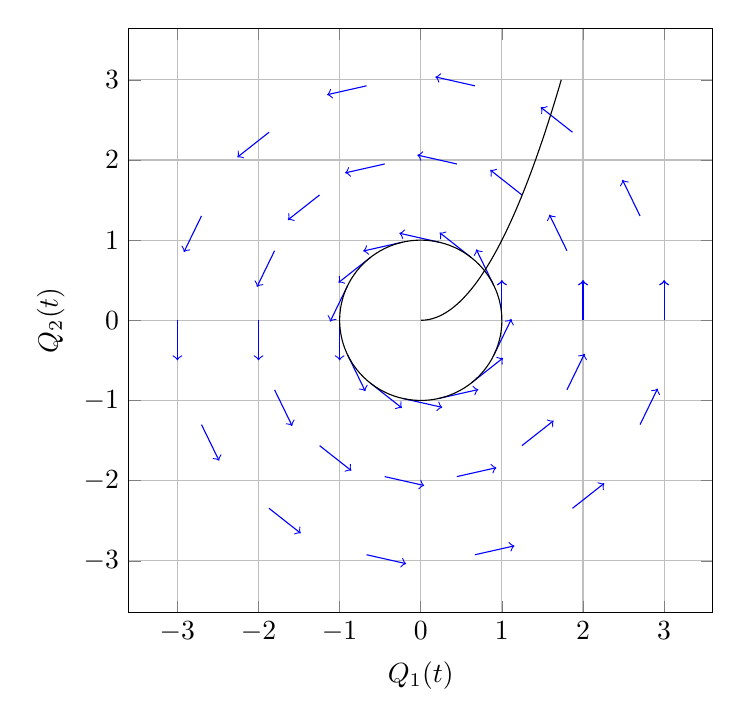
\begin{tikzpicture} 
\begin{axis}[grid=major,xlabel=$Q_1(t)$,
  ylabel=$Q_2(t)$] 
\addplot[samples=15, domain=0:2*pi, variable=\t,
quiver={u={-sin(deg(t))}, v={cos(deg(t))}, scale arrows=0.5}, 
  ->,blue]({cos(deg(t))}, {sin(deg(t))});  
\addplot[samples=15, domain=0:2*pi, variable=\t,
quiver={u={-sin(deg(t))}, v={cos(deg(t))}, scale arrows=0.5}, 
  ->,blue]({2*cos(deg(t))}, {2*sin(deg(t))});  
\addplot[samples=15, domain=0:2*pi, variable=\t,
quiver={u={-sin(deg(t))}, v={cos(deg(t))}, scale arrows=0.5}, 
  ->,blue]({3*cos(deg(t))}, {3*sin(deg(t))});  
\addplot[samples=100, domain=0:2*pi] ({cos(deg(x))},{sin(deg(x))}); 
\addplot[samples=100, domain=0:sqrt(3)] ({x},{x^2}); 
\end{axis}
\end{tikzpicture}  
% \end{center}
\end{figure}
Now, it is easy to check the corresponding invariance condition first
introduced in (\ref{SimpleCDC}). Let $G_z(z)$ denote the Frechet
derivative (which in turns is the Jacobian in this deterministic and
finite-dimensional case) of $G$ at $z$. The columns of the matrix
representation of $G_z$ are the tangent vectors above
(\ref{SimpleCDC}), so the tangent space $T_q(\mathcal{S}^1)$ to
$\mathcal{S}^1$ at $q=G(z)$ coincides with the image $Im[G_z(z)]$:
$$
G_z(z)=[ -\sin(z) \;\cos(z) ]^T.
$$
Recall that the vector field $\mu$ at $q=G(z)$ is in turns:
$$
\mu(G(z))=[ -\sin(z) \;\cos(z) ]^T.
$$
We thus trivially have
$$
\mu(G(z)) \in Im[ G_z(z)],
$$
and, in fact, this is the consistency condition we have to check out
for pairs ($\mathcal{M}$,$\mathcal{G}$) when $\mathcal{M}$ is an
autonomous and deterministic differential system of finite dimension.
\newpage\mbox{}\thispagestyle{empty}

 % Geometric Theory
\chapter{The Hull-White Model and multiobjective calibration}  
This chapter is the first chapter with empirical and numerical
applications\footnote{Some of the results presented in this chapter are also
  reported in \cite{FNN:2009}.} of this work. We have shown the
foundations of interest rate theory and we have derived the general
conditions of consistency. However, only little attention has been
devoted to the empirical applications of these concepts. In this
chapter we address these applications. 
\section{The Hull-White Model}
% % % Consider a complete probability space $(\Omega,\mathcal{F},P)$. Let $W$ be a
% % % one dimensional Wiener-Einstein stochastic process defined in this
% % % space. Assume the existence of an integrable
% % Let $W$ be a one dimensional Wiener stochastic process defined in  a
% % complete probability space $(\Omega,\mathcal{F},P)$. 

% Single factor Heath-Jarrow-Morton \cite{HJM:1992} framework is based on the
% dynamics of the entire forward rate curve, $\{r_t(x),~x>0\}$. Thus,
% under Musiel a's \cite{Mu:1993}
% parameterization  it follows that the infinite dimensional diffusion
% process given by
% \begin{equation}
% \label{eq:HJMM1}
% \left\{
% \begin{array}{rcl}
% dr_t(x)& = & \beta(r_t,x) dt + \sigma(r_t,x)dW_t \\
% r_0(x) & = & r^*(x),
% \end{array}
% \right.
% \end{equation}
% where $\{ r^*(x),~x\geq 0\},$ can be interpreted as the {\sl observed} forward rate
% curve.
% % % % Hasta Aqu Revisado
% The standard drift condition derived in Heath, Jarrow and Morton \cite{HJM:1992}
% can easily transferred to the Musiela parametrization (see, for instance,
% Musiela \cite{Mu:1993}),
% $$
% \beta(r_t,x)=\frac{\partial}{\partial x} r_t(x)+\sigma(r_t,x)\int_0^x
% \sigma(r_t,s) ds.
% $$
% Thus, a particular model is constructed by the choice of an explicit volatility
% function $\sigma(r_t,x)$. 

% Recall that our work is devoted tot

Our test case is the following model, studied by Hull and White
\cite{HW:1990} (henceforth HW):
\begin{equation}
\label{HW}
dr(t)=\left[ \Phi(t)-a r(t)\right] dt + \sigma dW(t).
\end{equation} The Hull-White model improve Ho-Lee model incorporating
mean-reversion and providing closed formulas for liquid options like
interes rate caps. This model is one of the simplest Gaussian HJM
models which preserves the Markov property, allowing very efficient
numerical methods for the pricing of any kind of options. On the
negative side, it does not capture large humps of the term structure
of volatilities (TSV hereafter). The model instantaneous-forward
volatility curve $T \to \sigma_f(t,T)$, as we will prove later, is
monotonically decreasing and this fact often allows only small humps
in the caplet curve. However, as pointed out by Brigo and Mercurio
\cite[pp. 91--92]{BM:2006}, in case of decreasing TSIR curves, large 
humps can be produce even by this model. 

Summarizing, it exhibits a relative good performance when it is chosen
as a parsimonious solution for bussiness cycles with monotonically
decreasing TSV, as it is shown by \cite{AH:2005}.   % The classical HJM forward rate formulation for the HW model is
% \begin{equation}
% \label{HWHJM}
% dF(t,T)=\alpha(t,T)\: dt+\: \sigma(t,T) dW(t),
% \end{equation}
% with $\sigma(t,T)=\sigma e^{-a(T-t)}$. We will establish with
% precision the equivalence between this forward formulation and the
% original one (\ref{HW}) in the following lines. 
\subsection{Markovianity of the HW model}
The short-rate differential process (\ref{SRMHJM}) in Proposition 2 is
not a Markov process in general. Notice in fact that time $t$ appears in the
expression (\ref{driftSRMHJM}) for the drift both as extreme of
integration and inside the integrand function. However, the HW model
as a particular Gaussian HJM have a suitable specification of $\sigma$
for which the short-rate $r$ is indeed a Markov process. This happens
because we can write the model volatility function $\sigma(t,T)$ as a
separable specification:
\begin{equation} 
\label{diffusionHWHJMseparable}
\sigma(t,T)=\varsigma(t)\varrho(T)
\end{equation} 
with $\varsigma(t)$ and $\varrho(T)$ strictly positive and deterministic
functions of time. Under such a separable specification, the
short-rate process becomes
\begin{equation}
\label{intSRM}
\begin{array}{rcl}
r(t):=F(t,t)&=&F(0,t)+\int_0^t \left(\varsigma(u)\varrho(t)\int_u^t
  \varsigma(u) \varrho(s)\: ds\right)\: du +\int_0^t \varsigma(s)
\varrho(t)\: dW(s) \\ 
&=& F(0,t)+\varrho(t)\int_0^t \left(\varsigma^2(u)\int_u^t \varrho(s)
  \:ds \right)\:du +\varrho(t) \int_0^t \varsigma(s) \: dW(s) 
\end{array}
\end{equation}
Notice that, if we introduce the deterministic function $A(\cdot)$  
$$
A(t):=F(0,t)+\varrho(t) \int_0^t \left( \varsigma^2(u) \int_u^t \varrho(s)
ds\: \right) du,
$$
by taken differentials in (\ref{intSRM}) we can write
\begin{equation}
\label{diffSRM}
\begin{array}{rcl}
dr(t)&=& A'(t)+\varrho'(t) \int_0^t \varsigma(s) dW(s)
+\varsigma(t)\varrho(t)\: dW(t)\\ 
&=& \left[ A'(t)+\varrho'(t) \displaystyle\frac{r(t)-A(t)}{\varrho(t)}\right]\:
dt+\varsigma(t)\varrho(t)\: dW(t)\\
&=& \left[ a(t)+b(t) r(t)\right]\:dt+c(t)\: dW(t)
\end{array}
\end{equation}
where \begin{equation}
\begin{array}{rcl}
a(t) &:=& A'(t)-\displaystyle\frac{\varrho'(t)}{\varrho(t)}A(t),\\ 
b(t) &:=& \displaystyle\frac{\varrho'(t)}{\varrho(t)}\; \textrm{; and,}\\
c(t) &:=& \varsigma(t)\varrho(t)=\sigma(t,t).
\end{array}
\end{equation}
We can finally derive the HJM forward-rate dynamics that is equivalent
to the original short-rate dynamics (\ref{HW}). To this end, let us
set
$$
\sigma(t,T)=\sigma e^{-a (T-t)},
$$
where $a$ and $\sigma$ are real constants, so that
\begin{equation}
\label{defHWHJM}
\begin{array}{rcl}
\varsigma(t)&=&\sigma e^{a t},\\
\varrho(T)&=&e^{-a T},\\
A(t)&=&F(0,t)+\frac{\sigma^2}{2 a^2}(1-e^{-a t})^2;
\end{array}
\end{equation}
and after some tedious but trivial algebra we have for the HW model:
 \begin{equation}
\begin{array}{rcl}
  a(t) &:=& F_t(0,t) +a F(0,t)+\displaystyle\frac{\sigma^2}{2a}(1-e^{-2 a t}),\\ 
b(t) &:=& -a\\
c(t) &:=& \sigma.
\end{array}
\end{equation}
The resulting short-rate dynamics is then given by
\begin{equation}
\label{HWfinal}
dr(t)=\left[F_t(0,t)+aF(0,t)+\displaystyle\frac{\sigma^2}{2a}(1-e^{-2
    a t}) -a r(t)\right]\: dt+\sigma\: dW(t),
\end{equation}
which is equivalent to (\ref{HW}) when combined with the identity
$$
\Phi(t):=F_t(0,t)+a F(0,t)+\displaystyle\frac{\sigma^2}{2a}(1-e^{-2 a t}).
$$
In conclusion, we then have that the HW model is a short-rate
markovian model that admits a one-factor HJM formulation. Turning back
to the Musiela parametrization, we have that the volatility
specification for this model is \begin{equation}
\label{volHWHJMM}
\widetilde\sigma(t,x):=\sigma(t,t+x)=\sigma e^{-a x},
\end{equation}
which falls into the class of HJM models with deterministic
volatility $$\widetilde\sigma(f_t,x)=\widetilde\sigma(x).$$ 
\section{The Nelson and Siegel family and Invariance}
In order to illustrate the theoretical ideas shown in the previous
chapter, we now move from abstract theory to the investigation of a
number of concrete forward curve families and the Hull-White
model. More fundamental results can be found in Bj\"ork and
Christensen \cite{BC:1999} in detail. The leading example is the
popular forward curve family introduced by Nelson and Siegel
\cite{NS:1987}, first introduced informally in previous chapter. We
analyze the consistency of this family and several variations of it
with the Hull-White model. We adapt some of the theoretical results to
this Gaussian case study without no further technical discussion for
the general case. From now, we again remove the symbol
$\;\widetilde{}\;$ as in Chap. 4., i.e. we will consider the HJM model 
under the Musiela parametrization. 

Consider the space $\mathcal{H}_\gamma$ introduced in
Sect. 4.3.2 \begin{corol} Consider as given the mapping 
$$
G: \mathcal{Z} \to \mathcal{H}_\gamma
$$
where the parameter space $\mathcal{Z}$ is an open connected subset of
$R^d$, $\mathcal{H}_\gamma$ a Hilbert space and the {\sl forward curve
  manifold} $\mathcal{G}\subseteq H_\gamma$ is defined as
$\mathcal{G}={\rm Im}(G)$.  The family $\mathcal{G}$ is consistent with the 
one-factor model $\mathcal{M}$ with deterministic volatility function
$\sigma(\cdot)$, if and only if
\begin{eqnarray}
\label{gCDC}
G_x(z,x)+\sigma(x)\int_0^x \sigma(s) ds & \in & Im\left[G_z(z,x)\right],\\    
\label{gCVC}
\sigma(x) & \in & Im\left[G_z(z,x)\right],	
\end{eqnarray}
for all $z\in Z$.
\end{corol}
\begin{demo}
See Theorem 4 in Sect. 4.3.2 for the particular case of deterministic
volatility $\sigma(f_t,x)=\sigma(x)$. 
\end{demo}

The statements (\ref{gCDC}) and (\ref{gCVC}) are the particular CDC
and CVC for the deterministic volatility case. These are easy to apply
in concrete cases as shown Bj\"ork and Christensen \cite{BC:1999} or
De Rossi \cite{R:2004}, among others.  
\subsection{The NS family}
The NS forward curve manifold $\mathcal{G}$ is parametrized by $z\in
\mathcal{Z}=\mathbb{R}^4$. Recall that the curve shape $G(z, x)$ is
given by the expression
\begin{equation}
\label{NSspec}
G(z,x)=z_1+z_2 e^{z_4 x}+z_3 x e^{-z_4 x}.
\end{equation}
For $z_4=0$ the {\sl Frechet} derivatives $G_z(z,x)$ and $G_x(z,x)$
are easily obtained as
\begin{equation}
\label{rcl}
\begin{array}{rcl}
G_z(z,x) &=& [1\quad e^{-z_4 x}\quad xe^{-z_4 x}]^T,\\
G_x(z,x) &=& (z_3-z_2 z_4 -z_3 z_4 x)e^{-z_4 x}.
\end{array}
\end{equation}
Henceforth, we write $\mathcal{Z}_{NS}=\{ [z_1\; z_2\; z_3\; z_4]^T\;
: z_4\neq 0\}$ for the NS parameter space and
$\mathcal{G}_{NS}=G(\mathcal{Z}_{NS})$ for the associated
manifold. For the HW model characterized by the volatility function
(\ref{volHWHJMM}), the consistency conditions of Theorem 4 become
\begin{equation}
\left\{
\begin{array}{rcl}
G_x(z,x)+\frac{\sigma^2}{a}\left[ e^{-a x}-e^{-2 a x}\right] & \in &
Im[ G_z(z,x) ], \\
\sigma e^{-a x} & \in & Im[ G_z(z,x) ].
\end{array}
\right.
\end{equation}
To investigate whether $\mathcal{G}_{NS}$ is invariant under HW
dynamics, we consider now simplest consistency condition, the CVC: let
us consider for constants $\alpha_i$, such $\forall x\geq 0$ we have  
\begin{equation}
\label{NSCVC}
\sigma e^{-a x}=\alpha_1 + \alpha_2 e^{-z_4 x}+\alpha_3 x e^{-z_4
  x}-\alpha_4 (z_2+ z_3 x) x e^{-z_4 x}.
\end{equation}
One can easily see that is is possible iff $z_4=a$. So as a first
hint, let us fix $z_4=a$ in the parametrization and introduce the
restricted NS family: 
$$
G(z,x)= z_1+z_2 e^{-a x} + z_3 x e^{-a x}.
$$
Now the CVC is verified, while in the CDC we look for $\beta_i$ such
that $\forall x\geq 0$ we have:
\begin{equation}
\label{restricNSCDC}
(z_3-a z_2 -a z_3 x) e^{- a x}+\frac{\sigma^2}{a}\left(e^{-a x}-e^{-2
    a x}\right)=\beta_1+\beta_2 e^{-a x}+ \beta_3 x e^{-a x}.
\end{equation}
This equation can never be verified, due to the extra exponential
$e^{-2 a x}$, so we have proved the following.  
\begin{propos}[Nelson-Siegel and Hull-White.] The Hull-White model is
  inconsistent with the Nelson-Siegel family.
\end{propos}
Let us include this extra exponential in the parametrization, thus, we
finally introduce the augmented NS family:  
$$
G_{ANS}(z,x)=z_1 + z_2 e^{-a x} + z_3 x e^{-a x}+ z_4 e^{-2 a x}.
$$
Now, both CDC and CVC are verified for this family. 
\begin{propos}[Augmented Nelson-Siegel and Hull-White.] The augmented
  Nelson-Siegel family is consistent with the Hull-White model.
\end{propos} 
\begin{demo}
The Frechet derivatives are in this case 
\begin{equation}
\label{rcl}
\begin{array}{rcl}
\displaystyle\frac{\partial G_{ANS}}{\partial z} (z,x) &=& [1\quad e^{-a x}\quad xe^{-a
  x}\quad e^{-2 a x}]^T,\\[.2cm]
\displaystyle\frac{\partial G_{ANS}}{\partial x} (z,x) &=& \left[ z_3-a\left( z_2 + z_3
    x\right)\right] e^{-a x}-2 a z_4 e^{-2 a x}.  
\end{array}
\end{equation}
Now the set $Im[ \partial_zG_{ANS}]$ is ``large'' enough to trivially
satisfy CVC and CDC due to the extra component $e^{-2 a x}$. The
derivation of the balancing equations analogous to (\ref{NSCVC}) and 
(\ref{restricNSCDC}) are left to the meticulous reader. 
\end{demo}

\section{The Minimal Consistent family and Realizations of Gaussian Models} 
It should be also noted that $\sigma(x)$ is a one dimension {\sl
  quasi-exponential} function (QE for short), because is of the form 
\begin{equation}
\label{QE}
f(x)=\sum_i e^{\lambda_i x}+\sum_i e^{\alpha_i x}[p_i(x)\cos(\omega_i
x)+q_i(x)\sin(\omega_i x)],
\end{equation}
with $\lambda_i,\alpha_i,\omega_i$ being real numbers and $p_i, q_i$ are real
polynomials.  

If $f(x)$ is a $q$-dimensional QE function, then it admits the
following matrix representation  
\begin{equation}
\label{VolMatrixForm}
f(x)=c e^{A x} B,
\end{equation}
where $A$ is a $(n \times n)$-matrix, $B$ is a $(n\times q)$-matrix
and $c$ is a $n$--dimensional row vector, see Bj\"ork \cite[Lemma 2.1,
p. 13]{B:2003}. 
Thus, $\sigma(x)$ can be written as 
\begin{eqnarray}
\label{eq:TSVMatrix}
\sigma(x)& = & ce^{A x} b, \text{ where } \\
\nonumber 
c& =& 1,\\
\nonumber
 A& =& -a,\\
\nonumber
 b & = & \sigma.
\end{eqnarray}
We can write the forward rate equation (\ref{HJMM:3}) following
Bj\"ork \cite[Proposition 2.1, pp. 8--9]{B:2003}  
\begin{eqnarray}
\label{eq:Input}
dq_t(x) & = & \mathbf{F}q_t(x)\:dt+\sigma(x)\:dW_t,\quad q_0(x)=0\\
\label{eq:ForwardDecomposition}
f_t(x) & = & q_t(x)+\delta_t(x),
\end{eqnarray}
here $\mathbf{F}$ is a linear operator that is defined by 
$$
\mathbf{F}=\frac{\partial}{\partial x},
$$
and $\delta_t(x)$ is the deterministic process given by
$$
\delta_t(x)=f^o(x+t)+\int_0^t \Sigma(x+t-s)\: ds,
$$
with $$
\Sigma(x)=\sigma(x)\int_0^x \sigma(s)\: ds.
$$ 
Moreover, $q_t(x)$ has the concrete {\sl finite dimensional} realization 
\begin{eqnarray}
\label{eq:Factor}
dZ_t & = & -a Z_t\:dt+\sigma\:dW_t,\quad Z_0=0,\\
q_t(x) & = & e^{-a x}Z_t,
\end{eqnarray}
as a particular result from \cite[Definition 2.1, p. 7]{B:2001} with
the fundamental concluding remark derived by Bj\"ork for QE
deterministic volatilities in \cite[Proposition 2.3,
p. 13]{B:2001}. The SDE (\ref{eq:Factor}) is linear in the narrow
sense \cite{KP:1999}, with explicit solution
\begin{equation}
Z_t=\sigma e^{-a t}\int^t_0 e^{a s}\:dW_s,
\end{equation}
Now, with the definition of $S(x)=\int^x_0 \sigma(u) du$, it is easy to obtain that
$$
\int^t_0 \Sigma(t+x-s)\: ds=\frac{1}{2}\left[S^2(t+x)-S^2(x)\right],
$$
and, therefore, combining these explicit results with decomposition
(\ref{eq:ForwardDecomposition}) we arrive to the forward rate dynamics
\begin{equation}
\label{eq:MC}
f_t(x)=f^o(x+t)+\frac{1}{2}\left[S^2(t+x)-S^2(x)\right]+e^{-a x}Z_t.
\end{equation}
Equation \eqref{eq:MC} may be used for building initial forward rate
curves $f^o(x)$ time-consistent with the model.  

% %{\Large \bf Appendix}
% %\appendix
% \subsection{Consistent Curves with the Model}
% If we want to measure the actual impact that alternative choices to the
% Nelson-Siegel yield curve interpolating approach produces on derivatives pricing and hedging, we need 
% to determine consistent families for this particular model. 
% We adapt some of them to our Gaussian case study without further technical discussion for the general case.
% \begin{defn} Consider the space $\mathcal{H}$ is defined as the space
%   of all $\mathcal{C}^\infty$-functions, 
% $$
% r: \mathcal{R}_+ \to \mathcal{R}
% $$
% satisfying the norm condition:
% $$
% ||r||^2=\sum_{n=0}^\infty 2^{-n} \int_0^\infty \left(\frac{d^n r}{dx^n}(x)\right)^2 e^{-\gamma x}\: dx<\infty
% $$
% where $\gamma$ is a fixed positive real number. 
% \end{defn}
% \begin{tma}[Bj\"ork and Christensen] Consider as given the mapping
% For the particular one-factor model we consider along this work,
% Proposition 7.2 and 7.3 in Bj\"ork and Christensen \cite{BC:1999} may
% be directly applied to get the useful result: 

\subsection{The Minimal Consistent family}
\begin{propos} The family
\begin{equation}
\label{MCF}
G_{MIN}(z,x)=z_1 e^{-a x}+z_2 e^{-2 a x},
\end{equation}
is the minimal dimension consistent family with the model
characterized by $$\sigma(x)=\sigma e^{-a x}.$$
\end{propos}

%Moreover, it should be also noted that {\sl augmented} families related from the
%(\ref{MCF}) can be constructed by adding to $G_m$ an arbitrary function $\phi,$ that is,
%the map
%$$
%G(z,x)=G_m(z,x)+\phi(z,x),
%$$
%is also consistent with this model.
\begin{demo}
As we mentionead earlier, there is a way to justify (\ref{MCF})
focusing on forward rate evolution deduced at (\ref{eq:MC}) we
describe it next. By the definition of $S(x)$, we have that
$S'(x)=\sigma(x).$ Then it is easy to derive that deterministic term  
$\frac{1}{2}\left[S^2(t+x)-S^2(x)\right]$ is of the form
$$
g(t)e^{-a x}+h(t) e^{-2 a x}.
$$ 
Thus, the forward rate evolution becomes
\begin{equation}
\label{eq:MCexp}
f_t(x) =f^o(x+t)+\left( g(t)+Z_t \right) e^{-a x}+h(t)e^{-2 a x}.
\end{equation}
From (\ref{eq:MCexp}) we see that a family which is invariant under time translation is
consistent with the model if and only if it contains the linear space
$\{e^{-ax},e^{-2ax}\}$. 
\end{demo} 

It should be also noted that the map 
$$
G(z,x)=G_{MIN}(z,x)+\phi(z,x),
$$
where $\phi(\cdot)$, is an arbitrary function, is also consistent with this model.

%Moreover, it should be also noted that {\sl augmented} families related from the
%(\ref{MCF}) can be constructed by adding to $G_m$ an arbitrary function $\phi,$ that is,
%the map
%$$
%G(z,x)=G_m(z,x)+\phi(z,x),
%$$
%is also consistent with this model.
%Consequently, to make a
%consistent version of a translation invariant family $\phi(z,x)$ it is enough to
%add $G_m(z,x)$.
Finally, we list some concluding remarks about the families analyzed.
\begin{lema}
The following hold for the Hull-White model 
\begin{itemize}
\item The Nelson-Siegel family (henceforth NS)
$$
G_{NS}(z,x)=z_1+z_2e^{-z_4 x}+z_3 x e^{-z_4 x},
$$
is not consistent with the model. % {\sl CVC} constraint requires $z_4=a$, and
% then, the restricted NS family violates {\sl CDC} condition.
\item The family 
$$
G_{MIN}(z,x)=z_1 e^{-a x}+z_2 e^{-2 a x},
$$
is the lowest dimension family consistent with the model (hereafter MIN).
\item The family
$$
G_{ANS}(z,x)=z_1+z_2e^{-a x}+z_3 x e^{-a x}+z_4 e^{-2 a x},
$$
is the simplest adjustment based on restricted NS family that allows model
consistency (hereafter ANS).
\end{itemize}
\end{lema}
% \subsection{Interest Rate Option Pricing} 

\section{Calibration to Market Data Approaches}
To calibrate the model by means of real data, we actually need to
determine the vector of parameters $\boldsymbol
p=[\:\sigma\:a\:]^T$. In order to estimate the forward rate
volatility,  the statistical analysis of past data can be a possible
approach, but the practitioners usually prefer implied volatility,
laying within some derivative market prices, based techniques. This
way involves a minimization problem where  the loss function can be
taken as  
$$
l_C(\boldsymbol p)=\sum^n_{i=1}(C^o_i- C_i(\boldsymbol p))^2,
$$
where $ C_i(\boldsymbol p)$ are the $i$--th theoretical derivative price and
$C^o_i$ is the $i$--th market price one. As we proved on Sect. 3.2,
the model price, at $t=0$, of the cap with equidistant 
settlement periods is given by 
\begin{equation}
\label{eq:expTheoCap}
C=\sum_{j=1}^n \gamma_j = (1+\tau K) \left(\sum_{j=1}^n \kappa
  P_{j-1}(0)N(-d_-)-P_j(0)N(-d_+)\right),
\end{equation} 
where the $d_{\pm}$ are given by (\ref{capletd+-}). 
Moreover, recall that $P_j(0)$ is the initial $x_j$-maturity discount
bond price $P(0,x_j)$, $\kappa$ equals to $(1+\tau K)^{-1}$ with $K$
denoting the {\sl cap rate}. The volatility function
$\vartheta(0,\cdot)$ defined by the expressions (\ref{volmain}) to
(\ref{volaux}) take the particular form for the HW model:
$$ 
\vartheta(0,x_j)=\frac{\sigma}{a}\left( 1-e^{-a \tau} \right)
\sqrt{\frac{1-e^{-2 a x_j}}{2 a}}. 
% Se puede meter demo en Appendix C (optional) %,$ here $N=7.$ 
$$
The equations (\ref{capletd+-}) and (\ref{eq:expTheoCap}), also
express the effective influence of {\sl ab initio} discount bond curve
estimation on cap pricing.%\footnote{See Appendix}  

The calibration procedures can be described formally as follows. 

Let $\boldsymbol p$ be the parameter vector 
$$[\sigma\:a]^T$$ 
for the model under consideration. Assume that we have time series
observations of the flat volatilities $\bar\sigma_i$ of $N$
at-the-money caps $C_i$ which mature at $T_i$-times where
$i=1,\dots,N$. Suppose we are also equipped with the discount bond
curve estimation, $P(0,x)$, at time $t=0$. As we introduce in
Sect. 3.1, market participants translate volatility quotes to cash
quotes adopting Black model \cite{B:1976}. Thus, according to the
Definition 15 in Sect. 3.1., the market price, at $t=0$, of the cap
with regular payment periods is given by
\begin{equation}
\label{eq:expMktCap}
C^o=\sum_{j=1}^n \gamma^o_j = \tau \sum_{j=1}^n P_j(0)\left(L_j(0)
  N(d_1)-K N(d_2)\right),
\end{equation}  where $d_1$ and $d_2$ are given by the identities
(\ref{d1}) to (\ref{d2}). 

In addition, recall that according to Remark 2 in Sect. 3.1.1 the cap  
 rates for the ATM plain vanilla caps must fulfill
 (\ref{ATMStrikeCap}). % they make the well-known convention that
                       % $K_i$ quantities must be equal to  
% \begin{equation}
% \label{eq:Kswap}
% K_i=\frac{D(\tau)-D(T_i)}{\tau \sum_{j=1}^n D(x_j)},
% \end{equation}
% where $\tau=x_{j+1}-x_j$ is the length of the underlying caplets. 
% The derivation of the formula (\ref{eq:Kswap}) can be found, 
% for example, in Bj\"ork \cite{B:2004} (Proposition 20.7 on pages
% 312--313).
By direct inspection, it is clear that this market convention makes
the rates $K$ depend on the discount bond curve estimation
$P(0,x)$. Let us denote the market prices of caps by 
$$C^o\left(T_i,P(0,x),K_i(P(0,x)),\bar\sigma_i\right).$$ Notice that this expression
emphasizes explicit and implicit dependence  (through ATM {\sl
  strikes}) on discount bond curve estimation even for market
prices. Let $$C\left(T_i,P(0,x),K_i(P(0,x)),\boldsymbol p\right),$$ be the
corresponding theoretical price under our particular model.

\subsection{The Two-Step Traditional Method}
Suppose that we are standing at time $t=0$, the fixed time of
calibration under study. For simplicity from now, we remove the
dependency on initial time $t=0$ from discount bond curve
$P(0,x)\equiv P(x)$. First, we choose a non-consistent parametrized
family of forward rate curves $G(z,x)$. 

Let $P(z,x)$ be the zero-coupon bond prices produced by $G(z,x)$. 
$$
P(z)= \left[\:P_1(z)\:\dots\:P_M(z)\:\right]
$$
Let $P^o_k$ be the corresponding discount $x_k$-bond observations with
$x_k$-times running from $k=1,\dots,M$
$$
P^o= \left[\:P^o_1\:\dots\:P^o_M\:\right].
$$
For each zero-coupon bond denoted with subscript $k$,
the logarithmic pricing error\footnote{Recall that, for small
  $\epsilon_k$, it is also the relative pricing error
  $\frac{P^o_k-P_k(z)}{P^o_k}$.} is written as follows  
$$
\epsilon_k(z)=\log P_k^o-\log P_k(z).
$$
Then, we have chosen in this work the sum of squared logarithmic pricing errors,
$l_P$, as the objective loss function to minimize:
\begin{equation}
\label{eq:minD}
\underset{z}{\textrm{min}}\:l_P(z)=\underset{z}{\textrm{min}}~\|\log
P^o-\log
P(z)\|^2_2=\underset{z}{\textrm{min}}\sum_{k=1}^M\epsilon^2_k(z),  
\end{equation}
with 
$$\log P_k(z)=-\int_0^{x_k} G(z,u)\: du.$$
Now, via the least squares estimators $\hat{z},$ an entire discount
bond curve estimation allows the pricing of caps using the market
practice or the HW model. Following a similar scheme for the
derivatives fitting as in the preceeding lines, we have  
$$
\eta_i(\boldsymbol p)=\log  C_i^o-\log  C_i(\boldsymbol p),
$$ and
\begin{equation}
\label{eq:minC}
\underset{\boldsymbol p}{\textrm{min}}\:
l_C(\boldsymbol p)=\underset{\boldsymbol p}{\textrm{min}}~\|\log  C^o-\log
C(\boldsymbol p)\|^2_2=\underset{\boldsymbol p}{\textrm{min}}\sum_{i=1}^N\eta^2_i(\boldsymbol p),  
\end{equation}
with the vector definitions:
\begin{eqnarray}
C^o&=& \left[\:C^o_1\:\dots\:C^o_N\:\right]\\
C(\boldsymbol p) &=& \left[\:C_1(\boldsymbol p)\:\dots\:C_N(\boldsymbol p)\:\right].
\end{eqnarray}
Note that here we have dropped the dependencies
$(P(x),\:K,\:T,\:\bar\sigma$)  for simplicity. Moreover, notice that
the discount bond curve estimation is external to the model in the
sense that there is no need to know first any of the model parameters
$\boldsymbol p$ for solving non-linear program (\ref{eq:minD}).

\subsection{The Joint Calibration to Cap and Bond Prices}

    Let us now describe in detail the joint cap-bond calibration procedure which
    has sense in a consistent family framework. We note that in this situation the
    parameters of the model are determined together with the initial forward
    rate curve. % Recall the simplified derivation for the consistent families used at Section 2.2. 

This is different from the traditional fitting of the Hull-White model, where the two steps are separate, as we discussed before. From the expression (\ref{MCF}), % in the Appendix, we notice the dependency of the family  
we notice the dependency of the family  from the parameter $a$. Let
$G(z,x,a)$ be a family consistent with the HW model (for instance,
$G_{MIN}$ and $G_{ANS}$) and define least-squares estimators, $\hat{z}(a)$
\begin{equation}
\label{minDcons}
\hat{z}(a)=\arg \underset{z}{\min} \sum_{k=1}^M(\log P^o_k-\log P_k(z,a))^2. 
\end{equation}
From the expression 
\begin{equation}
\label{eq:defM}
\log  P_k(z,a)=-\int_0^{x_k} G(z,a,u)\:du=\sum_{j=1}^{n_p} M_{kj}(a) z_j,
\end{equation}
we note that, for consistent families and for a fixed $a$ the problem
(\ref{minDcons}) is linear in $z$-parameters (for the $G_{MIN}$ family
$n_p=2$, and for the $G_{ANS}$ family $n_p=4$). Thus, $\hat{z}$ is an
explicit and continuous function of $a$. 

Strictly speaking, joint calibration must be formalized as a
multiobjetive optimization problem (MOO) of the form:   
\begin{equation}
\underset{\boldsymbol p}{\min}\;\boldsymbol{l}(\boldsymbol p)
\end{equation}
where
$\boldsymbol{l}=[l_1(\boldsymbol p)\:l_2(\boldsymbol p)]^T$ is
an objective function vector and $\boldsymbol p$ is the {\sl
  design} vector $[\:\sigma\:a\:]^T$. Notice that in this case there
are two objectives and two design variables. The {\sl partial loss
  functions} $l_i(\sigma,a)$ are defined as 
\begin{equation}
\begin{array}{rcl}
l_1(\boldsymbol p) & = & ~\|\log C^o\left[P(\hat{z}(\boldsymbol
  p),\boldsymbol p)\right]-\log C\left[P(\hat{z}(\boldsymbol
  p),\boldsymbol
  p),\boldsymbol p\right]\|^2_2  \\ \nonumber 
l_2(\boldsymbol p) & = & ~\|\log
P^o-M(\boldsymbol p)\hat{z}(\boldsymbol p)\|^2_2
\end{array}
\end{equation}
where 
\begin{equation}
\hat{z}(\boldsymbol p)=R(a)Q^{-1}(a)\log P^o
\end{equation}
being $Q$, $R$ the matrices of the reduced QR decomposition of $M(\boldsymbol p)$
which is defined by the relation (\ref{eq:defM}).

% $l_1(\boldsymbol p)  =  ~\|\log
% C^*\left(D(z,\boldsymbol p)\right)-\log 
% C\left(D(z,\boldsymbol p),\boldsymbol p\right)\|^2$ and
% $l_2(\boldsymbol p)  =  ~\|\log D^*-\log 
% D(z,\boldsymbol p)\|^2$  % because is very improbable that $l_C$ and $l_D$
% would be {\sl extremized} by the same set of parameters,
% $\boldsymbol p^*$.   

Note that it is highly probable that these objectives would both be
conflicting, in general, and no single $\boldsymbol{\hat p}=(\hat
\sigma,\hat a)$ would generally minimize simultaneously the pair of
objective functions $l_i$. Tipically here, there is no single, global
solution, and often, it is necessary to determine a {\sl set} of
points that all fit a predetermined definition for an optimum. Thus,
the predominant concept in defining is that of Pareto optimality
\cite{P:1906}.  

One of the most common and basic approach for multiobjective
optimization requires to build a weighted sum of the objectives (see
for instance \cite{EKO:1990,M:2005}). The result is the following
scalarized utility function, which is minimized: 
 \begin{equation}
\label{Utility}
\tilde l=\omega_1 l_1+\omega_2 l_2.
\end{equation} 
When an appropriate set of solutions is obtained by the
single-objective optimization of $\tilde l$, the solutions can
approximate a Pareto front. The weighted-sum method parametrically
changes the weights among objective functions $l_1$ and 
$l_2$ to obtain this Pareto front. If the two weights are positive
then minimizing the utility provides a sufficient condition for Pareto
optimality, which means the minimum of (\ref{Utility}) is always
Pareto optimal \cite[Sect. 4.1.1, pp. 41--42]{M:2005}. Thus,
consistent calibration carried out with consistent families involves
the entire Pareto optimal set, in contrast to the unique solution
appearing in the two-step scalar problem.

At this point, note that the program used by Angelini and Herzel
\cite{AH:2002,AH:2005} in their works, uses a different goal
attainment 
\begin{equation}
\label{eq:minConsAH}
\underset{\boldsymbol p}{\min}\: l_1(\boldsymbol p)
\end{equation}
where $l_1(\boldsymbol p)$, and $\hat{z}(\boldsymbol p)$ are
defined trough the identities (\ref{eq:minC}) and (\ref{minDcons}). As
a consequence, the program used by these authors is a degenerate case
of (\ref{Utility}) with $\omega_1$ fixed equal to 1 and
$\omega_2$ to 0, so it just allows to obtain one point of the implied
trade-off front, which would be potentially only a weak Pareto
optimum\footnote{Pareto optimal points are WPO, but WPO are not Pareto
optimal.} (WPO) not a standard Pareto optimum \cite[Sect. 4.1.1,
p. 42]{M:2005}. 

 % With yield-curve estimation implemented for every
% fixed $a$, the entire discount function $D(\hat{z}(\boldsymbol p),x,a)$ may be
% determined and it could be thought that the estimates $\hat{\boldsymbol p}$ have to
% be 
% found by solving the non-linear program
% \begin{equation}
% \label{eq:minCcons1}
% \begin{split}
% SSE_C = & \underset{\boldsymbol p}{\min} ~\|\log
%  C^*\left[D(\hat{z}(\boldsymbol p))\right]-\log 
%  C\left[D(\hat{z}(\boldsymbol p),\boldsymbol p,T)\right]\|^2 =\\
% = & \underset{\boldsymbol p}{\min}\sum_{i=1}^N\varepsilon^2_i(\boldsymbol p).
% \end{split}
% \end{equation}
% However, following the latter program we are not sure that the corresponding
% yield-curve 
% at the minimum $\hat{\boldsymbol p}$, $D(\hat{z}(\hat{\boldsymbol p}),x,\hat{\boldsymbol p})$, was
% the optimal value of the sequence of yield curve estimations implicit in this
% program (\ref{eq:minCcons1}). In other words, there exist reasonable doubts
% abouth the convergence 
% of this algorithm, in the sense of obtained the minimization of the pricing
% errors of the cap and zero-coupon bond at the same time. Now, we consider the
% following 
% decomposition for the total loss function $SSE(\boldsymbol p)$
% \begin{eqnarray}
% SSE_D(\boldsymbol p)&=&\|\log  D^*-M(\boldsymbol p)\hat{z}(\boldsymbol p)\|^2,\\
% SSE_C(\boldsymbol p)&=&\|\log  C^*\left[D(\hat{z}(\boldsymbol p))\right]-\log
% C\left[D(\hat{z}(\boldsymbol p)),\boldsymbol p,T)\right]\|^2. 
% \end{eqnarray}
%   Then, as an heuristic solution, we propose to modify the latter program to
%   include pricing residuals for the discount through the convex combination 
% \begin{equation}
% \label{eq:minCons2}
% SSE_\lambda  = \underset{\boldsymbol p}{\min}\left((1-\lambda)\,
% SSE_D(\boldsymbol p)+\lambda\, SSE_C(\boldsymbol p)\right), 
% \end{equation}
% for some fixed $\lambda\in [0,1]$.
% We test the robustness of this fitting algorithm for the MC family by using
% 1000 
% extractions from three independent uniform distributions as initial guess for
% the parameters, $\boldsymbol p^{(0)}$. As representative input data, $(D^*, C^*)$,
% we use the sample mean along the first 75 trading dates of the second
% (excited) 
% period under study. 
% Figure \ref{CalibTest}, shows the sample mean of the 1000 path iterates
% generated by 
% the algorithm for $SSE_C(\boldsymbol p^{(k)})$ and first contribution,
% $SSE_D(\boldsymbol p^{(k)})$, departing from simulated $\boldsymbol p^{(0)}$. After the
% initial 
% movements on the wrong direction, first contribution corrects its behaviour
% for 
% searching its own minimum. Moreover, the second contribution exhibits a
% correct 
% minimization pattern. Note the slightly better results on both sides with
% smaller 
% $\lambda$. Similar results can be obtained with the ANS family and other
% market scenarios.  

\section{Empirical Results}
%We compare three different estimations of initial yield curve based on
%Nelson-Siegel family (henceforth NS), MC and ANS. 
%
%Our first objective is to test the stability for the implied estimation of the model
%parameters $(\sigma,a)$. We consider mean, standard deviation and
%coefficient of variation of parameter estimates time series. 
In this context the main goal is to analyze the impact that an 
alternative interpolation
scheme has on the fitting capabilities of the model. To this end, we use as a
measure, the daily (on average) relative pricing errors,
hereafter $RPE_C$:
$$
RPE_C=\frac{1}{N} \sum_{i=1}^N \frac{|C^o_i-C_i(\boldsymbol{\hat p})|}{C^o_i}
$$
 The same kind of measure is used for the zero-coupon bond prices and we denote it with
$RPE_B$: 
$$
RPE_B=\frac{1}{M} \sum_{k=1}^M \frac{|P^o_k-P_k(\hat z(\boldsymbol{\hat
    p}),\boldsymbol{\hat p})|}{P^o_k} 
$$
We perform such analysis focusing on US market. The real date consists
of 282 daily observations, between 2/09/2002 and 30/09/2003. The
data set is composed of US discount factors for fourteen maturities
(1, 3, 6, 9 months and from 1 to 10 years) and of implied volatilities
of at-the-money interest rate caps with maturities 1,2,3,4,5,7,10
years. This database is provided by Thomson Reuters Datastream.

% \begin{figure}[p]
% \centering
% \caption{Average of the US market TSIR and TSV with 99\% confidence levels. \label{Market}} 
% \includegraphics[width=\textwidth,height=\textheight]{CapsBondSampleAnalysis.pdf}
% \end{figure}

\begin{figure}[h!]
\centering
\caption{Average of the US market TSIR and TSV with 99\% confidence levels.\label{Market}} 

\begin{minipage}[c]{12cm}
\begin{tikzpicture}
\begin{axis}[width=12cm, xlabel={maturity (yr)}, ylabel={sample mean
    $\bar\sigma$ (\%)}]
\addplot+[error bars/.cd,y dir=both,y explicit] table 
[x=T, y=flatvol, y error=99conflevel] {VolDataStats.dat};
\end{axis}
\end{tikzpicture} 
\end{minipage}

\begin{minipage}[c]{12cm}
\begin{tikzpicture}
\begin{axis}[width=12cm, xlabel={maturity (yr)}, ylabel={sample mean
    TSIR (\%)}]
\addplot+[error bars/.cd,y dir=both,y explicit] table 
[x=x, y=rate, y error=99conflevel] {DataStats.dat};
\end{axis}
\end{tikzpicture}
\end{minipage}

\end{figure}

 As it have been explored before, the daily joint calibration of caps and
 bonds with consistent families must be properly carried out as a MOO
 problem. In doing so, we choose an {\sl a posteriori articulation} of
   preferences, that is, we delay the selection of the solution from
 the palette of solutions after the weighted-method runs. In response
 to this articulation of preferences, the decision-maker imposes
 preferences directly on a set of the potential solution points which
 depicts the Pareto front. In such a context, weights are typically
 chosen such that 
\begin{equation}
\label{ConvexMOO}
\sum_{i=1}^Q \omega_i=1
\end{equation}
with $\boldsymbol\omega\geq \boldsymbol 0$ leading to a convex
combination of objectives and this choice can be more helpful than
unrestricted weights so as not to repeat any weighting vectors in
terms of its relative values 
\cite[Sect. 5.3, pp. 73--74]{M:2005}. According to
this, the weighted-sum method was run for every date in sample with
the fixed weight vector $\boldsymbol{\omega}$ satisfying 
(\ref{ConvexMOO}). In doing so, we assume the same ten uniformly
spread values
\begin{equation}
\label{weightSpectrum}
\omega_1=\frac{1}{10}j  \qquad j=1,2,\dots,10
\end{equation}
and $\omega_2=1-\omega_1$ as the second vector weight component for
all trading dates.

%% Explicacion del Scale Factor (metodo 'scaling')
We use the following transformation scheme of the objectives, which is
often called {\sl scaling} \cite{R:1987}:
\begin{eqnarray}
l_i^\tau&=& \frac{l_i(\boldsymbol p)}{s_i} \\
{\rm with}\qquad\frac{l_1 (\boldsymbol p_0)}{s_1}& \approx & \frac{l_2 (\boldsymbol p_0)}{s_2}
\end{eqnarray}
where $s_i$ are scalar coefficients, and $\boldsymbol p_0$ is a feasible starting
point. This approach ensures the objective functions have similar
orders of magnitude. Thus, the way to solve our joint calibration
problem is to use the weighted-sum method, which is finally stated as:
\begin{equation}
\label{finalMOO}
\underset{\boldsymbol p}{\min}\: \left( \omega_1 \frac{l_1(\boldsymbol
  p)}{s_1}+(1-\omega_1) \frac{l_2(\boldsymbol p)}{s_2} \right)
\end{equation}
with $\omega_1$ discrete values given by (\ref{weightSpectrum}).

Figure \ref{MCParetoFronts} shows the in-sample fitting results
performed by the MIN family for some dates of the sample under
analysis. First of all, notice that efficient frontiers with regular
shapes appear nicely revealing the intrinsic multi-objective nature of
the consistent calibration. Moreover, note that it can be found different 
topologies for this frontiers depending on the date. All the days the
objectives are conflicting, and beyond a certain point of the Pareto
front the better we fit the discount bonds the worse we calibrate the caps
portfolio. However, note that, moving on to the Pareto curve, we can
achieve better results for both components of the vector objective
without a trade-off until the above-mentioned Pareto point is
reached. In other words, the MOO calibration may provide a {\sl
  better} set of results for the calibration of caps that would
produced by single optimizing the scalar objective $l_1(\boldsymbol
p)$. 

\pgfplotstableread{ParetoFronts.dat}{\pareto} 
\begin{figure}[h!]
\centering
\caption{Some daily calibration results for the minimal consistent
  family.\label{MCParetoFronts}}
\begin{tikzpicture}
\begin{axis}[xlabel=$RPE_B (\%)$, ylabel=$RPE_C (\%)$]
\addplot [black, mark=*, mark size=1pt] table [x={x1}, y={y1}] {\pareto};
\addplot [black, mark=*, mark size=1pt] table [x={x2}, y={y2}] {\pareto};
\addplot [black, mark=*, mark size=1pt] table [x={x3}, y={y3}] {\pareto};
\addplot [black, mark=*, mark size=1pt] table [x={x4}, y={y4}] {\pareto};
\addplot [black, mark=*, mark size=1pt] table [x={x5}, y={y5}] {\pareto};
\addplot [black, mark=*, mark size=1pt] table [x={x6}, y={y6}] {\pareto};
\addplot [black, mark=*, mark size=1pt] table [x={x7}, y={y7}] {\pareto}; 
\addplot [black, mark=*, mark size=1pt] table [x={x8}, y={y8}] {\pareto}; 
\addplot [black, mark=*, mark size=1pt] table [x={x9}, y={y9}] {\pareto};
\end{axis}
\end{tikzpicture}
\end{figure} The tables on Figure \ref{ParetoTwoDays} show,
as a numerical example, two different Pareto sets restricting
ourselves to the MIN family, the family with the lowest
dimensionality. If we look on both tables, it must be noted that for a
fixed trading date the best cap fit results may occur with
$\omega_1\neq 1$, even if the objectives are competing.

\begin{figure}[h!]
\caption{Efficient points in the $RPE_B-RPE_C$ space using the method
  of convex combinations for two different days in sample. %  The
  % partial objectives, $\omega_1$ and $\omega_2$ are strong
  % conflicting, for the Day 1 (top). In contrast, the latter ones are
  % more cooperative for the Day 2 
  % (bottom).
  \label{ParetoTwoDays}} 
\begin{center}
{\sc Day 1}\\[.1cm]
\begin{tabular}{cccc}
\hline \hline
$\omega_1$ & $\omega_2$  & $RPE_B$ (\%) & $RPE_C$ (\%) \\
\hline
0.1 &  0.9 &  0.1036 &  11.5795\\
0.2 &  0.8 &  0.1645 &  11.2761\\
0.3 &  0.7 &  0.3160 &  10.2359\\
0.4 &  0.6 &  0.4864 &   8.8214\\
0.5 &  0.5 &  0.6573 &   7.1267\\
0.6 &  0.4 &  0.8136 &   5.3813\\
0.7 &  0.3 &  0.9343 &   4.3329\\
{\bf 0.8} &  {\bf 0.2} &  {\bf 0.9941} & {\bf 3.9132}\\
{\bf 0.9} &  {\bf 0.1} &  {\bf 1.0181} & {\bf 4.0016}\\
{\bf 1.0} &  {\bf 0.0} &  {\bf 1.0287} & {\bf 4.0718}\\
\hline
\end{tabular}
\end{center}

\begin{center}
{\sc Day 2}\\[.1cm]
\begin{tabular}{cccc}
\hline \hline
$\omega_1$ & $\omega_2$  & $RPE_B$ (\%) & $RPE_C$ (\%) \\
\hline
0.1 &  0.9 &0.0902 &6.1874\\
0.2 &  0.8 &0.1574 &5.3478\\
0.3 &  0.7 &0.2295 &4.7551\\
0.4 &  0.6 &0.2944 &4.4395\\
0.5 &  0.5 &0.3499 &4.3203\\
{\bf 0.6} &  {\bf 0.4} & {\bf 0.3962} & {\bf 4.2797}\\
{\bf 0.7} &  {\bf 0.3} & {\bf 0.4345} & {\bf 4.3490}\\
{\bf 0.8} &  {\bf 0.2} & {\bf 0.4670} & {\bf 4.4933}\\
{\bf 0.9} &  {\bf 0.1} & {\bf 0.4930} & {\bf 4.6303}\\
{\bf 1.0} &  {\bf 0.0} &{\bf 0.5138} & {\bf 4.7546}\\
\hline
\end{tabular}
\end{center}
\begin{flushleft} The partial objectives, $\omega_1$ and $\omega_2$ are strong
  conflicting, for the Day 1 (top). In contrast, the latter ones are
  more cooperative for the Day 2 
  (bottom).
\end{flushleft}
\end{figure}

In Figure \ref{tsWeights}, we analize more deeply the latter fact this
time for both, MIN and ANS, consistent families. We plot the daily
distribution of the weight $\omega_1$ which performs the best
calibration for caps in sample data. As for the lowest dimensional
family, most of the days the weight vector
$(\omega_1=0.7,\omega_2=0.3)$ produces the best cap calibration
results and there is a non-negligible number of bussiness dates where
other weights than $\omega_1=1.0$ produce better goals than it. As for
the ANS family, we observe an entirely different distribution, but
once again, we note that the best cap calibration results may be
reached with weights different than $\omega_1=1.0$ and even get a large
number of them with the smallest weight possible, $\omega_1=0.1$. 

\pgfplotstableread{Histograms.dat}{\histo} 
\begin{figure}[h!]
\centering
\caption{Daily empirical distribution of weights with the best $RPE_C$
  for both consistent families as produced by the multi-objective
  calibration. \label{tsWeights}} 
\begin{tikzpicture}
  \begin{axis}[
    ybar,
    ylabel={$\%$},
    height=9cm,
    width=12cm,
    enlarge y limits=false,
    axis lines*=left,
    ymin=0,
    ymax=60,
    legend style={at={(0.5,-0.2)},
      anchor=north,legend columns=-1},
    xtick=data,
    nodes near coords,
    every node near coord/.append style={
      anchor=mid west,
      rotate=70
    }
  ]
    \addplot table [x={w_1}, y={frec}] {\histo};
    \addplot table [x={w_1'}, y={frec'}] {\histo};
    \legend{MIN, ANS}
\end{axis}
\end{tikzpicture}
\end{figure}
For the shake of simplicity, from now on we will only consider the
calibration results obtained with daily weights choices that produce
the best calibration for the caps on every trading date. This {\sl a
posteriori} articulation of preferences may be followed by a
decision-maker which want to use consistent calibration as a good risk
management practice or as an extrapolation tool for marking to market
less liquid interest-rate derivatives. Following this particular
articulation of preferences we choose a single Pareto optimum from
the set that estimates the complete Pareto curve. In Figure
\ref{SumStats}, we compare summary statistics of the parameter
estimates and the in-sample fit measures reported by NS, MIN and ANS
families. In addition, Figure \ref{tsComparison} shows the comparison
of in-sample fitting results in time series. 

\begin{figure}[h!]
\centering
\caption{Time Series Comparison. \label{tsComparison}} 
\begin{tikzpicture}
\begin{axis}[
ylabel={$RPE_C(\%)$},
no markers,
legend style={legend columns=-1},
width=12cm,
height=9cm,
xmin=0,
xmax=280]
\addplot [very thick,black] table [x={t}, y={capMC}] {tseries.dat};
\addplot [black] table [x={t}, y={capANS}] {tseries.dat}; 
\addplot [red] table [x={t}, y={capNS}] {tseries.dat}; 
\legend{MIN, ANS, NS}
\end{axis}
\end{tikzpicture}\vskip 1cm

\begin{tikzpicture}
\begin{axis}[
ylabel={$RPE_B(\%)$},
legend style={anchor=east, legend columns=-1},
no markers,
width=12cm,
height=9cm,
xmin=0,
xmax=280]
\addplot [very thick,black] table [x={t}, y={bondMC}] {tseries.dat};
\addplot [black] table [x={t}, y={bondANS}] {tseries.dat}; 
\addplot [red] table [x={t}, y={bondNS}] {tseries.dat}; 
\legend{MIN, ANS, NS}
\end{axis}
\end{tikzpicture}
\end{figure}

The two consistent families under study report better RPE results when we
restrict the analysis to cap data. For RPE on bonds, only the ANS
family outperforms NS in the sample. Recall that this fact is
acceptable since the MIN family is a forward curve with less number of
parameters than the other ones proposed. Moreover, on caps, note that
the MIN family appears to give better results than its consistent 
counterpart, ANS. Now, this behaviour can be explained because the
major of dates considered, market data make the objective
functions $l_1$ and $l_2$ of this family to strongly conflict as seen
in Figure \ref{tsWeights}.

\begin{figure}[h!]
\caption{Summary statistics for the calibration results. In-sample
  descriptive statistics are carried out using the daily Pareto points
  with the best derivative fit outcomes.\label{SumStats}} 
\begin{center}
{\sc Summary Statistics}\\[.1cm]
\begin{tabular}{cccc}
\hline \hline
 & MIN & ANS & NS \\
\hline
$\sigma$ & 0.0145 & 0.0127 & 0.0164\\
$a$ & -0.0096 & 0.0243 & 0.0256\\
 $C_v(\sigma)$ & 0.1113 & 0.3118 & 0.14\\
$C_v(a)$ & -3.2659 & 2.4268 & 1.8831\\
$RPE_C$ (\%) & 3.3361 & 8.3011 & 8.5458\\
$RPE_B$ (\%) & 0.5688 & 0.061 & 0.0609\\
\hline
\end{tabular}
\end{center}
\end{figure}

\section{Concluding Remarks}
When calibrating the Hull-White model, a TSIR curve choice to fit a
few market data observations is needed. In particular it seems to be
natural to use families of curves which do not modify their structure
under the future evolution of the model, the so-called consistent
families.
 
In this work, we choose three families of curves (two consistent
families and the popular Nelson-Siegel family) and we conclude that
this choice have an effective impact on the quality of in-sample
fitting for US-market data.  Moreover, this paper extends the seminal
calibration algorithm proposed in Angelini and Herzel \cite{AH:2002}.  

In a consistent approach the parameters of the model are
estimated jointly with the esmation of initial discount bond
curve. Therefore, from a rigorous point of view, joint calibration of 
caps and bonds must be viewed as a multi-objective optimization
nonlinear problem. Although the main purpose of the algorithm is to
minimize the relative differences of cap prices too, note that the 
bi-objective extension of the consistent calibration presents more
general features. Such extension is structured to allow more numerical
outcomes and we observe that it allows to better fit results for both,
caps and bonds, than the above mentioned. In particular, it is
possible to find better cap calibration outcomes with $\omega_1\neq
1$, and this is definitively different from what worked Angelini and
Herzel \cite{AH:2002} on Hull-White model, where only the fixed
$\omega_1=1$ seems to be considered for all consistent families. The
empirical findings of this paper show that, in general, consistent
calibration on every date must to be carried out by analyzing the
entire shape of the Pareto curve. 

 In this sense, this work confirms and complements the shown by
 Angelini and Herzel \cite{AH:2002,AH:2005} restricted to a Euro data
 set. We articulate preferences restricting possible outcomes on every
 date, by choosing the Pareto points which are responsible of better
 fit results on caps. Then the minimal consistent family gives the
 best performance in terms of caps pricing errors and becomes a good
 candidate for the calibration of the Hull-White model. The ANS
 consistent family performs very close to the Nelson-Siegel family,
 though it seems to be the best solution for estimating the discount
 bond function. Now, this could be explained in the context of vector
 optimization. We show empirically the usual competing behaviour
 followed by the objectives through the sample considered. Then, the
 minimal parameterized consistent family relax the performance on the
 estimation of the discount bond curve function, allowing minor
 relative pricing errors on caps.   

% \begin{figure}[p]
% \centering
% \caption{Daily calibration results for the minimal consistent family. 
% The sample is divided into two periods for ease of visualization. \label{MCParetoFrontiers} }
% %\includegraphics[width=\textwidth,height=\textheight,clip]{MCParetoFrontiers.eps}
% \includegraphics[width=\textwidth,height=\textheight]{MCParetoFrontiers.pdf}
% \end{figure}



% \begin{figure}[p]
% \centering
% \caption{On top, daily weights of the multiobjective program with the best $RPE_C$ for both consistent families. On the bottom, we choose the daily values which are responsible for the best $RPE_B$. \label{tsWeights}}
% \includegraphics[width=\textwidth,height=\textheight]{BetterWeights.pdf}
% % \includegraphics[scale=0.8,clip]{MCParetoFrontiers.eps}
% \end{figure}




 % Hull-White-
\chapter{Multiojective Calibration: More Empirical Evidence}

In Chapter 5 we have shown that the consistency hypothesis stated by
Bj\"ork \cite{BG:1999,BC:1999}, implies that the discount bond curve 
has to be determined at the same time as the parameters of the
model. Angelini and Herzel \cite{AH:2002, AH:2005}, originally proposed
the use of a optimization program related to the mentioned daily
calibrations, which is compatible with this joint estimation. % Perhaps, 
The milestone of this methodology is the use of an objective function
based on an error measure for just the portfolio of caps. Then, the
theoretical prices for the caps along the minimization of this measure
can be calculated at the same time that the discount bond curve is
fitted. This is an efficient method because consistent families of
discount bond curves have good analytical properties under the
Gaussian hypothesis, i.e. deterministic {\sl forward} volatility.

In last chapter, we have also provided an extension of the above
strategy which involves a multi-objective framework. As a direct
consequence, the objective function above-mentioned, is subtituted by
a {\sl scalarized} form of the intrinsic bi-objective problem. Now,
the error measure for the discount bonds is evaluated in each
iteration and could even dominate the joint optimization problem. To
this scope, we construct this {\sl scalarized} form using a convex
combination of both the cap and the bond error measures, by means of a
set of restricted weights. As a matter of fact, this approach is
richer in possible outcomes. 

%In this paper, we illustrate taking as a case study the daily
%calibrations of european caps, the relevance  in the choice of the
%initial curve. To this scope,  we compare the behaviour of consistent
%and inconsistent families in terms of model parameter stability and
%fitting capabilities. 

%As an obvious consequence, 
%to the cap prices 
% Explicacion Papel I
%In this paper, we illustrate the relevance of the choice of the initial curve in daily
%calibrations by comparing, in terms of model parameter stability and
%fitting ability, the behaviour of consistent and inconsistent
%families. Our analysis incises about the practical implications of
%consistency by means of a consistent family of functions closed to
%the usual non--consistent ones.  

% In doing so, we understand of extraordinary relevance that the joint
% calibration for the caps and bonds that encompasses consistency
% hints as we % will proof later, can be considered as a well-posed
% mathematical problem. As a matter of fact, in this paper, there is a
% clear difference between % %the optimization program which we show,
% a suitable choice for these needs, and the other one that have
% appeared in the financial literature in the % past pursuing similar
% conceptual goals. We remark that Angelini and Herzel
% \cite{AH:2002,AH:2005}, uses an approach for this optimization with
% % a different and less general objective function
% % specifications. Honestly, we do not like this point of view
% % concerning the objective program % % specifications, because in
% % doing it this way, we lose the richness of possible outcomes that
% % our original optimization program reports. This work also %shows
% % how flexible this new approach is in terms of convergence
% % properties.   

% Contestacion-Resumen Papel II

\section{Introduction}
Given the theoretical tools we have developed in the previous
chapters, we want to analyze further empirical results which support
the use of consistent families and the multi-objective calibration
techniques.

To this end, we extend such analysis to a particular humped volatility
HJM model, proposed by Ritchen and Chuang \cite{RC:1999} and Mercurio
and Moraleda \cite{MM:2000}, independently. We have chosen this model 
because it is quite popular and analytically treatable. In particular,
it provides closed formulas for Europeans interest-rate options. Moreover, 
it is a one-factor Gaussian model that seems to be more capable than the
Hull-White model for reproducing large humps in the implied cap
volatility curve. 

We perform our study by calibrating this model, first by using
simulated data and second by focusing on market a data set composed by US discount 
bonds and at-the-money flat cap volatilities quotes in two different
periods, as shown by the Figure \ref{data}.

\begin{figure}[h!]
\begin{center}

\caption{Market TSIR and TSV data in the two different market scenarios.\label{data}}
\begin{minipage}[c]{12cm}
\begin{tikzpicture}
\begin{axis}[width=12cm, xlabel={maturity (yr)}, ylabel={sample mean
    $\bar\sigma$ (\%)}]
\addplot+[error bars/.cd,y dir=both,y explicit] table 
[x=T, y=flatvolS1, y error=2sigmasS1] {VolDataStatsCh6.dat};
\addplot+[error bars/.cd,y dir=both,y explicit] table 
[x=T, y=flatvolS2, y error=2sigmasS2] {VolDataStatsCh6.dat};
\end{axis}
\end{tikzpicture}
\end{minipage}
\begin{minipage}[c]{12cm}
\begin{tikzpicture}
\begin{axis}[width=12cm, 
xlabel={maturity (yr)}, 
ylabel={sample mean TSIR (\%)},
legend style={at={(0.5,-0.2)}, anchor=north,legend columns=-1}
] 
\addplot+[error bars/.cd,y dir=both,y explicit] table 
[x=x, y=rateS1, y error=99conflevelS1] {DataStatsCh6.dat};
\addplot+[error bars/.cd,y dir=both,y explicit] table 
[x=x, y=rateS2, y error=99conflevelS2] {DataStatsCh6.dat};
\legend{Period 1, Period 2}
\end{axis}
\end{tikzpicture}
\end{minipage}

\end{center}
\end{figure}

With regard to the real market data, the first scenario depicts a
market situation where the implied cap volatility curves have a large
long-term humped shape and the term structure of interest rates is
closer to be flat. On the other hand, the second scenario has
periodically resurfaced in the market and may 
be considered more typical. In this situation the peak of the 
hump is at about the two year point. Moreover, the TSIR is not
monotonic increasing nor flat, being initially-inverted with a local
minimum at short-term maturities.

This rest of this chapter is organized as follows\footnote{This
  chapter is based on \cite{FNN:2011,FNN:2008}.}. In Section 6.2 we
give a brief overview of the model we want to consider and later we
discuss how to construct consistent families with such a
model. Section 6.3 is devoted to empirical results, first comparing
the consistent calibration with the non-consistent approach by means
of simulated data, then presenting 
the results of the fitting of the different methods with market data.
In the last section we give some final conclusions and
remarks. \section{Consistent Curves with The Model} Our work is devoted to the
one-dimensional Gaussian HJM humped 
volatility model of the form:
\begin{equation}
\label{HVHJMM}
df_t(x)=\{ \dots \}\,dt+ \left( \alpha + \beta x \right) e^{-a x}\,dW_t.
\end{equation}
Thus, the forward rate volatility function $\sigma(x)$ is
deterministic depending only on time to maturity.
% \begin{equation}
% \label{HVVol}
% \widetilde{\sigma}(x)=(\alpha+\beta x ) e^{-a x}.
% \end{equation}
Note that $\sigma(x)$ is a QE function that admits the matrix
representation (\ref{VolMatrixForm}). Therefore, $\sigma(x)$ may be
rewritten as 
\begin{eqnarray}
\label{eq:HVTSVMatrix}
\sigma(x)& = & ce^{A x} b, \text{ where } \\
\nonumber 
c& =& [\alpha~~\beta-a\alpha],\\
\nonumber
 A& =& \left[\begin{array}{cc}
0  & -a^2 \\
1  & -2a
\end{array}\right],\\
\nonumber
 b & = & \left[\begin{array}{c}
1\\
0
\end{array}\right].
\end{eqnarray}
For this model, the forward rate decomposition
$f_t(x)=\delta_t(x)+q_t(x)$, as seen before in Sect. 5.3,
eqs. (\ref{eq:Input})--(\ref{eq:ForwardDecomposition}), has
the corresponding $q_t$-process dynamics: 
\begin{eqnarray}
\label{eq:HVFactor}
dZ_t & = & A Z_t\:dt+b\:dW_t,\quad Z_0=0,\\
q_t(x) & = & C(x)Z_t,
\end{eqnarray}
with $A,~b$ as in (\ref{eq:HVTSVMatrix}) and $C(x)=c e^{A x}$. % Thus,
% (\ref{eq:Factor}) is a linear SDE in the narrow sense (see 
% Kloeden and Platen \cite{KP:1999} for details) with explicit solution
% \begin{equation}
% Z_t=\Phi_t\int^t_0 \Phi^{-1}_sb\:dW_s,
% \end{equation}
% where 
% $$
% \Phi_t=e^{A t}=e^{-a t}\left[\begin{array}{rr}
% 1+a t & -a^2 t \\
% t & 1-a t
% \end{array}\right].
% $$
Therefore, the analytical expression of the forward rate curve for the model is
given by \begin{equation}
\label{eq:HVHJMMOperational}
f_t(x)=f^o(x+t)+\frac{1}{2}\left[S^2(t+x)-S^2(x)\right]+C(x)Z_t,
\end{equation}
being $S(x)=\int_0^x \sigma(u)\, du$. After some algebraic
manipulations like using the explicit expansion for the stochastic term 
$C(x) Z_t$  
\begin{equation}
\begin{split}
c e^{A x}\left[\begin{array}{c}
Z^1_t\\
Z^2_t
\end{array}\right] & = e^{-a x}\left[\alpha~\beta-a\alpha\right]
\left[\begin{array}{rr}
1+a x & -a^2 x \\
x & 1-a x
\end{array}\right]\left[\begin{array}{c}
Z^1_t\\
Z^2_t
\end{array}\right] \\ \nonumber
& \\
& = e^{-a x} \left(\alpha  Z^1_t-a \alpha 
   Z^2_t+\beta  Z^2_t\right)+x e^{-a x}
   \left(\beta  Z^1_t-a \beta 
   Z^2_t\right),
\end{split}
\end{equation}
and expanding the deterministic term
$\frac{1}{2}\left[S^2(t+x)-S^2(x)\right]$ which is of the form 
$$
g_1(t) e^{-2 a x}+g_2(t)x e^{-2 a x}+g_3(t) x^2 e^{-2 a x}+h_1(t) e^{-a x}+h_2(t) x e^{- 2 a x},
$$  
(\ref{eq:HVHJMMOperational}) may be written as
\begin{equation}
\label{eq:HVMCexp}
\begin{split}
f_t(x) & =f^o(x+t)+ g_1(t) e^{-2 a x}+g_2(t)x e^{-2 a x}+g_3(t) x^2 e^{-2 a x}+  \\ 
&  \left(h_1(t)+\alpha  Z^1_t-a \alpha Z^2_t+\beta Z^2_t\right)e^{-a x}
+ \ \left(h_2(t)+\beta Z^1_t-a \beta Z^2_t\right) x e^{-a x}.
\end{split}
\end{equation}
Note that this formula, as its corresponding counterpart in previous
chapter (\ref{eq:MCexp}), is relevant for consistency, because it
shows which curves the model produces for a given initial curve
$f^o(x)$.
\subsection{The Minimal Consistent family} 

% To calibrate the model by means of real data, we actually need to determine the vector
% parameter $\theta=(\alpha,~\beta,~a)$. In order to estimate the forward rate volatility, 
% the statistical analysis of past data can be a possible approach, but the
% practitioners usually prefer implied volatility, laying within
% some derivative market prices, based techniques. 
% This way involves a minimization problem where 
% the loss function can be taken as
% $$
% l(\theta)=\sum^n_{i=1}(\zeta^*_i-\zeta(\theta,T_i))^2,
% $$
% where $\zeta(\theta,T_i)$ are the $i$--th theoretical derivative price maturing at time $t=T_i$, and
% $\zeta^*_i \equiv \zeta^*(T_i)$ is the $i$--th market price one.  As it is well known, see Proposition 24.15 and pages 364--366 in Bj\"ork \cite{B:2004},  the  price, at $t=0$, of the cap is given by

% % we need to know how this standard derivative contract is made. Suppose the
% %current time is $t=0$. Starting with $t=T$, we proceed backwards in steps of
% %length $\tau$ in time, constructing the the following set of times $x_i=(i+1)\tau$, with $i=0(1)n$ . Then we construct a portfolio of $n$ {\sl caplets}, struck at $K$, with
% %maturities $\{x_0,~x_1,~\dots,x_{n-1}\}$. These are called the fixing
% %dates or caplet maturity dates. The dates $\{x_1,~x_2,~\dots,~x_n\}$ are called the
% %payment dates. The cap is then just equal to this strip of {\sl caplets} and its
% %price is equal to the price of its constituent {\sl caplets}. If $\xi_j$
% %denotes the price at time $t=0$ of a {\sl caplet} with maturity date $x_j$
% %(and payment date $x_{j+1}=x_j+\tau$), then the model price of the cap is
% %given by
% %\begin{equation}
% %\label{eq:theoCap}
% %\zeta(T)=\sum_{j=0}^{n-1}\xi_j.
% %\end{equation}
% %Specifically, the payoff of each individual {\sl caplet} is 
% %$$
% %h_\xi(x_{j+1})=\tau(y_L(x_j,x_j+\tau)-K)^+.
% %$$
% %It is received at time $x_j+\tau$ and $y_L(x_j,x_j+\tau)$ is the spot
% %US--LIBOR rate prevalent over the accrual period $[x_j,x_j+\tau]$ (expressed as a
% %simple compound rate) and with fixing time $x_j$. It follows that, at time
% %$x_j$, the payoff of such a caplet is 
% %$$
% %h_\xi(x_j)=D(x_j,x_j+\tau)\tau(y_L(x_j,x_j+\tau)-K)^+.
% %$$
% %On the other hand, the price of a zero-coupon bond at time $x_j$ and maturing at
% %time 
% %bond may be expressed as 
% %$$
% %D(x_j,x_j+\tau)=(1+\tau y_L(x_j,x_j+\tau))^{-1}.
% %$$
% 	%Thus, it follows that
% %\begin{equation}
% %\begin{split}
% %\nonumber
% %h_\xi(x_j) &
% %=D(x_j,x_j+\tau)\tau\left(\frac{1}{\tau}\left[\frac{1}{D(x_j,x_j+\tau)}-1\right]-K\right)^+\\
% %& \\ 
% % & = \frac{1}{\kappa}(\kappa-D(x_j,x_j+\tau))^+.
% %\end{split}
% %\end{equation}
% %
% %A cap, therefore, may be seen as a basket of put options with maturity dates
% %$\{x_0,~x_1,~\dots,~x_{n-1}\}$ on zero-coupon bonds maturing at times
% %$\{x_1,~x_2,~\dots,~x_{n}\}$ with common strike level $\kappa=(1+\tau K)^{-1}$.    
% %This is an important fact, because our HJM model as in many other interest rate
% %models has an explicit formulae for bond option values, which means that in our case study 
% %caps can be easily priced. 
% %
% %In particular, as shown in Bj\"ork and Gombani \cite{BG:1999}, the value $\kappa
% %\cdot\xi_j$ at time $t=0$ of this a European put option with strike $\kappa$ and time to
% %maturity $x_j,$ on a bond with maturity $x_{j+1}$ have the explicit formula
% %$$
% %% \begin{equation}
% %\kappa\cdot\xi_j=\kappa D(0,x_j)N(-d_+)-D(0,x_{j+1})N(-d_-),
% %% \end{equation}
% %$$ 
% %where
% %\begin{equation}
% %\label{eq:ds}
% %d_{\pm}=\frac{\ln\frac{D(0,x_j)}{\kappa D(0,x_{j+1})}\pm
% %  \frac{1}{2}\vartheta^2(x_j)}{\vartheta(x_j)}. 
% %\end{equation}

% \begin{equation}
% \label{eq:expTheoCap}
% \zeta(T)=(1+\tau K) \left(\sum_{j=0}^{n-1}\kappa D(x_j)N(-d_+)-D(x_{j+1})N(-d_-)\right),	
% \end{equation} 
% where
% \begin{equation}
% \label{eq:ds}
% d_{\pm}=\frac{\ln\frac{D(x_j)}{\kappa D(x_{j+1})}\pm
%   \frac{1}{2}\vartheta^2(x_j)}{\vartheta(x_j)},
% \end{equation}
% the interval $[0,T]$ is subdivided with equidistant points, i.e.,
% \begin{equation}
% \label{eq:times}
% x_j=(j+1)\tau\qquad j=0,~1,~\dots,~n;
% \end{equation}
% $D(\cdot)$ is the initial discount function; and $\kappa$ equals to $(1+\tau K)^{-1}$ with $K$ denoting the {\sl cap rate}.

% The variable $\vartheta$ in (\ref{eq:ds}) is intimately related
% with the concrete multifactor Gaussian HJM model realization via the particular
% $[A,~B,~c]$ forward rate TSV selection:   
% $$
% \vartheta^2(x_j)=M(x_j) F(x_j) M'(x_j),
% $$
% where $M(x_j)$ is the matrix 
% $$
% M(x_j)=c A^{-1} \left(e^{A (x_j+\tau)}-e^{A x_j}\right),
% $$ 
% and $F(\cdot)$ satisfies
% $$
% F(\cdot)=\int_0^\cdot e^{-As} BB' e^{-A's} ds.
% $$
% Although the inversion of the matrix $A,$ the series expansion of $e^{A x},$ reveals that $M$ is not a
% singular matrix even for small values of parameter $a$. This result is also true
% for another Gaussian HJM models built from QE forward TSV families, because the
% matrix elements of $A$ are, fortunately, polynomial functions of the model
% parameters. However, due to numerical instability of the calibration process,
% when $a\to 0$, an asymptotically equivalent expression for $\vartheta$ must be
% used.

% The equations (\ref{eq:expTheoCap}) and (\ref{eq:ds}), also express the effective
% influence of {\sl ab initio} yield curve estimation on cap pricing.

% \subsection*{Consistent Curves with Gaussian Models}

% If we want to measure the actual impact that alternative choices to the
% Nelson-Siegel yield curve interpolating approach produces on derivatives pricing and hedging, we need 
% to determine consistent families for this particular model. The fundamental results
% can be found in Bj\"ork and Christensen \cite{BC:1999} in more detail. 
% We adapt some of them to our Gaussian case study without further technical discussion for the general case.
% \begin{defn} Consider the space $\mathcal{H}$ is defined as the space of all $\mathcal{C}^\infty$-functions,
% $$
% r: \mathcal{R}_+ \to \mathcal{R}
% $$
% satisfying the norm condition:
% $$
% ||r||^2=\sum_{n=0}^\infty 2^{-n} \int_0^\infty \left(\frac{d^n r}{dx^n}(x)\right)^2 e^{-\gamma x}\: dx<\infty
% $$
% where $\gamma$ is a fixed positive real number. 
% \end{defn}
% As proved by Bj\"ork and Svensson \cite{BS:2001} in Proposition 4.2, this space $\mathcal{H}$ is a Hilbert space.
% % \begin{tma}[Bj\"ork and Christensen] Consider as given the mapping
% \begin{tma} Consider as given the mapping
% $$
% G: \mathcal{Z} \to \mathcal{H}
% $$
% where the parameter space $\mathcal{Z}$ is an open connected subset of $R^d$, $\mathcal{H}$ a Hilbert space and the {\sl forward curve manifold} $\mathcal{G}\subseteq H$ is defined as $\mathcal{G}=Im(G)$.  The family $\mathcal{G}$ is consistent with the one-factor model $\mathcal{M}$ with deterministic volatility function $\sigma(\cdot)$, if and only if 
% \begin{eqnarray}
% \partial_x G(z,x)+\sigma(x)\int_0^x \sigma(s) ds & \in & {\rm
%   Im}\left[\partial_z G(z,x)\right],\\   
% \sigma(x) & \in & {\rm Im}\left[\partial_z
% G(z,x)\right],	
% \end{eqnarray}
% for all $z\in Z$.
% \end{tma}

% The statements 12 and 13 are called, respectively, \emph{the consistent drift} and
% \emph{the consistent volatility} conditions. These are easy to apply in concrete cases as shown Bj\"ork and Christensen \cite{BC:1999} or De Rossi \cite{R:2004}, among others.
% %TSV specification, $\sigma(x)=(\alpha+\beta x)e^{-a x}$, and make, for instance,
% %the following {\sl ansatz}:  
% %$$
% %G^{(0)}(z,x)=(z_1+z_2 x)e^{-a x}.
% %$$
% %Thus, ${\rm Im}\left[\partial_z G(z,x)\right]$ is spanned by the vector system
% %$S^{(0)}=\{e^{-a x},~x e^{-a x}\}$ and then, the {\sl CVC} is guaranteed. However, note that the vector 
% %\begin{equation}
% %\begin{split}
% % \partial_x G^{(0)}(z,x)+\sigma(x)\int_0^x \sigma(s) ds & = A(z) e^{-a x}+B(z)
% %xe^{-a x} + \\ \nonumber
% % & \  C e^{-2ax}+D xe^{-2ax}+Ex^2e^{-2ax},
% %\end{split}
% %\end{equation}
% %cannot be supplied by the system $S^{(0)}$. Consequently, $G(z,x)$ must
% %be modified for skipping the {\sl CDC} violation. Direct inspection shows that by
% %means of the {\sl ansatz}
% %$$
% %G^{(1)}(z,x)=G^{(0)}(z,x)+(z_3+z_4 x+z_5 x^2) e^{-2 ax},
% %$$
% %the {\sl CVC} is still preserved and now, in addition, the {\sl CDC} is also
% %satisfied\footnote{In fact, this two-steps approach needed to find $G$ in our concrete
% %case may be mimicked for generalizing the search of a minimal consistent family
% %with any kind of Gaussian multifactor HJM model $\mathcal{M}$ with QE
% %TSV.}. 
% For the particular one-factor model we consider along this work, Proposition 7.2 and 7.3 in Bj\"ork and Christensen \cite{BC:1999} may be directly applied to get the useful result:
\begin{propos} The family
\begin{equation}
\label{HMC}
G_{HMC}(z,x)=(z_1+z_2 x)e^{-a x}+(z_3+z_4 x+z_5 x^2)e^{-2 a x},
\end{equation}
is the minimal dimension consistent family with the model
characterized by deterministic volatility $\sigma(x)=(\alpha+\beta
x)e^{-a x}$.
\end{propos}
\begin{demo}
From (\ref{eq:HVMCexp}) we see that a family which is invariant under time translation is
consistent with the model if and only if it contains the linear space
$\{e^{-ax},xe^{-ax},e^{-2ax},xe^{-2ax},x^2e^{-2ax}\}$. 
\end{demo}

Similar results as discussed along the lines of Sect. 5.2.1 will turn
up over and over again, so we list some concluding remarks which the
reader may immediately derive.
\begin{lema} The following hold for the humped volatility
  Heath-Jarrow-Morton model characterized by $\sigma(x)=(\alpha +
  \beta x) e^{-a x}$. 
\begin{itemize}
\item The NS 
$$
G_{NS}(z,x)=z_1+z_2e^{-z_4 x}+z_3 x e^{-z_4 x},
$$
is not consistent with this model.
\item The family 
$$
G_{HMC}(z,x)=(z_1+z_2 x)e^{-a x}+(z_3+z_4 x+z_5 x^2)e^{-2 a x},
$$
it is the lowest dimension family consistent with the model (hereafter HMC).
\item The family
$$
G_{ANS+}(z,x)=z_1+z_2e^{-a x}+z_3 xe^{-a x}+(z_4+z_5 x+z_6 x^2)e^{-2 a x},
$$
is the simplest adjustment based on restricted NS family that allows model
consistency (hereafter ANS+).
\end{itemize}
\end{lema}

% \section{Calibration to Market Data Approaches}

% The calibration procedures can be described formally as follows. Let
% $\theta$ be the  vector $(\alpha,\beta,a)$ of parameter values for the
% model under consideration. Assume that we have time series observations of the implied
% volatilities, $\sigma^B_i$, of $N$ caps, with different ATM {\sl strikes},
% $K_i$, and maturities $T_i$ with $i=1,\dots,N,$ here $N=7.$ 
% Suppose, that at time
% $t=0$ we are also equipped with the discount function estimation, 
% $D(x)$, and that the market
% participants translate volatility quotes to cash quotes adopting 
% {\sl Black} framework. In doing so, they adopt the 
% convention that $K_i$ quantities must match forward swap rates of the interest
% rate swaps (IRS) with same reset periods that the $i$-th cap (these IRS start
% their cash flows at $t=x_0+\tau$ as the corresponding cap and have no cash value at
% $t=0$): 
% \begin{equation}
% \label{eq:Kswap}
% K_i=\frac{D(\tau)-D(T_i)}{\tau \sum_{j=1}^n D(x_j)},
% \end{equation}
% where $\tau$ is the length of the underlying caplets, and
% $x_1=2\tau,\dots,x_n=T_i$. The derivation of the formula (\ref{eq:Kswap}) can be found, for example, in Bj\"ork \cite{B:2004} (Proposition 20.7 on page 313). 

% Now, by inspection, it is clear that this market
% convention makes that $K_i$ depends on the yield-curve estimation. It allows to us
% to denote market prices of caps with
% $\zeta^*(T_i,D(x),K_i(D(x)),\sigma^B_i)$. This last
% expression emphasizes explicit and implicit dependence  (through ATM {\sl
%   strikes})  on discount function estimation even for market prices. Let
% $\zeta(T_i,D(x),K_i(D(x)),\theta)$ be the
% corresponding theoretical price under our particular model.

% \subsection*{The Two-Step Traditional Method}

% First, we choose a non-consistent parametrized family of forward
% rate curves $G(z,x)$. Let $D(z,x)$ be the zero-coupon bond prices reported by
% $G(z,x)$. Let $D^*_k$ be the corresponding discount factor observations on
% maturities $x_k$ with $k=1,\dots,M=11$. For each zero-coupon bond denoted with
% subscript $k$, the logarithmic pricing error\footnote{Recall that, for small
%   $\epsilon_k$, it is also the relative pricing error
%   $\frac{D^*_k-D(z,x_k)}{D(z,x_k)}$.} is written as follows 
% $$
% \epsilon_k(z)=\log D_k^*-\log D(z,x_k).
% $$
% Then, we have chosen in this work the sum of squared pricing errors, $SSE$, as
% objective function to minimize:
% \begin{equation}
% \label{eq:minD}
% SSE_D=\underset{z}{\textrm{min}}~\|\log D^*-\log
% D(z,x)\|^2=\underset{z}{\textrm{min}}\sum_{k=1}^M\epsilon^2_k(z).
% \end{equation}
% Now, via the least squares estimators $\hat{z},$ an entire discount factor estimation
% allows to price the caps using market practice or a HJM model. Following a
% similar scheme for the derivatives fitting to that used at the bond side we have 
% $$
% \varepsilon_i(\theta)=\log \zeta_i^*-\log \zeta(\theta,T_i).
% $$
% and
% \begin{equation}
% \label{eq:minC}
% SSE_C=\underset{\theta}{\textrm{min}}~\|\log \zeta^*-\log
% \zeta(\theta,T)\|^2=\underset{\theta}{\textrm{min}}\sum_{i=1}^N\varepsilon^2_i(\theta),
% \end{equation}
% where we have suppressed dependencies for simplicity.
% Note that yield-curve estimation is external to the model in the sense that
% there is no need to know first any of the model parameters $\theta$ for solving
% non-linear program (\ref{eq:minD}). 

% \subsection*{The Joint Calibration to Cap and Bond Prices}

%     Let us now describe in detail the joint cap-bond calibration procedure which
%     has sense in a consistent family framework. We note that in this situation the
%     parameters of the model are determined together with the initial forward
%     rate curve. This is different from the traditional fitting of HJM models, where
%     the two steps are separate, as we discussed before. 

% From expression (\ref{MCF}), we notice the dependency of the family 
% from the parameter $a$. Let $G(z,x,a)$ be a family consistent with our model
% (for instance, $G_m$ and $G_{ANS}$) and define least-squares estimators,
% $\hat{z}(a)$
% \begin{equation}
% \label{minDcons}
% \hat{z}(a)=\arg \underset{z}{\min} \sum_{k=1}^M(\log D^*_k-\log D(z,x_k,a))^2.
% \end{equation}
% From the expression 
% $$
% \log  D(z,x_k,a)=-\int_0^{x_k} G(z,s,a)\:ds=\sum_{j=1}^{n_p} M_{kj}(a) z_j,
% $$
% we note that, for consistent families and for a fixed $a,$ the problem
% (\ref{minDcons}) is linear in $z$-parameters (for the $G_m$ family $n_p=5$, and
% for the $G_{ANS}$ family $n_p=6$). Thus, $\hat{z}$ is an explicit and
% continuous function of $a$. With yield-curve estimation implemented for every
% fixed $a$, the entire discount function $D(\hat{z}(\theta),x,a)$ may be
% determined and it could be thought that the estimates $\hat{\theta}$ have to be
% found by solving the non-linear program
% \begin{equation}
% \label{eq:minCcons1}
% \begin{split}
% SSE_C = & \underset{\theta}{\min} ~\|\log
% \zeta^*\left[D(\hat{z}(\theta))\right]-\log 
% \zeta\left[D(\hat{z}(\theta),\theta,T)\right]\|^2 =\\
% = & \underset{\theta}{\min}\sum_{i=1}^N\varepsilon^2_i(\theta).
% \end{split}
% \end{equation}
% However, following the latter program we are not sure that the corresponding yield-curve
% at the minimum $\hat{\theta}$, $D(\hat{z}(\hat{\theta}),x,\hat{\theta})$, was
% the optimal value of the sequence of yield curve estimations implicit in this
% program (\ref{eq:minCcons1}). In other words, there exist reasonable doubts about the convergence
% of this algorithm because both error measures compete in general. Now, we consider the following
% decomposition for the total loss function $SSE(\theta)$
% \begin{eqnarray}
% SSE_D(\theta)&=&\|\log  D^*-M(\theta)\hat{z}(\theta)\|^2,\\
% SSE_C(\theta)&=&\|\log \zeta^*\left[D(\hat{z}(\theta))\right]-\log \zeta\left[D(\hat{z}(\theta)),\theta,T)\right]\|^2.
% \end{eqnarray}
%   Then, as an heuristic solution, we propose to modify the latter program to
%   include pricing residuals for the discount through the convex combination 
% \begin{equation}
% \label{eq:minCons2}
% SSE_\lambda  = \underset{\theta}{\min}\left((1-\lambda)\, SSE_D(\theta)+\lambda\, SSE_C(\theta)\right),
% \end{equation}
% for some fixed $\lambda\in [0,1]$.

% At this point, note that the program used by Angelini and Herzel \cite{AH:2002,AH:2005} in their works, uses a different goal attainment
% \begin{equation}
% \label{eq:minConsAH}
% SSE=\underset{\theta}{\min}\: SSE_C(\theta)
% \end{equation}
% where $SSE_C(\theta)$, and $\hat{z}(a)$  are defined trough the
% identities (\ref{eq:minCcons1}) and (\ref{minDcons}). As a
% consequence, the program used by these authors is a degenerate case of
% (\ref{eq:minCons2}) with $\lambda$ fixed equal to 1. 

% % {\bf 
% We test the robustness of this fitting algorithm for the MC family by using 1000
% extractions from three independent uniform distributions as initial guess for
% the parameters, $\theta^{(0)}$. As representative input data, $(D^*,\zeta^*)$,
% we use the sample mean along the first 75 trading dates of the second (excited)
% period under study. 
% Figure \ref{CalibTest}, shows the sample mean of the 1000 paths generated by
% the algorithm for $SSE_C(\theta^{(k)})$ and first contribution,
% $SSE_D(\theta^{(k)})$, departing from simulated $\theta^{(0)}$. After the initial
% movements on the wrong direction, first contribution corrects its behaviour for
% searching its own minimum. Moreover, the second contribution exhibits a correct
% minimization pattern. Note the slightly better results on both sides with smaller
% $\lambda$. Similar results can be obtained with the ANS family and other
% market scenarios. 

\section{Empirical Results}
We compare four different estimations of the initial discount bond
curve based on NS, HMC, ANS+ and cubic spline interpolation (hereafter
SP).

% Our first objective is to test the stability of the implicit estimation of the model
% parameters $\theta$. We consider mean, standard deviation and
% coefficient of variation of parameter estimates time series. 
% In this context the main goal is to analyze the impact that an 
% alternative interpolation
% scheme has on the fitting capabilities of the model. To this end, we use as a
% measure, the mean of the daily sum of squared errors of derivatives log prices,
% hereafter $MSE_C$. The same measure is used for the 
% zero-coupon bond prices (we denote it with
% $MSE_D$) and it is included in the analysis with the market data.

The US data set consists of 126 daily observations divided in two periods: 
first period covers from 3/7/2000 to 29/09/2000 (64 trading dates) and the second one
starts in 4/1/2001 and finish on 30/3/2001 (62 trading dates). 

% The Euro denominated set used for the analysis consists of 100 daily
% observations from 15/2/2001  
% to 4/7/2001. We point out that this Euro zone database is the same
% used in Angelini and Herzel \cite{AH:2002,AH:2005}.  
% As these authors, we divide the sample into two subperiods, Period 1 and Period 2.  
% Period 1 runs from the beginning to 19/4/2001 (46 observations) and
% it is characterized by a humped implied  
% volatility term structure. Period 2 goes from 20/4/2001 to the end
% (54 observations) and presents a decreasing implied volatility.  

With regard to the market the data set is composed of US discount bond of fourteen
maturities (1,~3,~6 and 9 months and from 1 to 10 years) and of implied
volatilities of at-the-money interest rate  caps with maturities
1,~2,~3,~4,~5,~7~and 10 years. This two windows of data comes from the same
database explained before in Chapter 5 being kindly provided by
Thomson Reuters Datastream. On the other hand, the simulated data was
obtained from 360 extractions of bond and cap prices with identical
maturities as its real-market equivalents as produced by the model
under study.

\subsection*{Simulations}
We simulate the forward rate curves of the humped volatility model at
time $t$ when initiliazed from alternative starting curves $f^o(x)$
using (\ref{eq:HVMCexp}).

% the forward curves until the time $t$ attainable by this model. % We
% % accomplished it by working out the expression (\ref{eq:HVMCexp}), and
% % writing the explicit formula for the stochastic as well as the
% % deterministic coefficients which are actually variable in time
% % evolution: the aforementioned $g_i(t)$, $Z^i_t$ and the extra ones
% % coming from initial curve translation, $f^o(x+t)$.
Next, we compute the fourteen prices of the set of discount bonds by
integrating the forward curve $f_t(x)$ in  
$$
P(t,x)= e^{-\int_0^x f_t(u)\,du},
$$
and the seven prices of the ATM caps by using equations
(\ref{eq:expTheoCap}), (\ref{ATMStrikeCap}), (\ref{capletd+-}), and 
by working out the integral (\ref{volmain}) to obtain the model implied
volatility function:
\begin{equation}
\vartheta^2(0,x_{j-1}) = \int_0^{x_{j-1}} \left[ \int_{x_{j-1}}^{x_j}
  ( \alpha+\beta(T-t) ) e^{-a(T-t)}\,dT \right]^2\,dt.
\end{equation}

 
% eq pam pam pam
% Explicacion: Funcion Vola Cheyette Model
% prices of the seven caps with formula (\ref{eq:expTheoCap}).   

The fixed model parameters, $\boldsymbol {p_0}=[ 0.002\:0.007\:0.35]^T$, have been
taken. This particular choice has similar order of magnitude as the
empirical estimations for this model reported by Angelini and Herzel
\cite{AH:2005}. As alternative starting curves, we choose HMC, ANS+
and NS fitted to the zero coupon bond prices shown in Figure
\ref{ZeroCoupon}.  
% 1. 

\begin{figure}[h!]
\caption{Discrete data for initial yield-curve estimation.\label{ZeroCoupon}} 
\begin{center}
\begin{tabular}{r|ccccccc}
\hline\hline
{\sc Maturity, $x$} & 0.083 & 0.25 & 1 & 2 & 3 & 4\\
{\sc Discount Bond, $P^o(x)$} & 0.9962 & 0.9886 & 0.9538 & 0.9069 & 0.8602 & 0.8142\\
\hline
{\sc Maturity, $x$}& 5& 6& 7& 8& 9 & 10\\
{\sc Discount Bond, $P^o(x)$}  &  0.7693 & 0.7260 & 0.6843 & 0.6445 &
0.6066 & 0.5706 \\
\hline
\end{tabular}
\end{center}
\end{figure}

Starting from the initial fitted curves, which may be denoted with
$f^o_{HMC}(x)$, $f^o_{ANS+}(x)$ and $f^o_{NS}(x)$, and according to
(\ref{eq:HVHJMMOperational}), the corresponding three different model
evolutions are calibrated to HMC, ANS+ and NS, restricting the palette
of the possible Pareto-front approximants produced by the {\sl scalarized} program
(\ref{finalMOO}), to $\omega_1=1$. In order to make calibration
results more comparable, Monte Carlo simulations are built in from
the identical random sequence $(Z^1_t,~Z^2_t)$ in all three cases. 

Following the expression (\ref{eq:HVMCexp}), it is easy to observe
that there are two consistent families, $G_{HMC}$ and $G_{ANS+}$, for
the first simulation E1, just one, $G_{ANS+}$, for the second
simulation E2, and no one for the last simulation E3. 

Figure \ref{SimResults} shows main consequences of the theory when the
model  is the {\sl truth} model. Notice that perfect calibration just
occurs, although model parameters 
are fixed {\sl a priori},  when the used family to perform
calibrations is consistent with all the future forward curves
generated from initial curve $f^o(x)$. This fact explains, for
instance, the bad performance for the NS family even on E3
experiment. Indeed, as may be seen in Figure \ref{sim2}, an incorrect
discount bond choice selection produces parameter instability and
imprecision.

\begin{figure}[h!]
\caption{Summary statistics for calibration results with simulated data.
\label{SimResults}} 
\begin{center}
\begin{tabular}{|c|c|lll|}
\hline\hline
& & HMC & ANS+ & NS \\
\hline 
 & $\varepsilon_r(\alpha)$ & 0 & 0 & 0.23 \\
  & $\varepsilon_r(\beta)$ & 0 & 0 & 0.13 \\
 & $\varepsilon_r(a)$ & 0 & 0 & 8.7$~10^{-2}$ \\
E1:& $C_v(\alpha)$ & 0 & 0 & 0.18 \\
$f_0(x)=f^o_{HMC}(x)$ & $C_v(\beta)$ & 0 & 0 & 0.14 \\
& $C_v(a)$ & 0 & 0 & 9.7$~10^{-2}$\\ 
 &  $\sigma_{LS}$ & 0 & 0 & 1.9$~10^{-3}$ \\
\hline
 & $\varepsilon_r(\alpha)$ & 0.25 &  0 & 0.28 \\
  & $\varepsilon_r(\beta)$ & 0.16 & 0 & 0.16 \\
 & $\varepsilon_r(a)$ & 0.12 & 0 & 9.5$~10^{-2}$ \\
E2: & $C_v(\alpha)$ & 3.8$~10^{-2}$ & 0 & 0.117 \\
$f_0(x)=f^o_{ANS+}(x)$ & $C_v(\beta)$ & 3.9$~10^{-2}$ & 0 & 9.1$~10^{-2}$ \\
 & $C_v(a)$ & 3.2$~10^{-2}$ & 0 & 4.8$~10^{-2}$ \\
 &  $\sigma_{LS}$ &  2.6$~10^{-4}$ & 0 & 6.7$~10^{-4}$ \\
\hline
 & $\varepsilon_r(\alpha)$ & 0.313 & 2.7$~10^{-4}$ & 0.18 \\
 & $\varepsilon_r(\beta)$ & 0.20 & 2.10$~10^{-4}$ & 0.10 \\
 & $\varepsilon_r(a)$ &  0.16 & 1.6$~10^{-5}$ &  6.7$~10^{-2}$ \\
E3: & $C_v(\alpha)$ & 2.3$~10^{-2}$ & 1.4$~10^{-4}$ & 0.17 \\
$f_0(x)=f^o_{NS}(x)$ & $C_v(\beta)$ & 2.6$~10^{-2}$ & 1.0$~10^{-4}$ & 0.111 \\
 & $C_v(a)$ & 2.2$~10^{-2}$ & 8.3$~10^{-5}$ & 6.3$~10^{-2}$ \\
 &  $\sigma_{LS}$ & 3.8$~10^{-4}$ & 3.9$~10^{-9}$ & 3.5$~10^{-4}$ \\
\hline
\end{tabular}
\end{center}
Sample statistics of the calibration on simulated data. Relative errors of the
parameters estimates are expressed in absolute value. We set to $0$ table
entries with value $<10^3\cdot${\tt eps} (variable {\tt eps~}$\sim10^{-16}$
measures {\sc Matlab} internal accuracy).  
\end{figure}
 
\begin{figure}[p]
\caption{Daily estimates of parameters $a$ and $\alpha$ for data
  simulated from the model with $\alpha=0.002$ and $a=0.35$ and
  starting forward curve $f_0(x)=f^o_{ANS+}(x)$.\label{sim2}} 

\begin{center}

\begin{minipage}[r]{13cm}
\begin{tikzpicture}
\begin{axis}[
ylabel={$a$ parameter},
no markers,
width=12cm,
height=9cm,
xmin=0,
xmax=360,
xtick={0,100,200,300},
ymin=0.25,
ymax=0.4,
ytick={0.25,.3,.35,.4},
ylabel style={font=\large},
legend style={at={(0.5,-0.2)}, anchor=north,legend columns=-1},
]
\addplot [very thick,black] table [x={t}, y={HMC}] {MonteCarlo_a.txt};
\addplot [black] table [x={t}, y={ANS+}] {MonteCarlo_a.txt}; 
\addplot [densely dashed,red] table [x={t}, y={NS}] {MonteCarlo_a.txt};  
\legend{HMC, ANS+, NS}
\end{axis}
\end{tikzpicture}
\end{minipage}
\begin{minipage}[r]{13cm}
\begin{tikzpicture}
\begin{axis}[
ylabel={$\alpha$ parameter},
no markers,
width=12cm,
height=9cm,
xmin=0,
xmax=360,
xtick={0,100,200,300},
ymin=0.0015,
ymax=0.0035,
ytick={0.0015,.002,.0025,.003, 0.0035},
% yticklabel pos=right,
ylabel style={font=\large}
]
\addplot [very thick,black] table [x={t}, y={HMC}] {MonteCarlo_alpha.txt};
\addplot [black] table [x={t}, y={ANS+}] {MonteCarlo_alpha.txt}; 
\addplot [densely dashed,red] table [x={t}, y={NS}] {MonteCarlo_alpha.txt};  

\end{axis}
\end{tikzpicture}
\end{minipage}
\end{center}
\begin{flushleft}
The straight line corresponds to daily calibration results belonging
ANS+ family, the irregular black line to the MC family and the dashed
red one to the NS family. 
\end{flushleft}
\end{figure}

\subsection*{Real Data}
The main purpose of this section is to compare the performance of the
two different calibration approaches introduce in Chapter 5 along the two
different periods of real trading dates described before. Therefore, from
now on we will only consider the calibration results obtained with the
market data. For simplicity, the consistent calibrations are carried
out by means of just the lowest dimension family, the HMC family.

Concerning the real data, calibration with consistent families are
carried out by setting the weights palette $(\omega_1,~ \omega_2)$, as
defined in (\ref{weightSpectrum}), Sect. 5.5. With regard to the
consistent calibration, the {\sl scalarized} MOO program (\ref{finalMOO}) has
also been used. The table on Figure \ref{RealResults} exhibits 
the sample mean of the daily error fitting measures, namely $RPE_C$
and $RPE_B$, and the mean and the coefficient of variation of
parameter estimates.  

\begin{figure}[h!]
\caption{Summary statistics for calibration results with US data on both periods.
\label{RealResults}} 
\begin{center}
\begin{tabular}{|c|c|lll|}
\hline\hline
& & HMC & NS & SP \\
\hline 
 & $\alpha$ &  0.0093  & 0.0098 & 0.01\\
  & $\beta$ &  0.0007  & 0.0013  & 0.0008\\
 & $a$ & 0.0024 & 0.0961 & 0.064\\
{\sc Period 1}& $C_v(\alpha)$ & 0.11 & 0.05 & 0.05\\
 & $C_v(\beta)$ & 0.33 & 0.71 & 1.30\\
& $C_v(a)$ & 0.52 & 0.54 & 0.92\\
 &  $RPE_C (\%)$ & 2.2 & 2.7 & 2.75\\ 
 &  $RPE_B (\%)$ & 0.019 & 0.047 & \\
\hline
 & $\alpha$ & 0.0087 & 0.0091 & 0.0085\\
  & $\beta$ & 0.0041  & 0.0039 & 0.0052\\
 & $a$ & 0.1469 & 0.176 & 0.2129\\
{\sc Period 2} & $C_v(\alpha)$ & 0.15 & 0.1 & 0.11 \\
& $C_v(\beta)$ & 0.72 & 0.38 & 0.35\\
 & $C_v(a)$ & 0.96 & 0.3 & 0.27\\
 &  $RPE_C$ & 1.49 & 1.56 & 1.36\\
 &  $RPE_B$ & 0.031 & 0.043 &\\
\hline 
\end{tabular}
\end{center}
\end{figure}

% It can be observed that a consistent calibration approach
% based upon the $G_{ANS}$ produces generally more stable parameters on both
% periods than the consistent one using minimal family and the traditional
% involving Nelson-Siegel family. 
On the other hand, Figure \ref{RealResultsGraficos} shows in-sample
fitting time series. The HMC family under study report good in-sample 
fitting results as compared with non-consistent approaches. However,
when we look in detail at the Period 2, the families NS and HMC and
even the cubic spline based interpolants perform slightly similar with
regard to caps calibration. In fact, the non-consistent approach based
with cubic spline interpolation, marginally outperforms all the
rest. In Figure \ref{tsWeightsCh6}, we plot the daily distribution of 
the weight $\omega_1$ which performs the best calibration for caps in
both samples of data. As for the Period 1, we observe that the cap
contribution of the scalarized objective is more dominant, because of
the reason that when articulating {\sl a posteriori} preferences as
we made in previous chapter, the weights closer to the WPO
($\omega_1=1$) have the capability to reproduce better daily fits of
derivatives. As for the Period 2, the individual objectives,
$[l_1\:l_2]^T$  appear to be more cooperative relaxing the performance
of the fit results of the implied cap volatility curve. This
fact, may explain the very similar results provided for all three 
methods in the second window.  
\pgfplotstableread{HistogramsCh6.dat}{\histoweights}  
\begin{figure}[h!]
\centering
\caption{Not normalized daily empirical distribution of weights with the best $RPE_C$
  for both sample periods as produced by the multi-objective
  calibration. \label{tsWeightsCh6}} 
\begin{tikzpicture}
  \begin{axis}[
    ybar,
    ylabel={$\#$},
    height=9cm,
    width=12cm,
    enlarge y limits=false,
    axis lines*=left,
    ymin=0,
    ymax=15,
    legend style={at={(0.5,-0.2)},
      anchor=north,legend columns=-1},
    xtick=data,
    ytick={5,10,15,20}
%   nodes near coords% ,
%   every node near coord/.append style= {
%   anchor=mid west,
%   rotate=70
%    }
  ]
    \addplot table [x={w_1}, y={countS1}] {\histoweights};
    \addplot table [x={w_1}, y={countS2}] {\histoweights};
    \legend{Period 1, Period 2}
\end{axis}
\end{tikzpicture}
\end{figure}
% Focusing on the the Euro market, we restrict ourselves to the
% comparison of three different estimations of the initial yield curve
% based on the minimal dimension family which is consistent with the
% model analysed in the paper. The table in Figure \ref{EuroRealResults}
% compares the results reported by Angelini and Herzel
% \cite{AH:2002,AH:2005} (left column) with two of the possible extra
% outcomes that our extension may produce (central and right
% column). Recall that the objective function of their works is a
% particular case of the extension presented along the paper, whenever
% the fixed parameter, $\lambda$, is fixed to the value 1. 

% As can be seen, we stress that the results for derivatives
% calibration, outperform those provided by the above authors in their
% works. As for the estimation of the discount function, in-sample mean
% statistics are marginally worse only in the second period and
% preserving the same order of magnitude. Thus, in both periods and for
% the same Euro database, we can conclude that our proposed extension
% improves clearly non consistent methodologies that are traditionally
% carried out by the practitioners\footnote{At this point, we must to
%   note the reader that our results for the Nelson and Siegel family
%   are omitted for shortness, but they are very close to the reported
%   in \cite{AH:2005} and available under request}. 
%Euro-market results reported in Angelini and Herzel \cite{AH:2005} for the same
%model, shows a slightly better performance for the minimal consistent family
%when compared against Nelson-Siegel family, even on cap prices. % In fact, we
%% reproduce better in-sample fit results with exactly the same Datastream Euro
%% database, using approach sketched in (\ref{eq:minCons2}) with
%
%% $\lambda\neq 1$. % This could be explained by the differences on contractual
%% features for the US caps combined with a global worst yield-curve
%% determination  % for the US-market.
%Euro caps are structured with 6m underlying caplets (US at-the-money caps are
%composed by 3m caplets), and then, a Euro-market cap portfolio is less sensible
%to the short-term fitting produced by an arbitrary family and, thus, to a
%particular short-term asymptotic behaviour that yield-curve market data often
%requires.      
\section{Conclusions}
In this chapter, we analyze two new consistent families of curves (the
HMC and ANS+ families) for comparing to another non-consistent approaches like
cubic spline interpolation as well as the well-known Nelson and Siegel family. In
so doing, we have tried to support and extend to another treatable
Gaussian model the empirical findings of Chapter 6.

When using simulated data it is very clear that the consistent
families for the E1 ans E2 experiments performs much better than the
non-consistent ones. Moreover, Nelson-Siegel family does not work even
if it is chosen as the starting yield-curve (recall E3
experiment). These empirical facts constitute a nice demonstration of
the theory introduced in Chapter 4, in the sense that even on absence
of {\sl model risk} only when consistent families are used, perfect
calibration may occur.

Translation of these consequences to real data is less clear, due to
{\sl model risk} and quality of data but we can infer the following
concluding remarks. In this case, the introduction of a sufficiently
rich {\sl consistent families} like HMC, which is well motivated
theoretically by Bj\"ork et al., improves in-sample fitting
capabilities on caps on bonds complementing what Angelini and Herzel
\cite{AH:2002,AH:2005} empirically found with a different set of data. 

According to the results reported for the humped volatilty model in
this chapter and the Hull-White model in Chapter 5, multi-objective
calibration would lead generally to better results in caps calibration
as compared to non-extended consistent calibration (originally
introduced in \cite{AH:2002,AH:2005}) and the 
more traditional non-consistent methodologies.

Finally, future empirical research on the matter should include
multi-factor models for capturing more appropriately the TSIR and TSV
observed in the market. % Another theoretical point regards the
% analytical study of the 
% % \newpage

% \section*{Acknowledgements}

% This work has been partially supported by grants SEJ2006-05051 and
% ECO2009-13616 from the Ministry of Science and Innovation of Spain,
% the grant PROMETEO/2008/106 from the Education Council of Generalitat
% Valenciana and  the grant PUCH-07/08 from the CEU Cardenal Herrera
% University. 



% \begin{figure}[h!]
% \caption{Discrete data for initial yield-curve estimation.\label{ZeroCoupon}} 
% \begin{center}
% \begin{tabular}{r|ccccccc}
% \hline\hline
% {\sf Maturity, $x$}& 0.25 & 1 & 2 & 3 & 4\\
% {\sf Discount Bond, $P^o(x)$}  & 0.9886 & 0.9538 & 0.9069 & 0.8602 & 0.8142\\
% \hline
% {\sf Maturity, $x$}& 5& 6& 7& 8& 9 & 10\\
% {\sf Discount Bond, $P^o(x)$}  &  0.7693 & 0.7260 & 0.6843 & 0.6445 &
% 0.6066 & 0.5706 \\
% \hline
% \end{tabular}
% \end{center}
% \end{figure}




% % % 
\begin{figure}[p]
\centering
\caption{In-sample fitting time series for the first period (left) and the
  second period (right) with real market data.\label{RealResultsGraficos}} 
\begin{minipage}[l]{7cm}
% \includegraphics[width=7cm]{EPS/FitBonos1.eps}
\begin{tikzpicture}
\begin{axis}[
ylabel={$RPE_C(\%)$},
no markers,
width=7cm,
height=7cm,
xmin=0,
xmax=65,
ymin=0.5,
ymax=3.,
ylabel style={font=\large}
]
\addplot [very thick,black] table [x={t}, y={capMC}] {tseriesCh6Sample1.dat};
\addplot [densely dashed,red] table [x={t}, y={capNS}] {tseriesCh6Sample1.dat}; 
\addplot [densely dotted,red] table [x={t}, y={capSP}] {tseriesCh6Sample1.dat}; 
\end{axis}
\end{tikzpicture}
\end{minipage}
\begin{minipage}[r]{7cm}
% \includegraphics[width=7cm]{EPS/FitBonos2.eps}
\begin{tikzpicture}
\begin{axis}[
%ylabel={$RPE_C(\%)$},
no markers,
width=7cm,
height=7cm,
xmin=0,
xmax=65,
ymin=0.5,
ymax=3.,
yticklabel pos=right
]
\addplot [very thick,black] table [x={t}, y={capMC}] {tseriesCh6Sample2.dat};
\addplot [densely dashed,red] table [x={t}, y={capNS}] {tseriesCh6Sample2.dat}; 
\addplot [densely dotted,red] table [x={t}, y={capSP}] {tseriesCh6Sample2.dat}; 
\end{axis}
\end{tikzpicture}
\end{minipage}
\begin{minipage}[l]{7cm}
% \includegraphics[width=7cm]{EPS/FitCaps1.eps}
\begin{tikzpicture}
\begin{axis}[
ylabel={$RPE_B(\%)$},
no markers,
width=7cm,
height=7cm,
xmin=0,
xmax=65,
ymin=0.,
ymax=0.3,
ylabel style={font=\large}
]
\addplot [very thick,black] table [x={t}, y={bondMC}] {tseriesCh6Sample1.dat};
\addplot [densely dashed,red] table [x={t}, y={bondNS}] {tseriesCh6Sample1.dat}; 
\end{axis}
\end{tikzpicture}
\end{minipage}
\begin{minipage}[r]{7cm}
% \includegraphics[width=7cm]{EPS/FitCaps2.eps}
\begin{tikzpicture}
\begin{axis}[
% ylabel={$RPE_B(\%)$},
no markers,
width=7cm,
height=7cm,
xmin=0,
xmax=65,
ymin=0, 
ymax=0.3,
yticklabel pos=right
]
\addplot [very thick,black] table [x={t}, y={bondMC}] {tseriesCh6Sample2.dat};
\addplot [densely dashed,red] table [x={t}, y={bondNS}] {tseriesCh6Sample2.dat}; 
\end{axis}
\end{tikzpicture}
\end{minipage}
\begin{flushleft}
The thick black line corresponds to the minimal consistent family, the
dashed red line to the NS family and the dotted one to cubic spline interpolation.
\end{flushleft}
\end{figure}
\newpage\mbox{}\thispagestyle{empty}


% EURO
% \begin{figure}[h!]
% \caption{In-sample mean statistics for calibration results with Euro data on both periods.
% \label{EuroRealResults}} 
% \begin{center}
% \begin{tabular}{|c|c|lll|}
% \hline\hline
% & & $\lambda=1$ & $\lambda=0.25$ & $\lambda=0.01$ \\
% \hline 
% {\sc Period 1}  &  $MSE_C$ & $2.3~10^{-4}$ & $2.18~10^{-4}$ & $2.19~10^{-4}$ \\ 
%   &  $MSE_D$ & $8.8~10^{-7}$ & $8.8~10^{-7}$ & $8.4~10^{-7}$\\  
% \hline
%  {\sc Period 2} &  $MSE_C$ & $3.2~10^{-4}$ & $2.7~10^{-4}$ & $2.7~10^{-4}$\\
%  &   $MSE_D$ & $6.1~10^{-7}$ & $7.0~10^{-7}$ & $6.8~10^{-7}$\\	
% \hline 
% \end{tabular}
% \end{center}
% \end{figure}
% \end{document}

% Notas:
% Interest rate option pricing with volatility humps. Review of Derivatives Research 3, 237-­262.





 % Non Markov
\chapter{Pricing Options with a Consistent HJM Model}
\section{Introduction}
One of the main goals of financial mathematics is to determine the
prices of derivatives. In this chapter we adapt the sophisticated
machinery  introduced in literature in past years, in order to study
which pricing methods are available for interest rate derivatives in
the event that consistent families are used. 

Therefore, we will study the behaviour of some efficient numerical
implementations of the model introduced in Chapter 5, pricing the most
liquid and traded derivatives such as vanilla caps as well as
directly related deals such as bond options and binary caps. However,
to calculate prices for derivatives when models such as considered in
Chapter 6 are used, more expensive computational methods like Monte
Carlo simulation have to be used.

The rest of this chapter is arranged as follows. First, we show in
Section 7.2 how deterministic methods may be set up in a Hull-White
economy. How to implement finite difference methods for the Hull-White
model is explained in Section 7.3. Section 7.4 presents and dicusses the
computational results reported by the several lattice methods
aforementioned. Finally, basic Monte Carlo procedures for valuation
are outlined for the model analyzed in Chapter 6.

\section{Partial Differential Equation of the HW Model}
We recall the $\mathbb{Q}$-dynamics of the HW model as introduced in
Sect. 5.1: \begin{equation}
\label{HWNum}
dr(t)=\left[ \Phi(t)-a r(t)\right] dt + \sigma dW(t).
\end{equation}

A method of transforming this stochastic evolution problem into a
deterministic one is to use the well-known {\sl Feynman-Ka\v{c}} formula. 
\begin{tma}[Feynman-Ka\v c] The partial differential equation
$$
V_t + \frac{1}{2} \sigma(x,t)^2 V_{xx}+ \mu(x,t)V_x - r(x,t) V = 0
$$
with boundary conditon $h(x, T)$ has the solution
$$
V(x,t)= \mathbb{E}^\mathbb{Q} \left[ e^{-\int_t^T r(X, s) ds} h(X, T)\right],
$$
where the expectation is taken with respect to the process $X$ defined
by
$$
dX = \mu(X, t) dt+\sigma(X, t) dW.
$$
\end{tma}
\begin{demo}
A proof can be found in \cite{O:1998}. 
\end{demo}

Therefore, under an arbitrage free economy, the value of an interest
rate derivative security $V$, solves the Partial Differential Equation
(PDE, for short):
\begin{equation}
\left\{
\begin{array}{rcl}
V_t+\frac{1}{2} \sigma^2 V_{rr} +\left[ \Phi(t) - a r \right] V_r - rV &
= &
0 \\
V(r, T)& = & h(r).
\end{array}
\right.
\end{equation}
For instance, for the discount bond value we have 
$$
h(r)=1,
$$ 
and for the European-style option the corresponding payoff is
$$
h(r) = [ \phi (P(T,S)- K)] ^+
$$
at option expiry time $T$, $T<S$, where binary unit $\phi = +1$ for
the call and $\phi = -1$ for the put, as we discussed in Sect. 2.4.

\subsection{Bypassing Forward Induction}
In a recent work, Daglish \cite{D:2010} provided an extension of the
Hull and White \cite{HW:1994} approach that allows the use of implicit
methods by noting that the calculation of Arrow-Debreu prices for
interest rate securities is analogous to discretize the Forward
Fokker-Planck equation which describes the future evolution of the
transition probability densities. This approach substitutes the
traditional explicit scheme with the superior implicit Crank-Nicolson
method for approximating the aforementioned equation. 

In this section we show how the HW model we are considering
can be fitted to the initial term structure analytically which is
definitively different from both the original algorithm of Hull and
White and the above mentioned improvement in which the use of the {\sl
  forward induction} technique stands \cite{J:1991}. Later,
numerical examples confirm that this approach improves computation
times and accuracy for derivative pricing whatever the discretization
method is used, explicit or implicit.

Consider the following transformation of variables
\begin{eqnarray}
% \left\{
\label{indepChange}
\nonumber
x & = & r - \Omega(t) \\
\Omega(t) & := & e^{-a t} \left( r_0 + \int^t_0 e^{a u} \Phi(u) du \right).
% \right.
\end{eqnarray}
Let us note that $\Omega(t)$ is chosen in such a way that $x(0)=0$.
 The price of any derivative in terms of the new variable can be
 written as $w(x,x)$. We can immediately infer the following relations
 between $V$ and $w$ 
\begin{eqnarray}
\label{wDerivatives}
\nonumber
V(r,t) & \equiv & w(x,t) = w( r- \Omega(t), t) \\
V_t & = & w_t- \left(-a\Omega(t) + \Phi(t) \right) w_x \\
\nonumber
V_r & = & w_x\\
\nonumber
V_{rr} & = & w_{xx}
\end{eqnarray}
where we have used that
$$
\frac{d}{dt} \Omega(t)+a \Omega(t)=\Phi(t)
$$
Substituing this identities into (\ref{GralPPDE1}) and using $ r =
x+\Omega(t)$, the PDE reduces to 
$$
w_t+ \frac{1}{2} \sigma^2 w_{xx} - a x w_x + \left(x+\Omega(t) \right)w
= 0,
$$
where the function $\Omega(t)$ may be easily obtained by direct integration
of (\ref{indepChange}):
\begin{equation}
\label{Omega}
\Omega(t) = F(0,t) + \frac{\sigma^2}{2 a^2} \left( 1-e^{- a t} \right)^2.
\end{equation}
From now we show that with an additional transformation of function we
can make the PDE independent of this function $\Omega(t)$. If we
define the function $u(x, t)$ as
\begin{equation}
\label{udef}
u(x,t)=e^{\int_t^T \Omega(q) dq} \, w(x,t),
\end{equation}
we get the following PDE for $u$
\begin{equation}
\label{GralPPDEu}
u_t+\frac{1}{2} \sigma^2 u_{xx}-a x u_x - x u = 0
\end{equation}
and we see that this PDE has no longer coefficients dependent on
$t$. By solving (\ref{GralPPDEu}) numerically, approximate values
$U(x,t)$ for the exact solution $u(x,t)$ can be calculated. Recall
that the price $V(r,t)$ of any interest rate option is recovered from
$u(x,t)$ via
\begin{equation}
\label{Vfromu}
V(r,t)=e^{-\int_t^T \Omega(q) dq}\, u(r-\Omega(t), t),
\end{equation}
where using the analytic formula for $\Omega(t)$ given in
(\ref{Omega}), the integral of $\Omega$ can be calculated as
\begin{equation}
\label{IntOmega}
\begin{split}
\int_t^T \Omega(q) dq & = -\left( \log P(0,T) - \log P(0,t) \right) + \\
 + & \frac{\sigma^2}{2 a^3} \left( a(T-t) - 2 (e^{-at} - e^{-aT} ) +
  \frac{1}{2} (e^{-2 a t} - e^{-2 a T} ) \right),
\end{split}
\end{equation}
which allows to match the initial discount bond curve by means of a
consistent family with the model and with no need of {\sl forward
  induction}.
\section{Finite-Difference Implementation}
Let us consider a general form of the homogeneous one-dimensional parabolic
equation given by:
\begin{equation}
\label{GralPPDE1}
V_t+a(x,t)V_{xx}+b(x,t)V_x+c(x,t) V=0
\end{equation}
subject to the final condition
\begin{equation}
\label{FBC}
V(x,T)=g(x).
\end{equation}
We approximate the PDE (\ref{GralPPDE1}) in the bounded domain $[ 
x_{min}, x_{max}] \times [t_{min}, t_{max}]$. Let us define the
finite difference operator:
$$
\mathcal{L}_h V^m_n:=\frac{a^m_n}{h^2} (V^m_{n+1}-2V^m_n +
V^m_{n-1})+\frac{b^m_n}{2h} (V^m_{n+1}-V^m_{n-1}) + c^m_n V^m_n,
$$
where $l=(t_{max}-t_{min})/M$ and $h= (x_{max}-x_{min})/N$.
Our main goal is to construct an approximation, $\widehat{V}(x,t)$ of the
true solution $V(x,t)$ by using a weighted finite-difference (FD,
henceforth) scheme given by   
\begin{equation}
\label{gralweightedFD1}
\frac{\widehat{V}^{m+1}_n-\widehat{V}^m_n}{l}+(1-\nu) \mathcal{L}_h \widehat{V}^{m+1}_n+\nu\mathcal{L}_h \widehat{V}^m_n=0.
\end{equation}
As it is well-known, we recall that if:
\begin{enumerate}
\item $\nu =0$ we get the explicit finite-difference scheme,
\item $\nu =\frac{1}{2} $ we get the Crank-Nicolson implicit
  finite-difference scheme,
\item $\nu= 1$ we get the fully implicit finite-difference scheme.
\end{enumerate}
It may be shown that when $\nu = \frac{1}{2}$ the discretization error
is $O(h^2, l^2)$ whereas this error is $O(h^2, l)$ otherwise, see for instance
\cite[Chap. 8, pp. 139--156]{DHW:1995} or \cite[Chap. 2, pp. 39 and
93]{S:1985}. The implicit methods are also absolutely stable while the
explicit method has the avoidable disadvantage of certain stability
conditions as we will see later.

Applying $\mathcal{L}_h$ to the FD equation (\ref{gralweightedFD1}),
we get 
\begin{equation}
\begin{split}
0 & = \widehat{V}^{m+1}_n-\widehat{V}^m_n + \frac{(1-\nu) l
  a^{m+1}_n}{h^2}(\widehat{V}^{m+1}_{n+1}-2\widehat{V}^{m+1}_n+\widehat{V}^{m+1}_{n-1})+\\  
  & +\frac{\nu l a^m_n}{h^2}(\widehat{V}^m_{n+1}-2
  \widehat{V}^m_n+\widehat{V}^{m}_{n-1})+ 
  \frac{(1-\nu) l
    b^{m+1}_n}{2h}(\widehat{V}^{m+1}_{n+1}-\widehat{V}^{m+1}_{n-1}) +
  \\ 
& +\frac{\nu l b^{m+1}_n}{2h}(\widehat{V}^m_{n+1}-\widehat{V}^m_{n-1}) + (1-\nu) l
c^{m+1}_n \widehat{V}^{m+1}_n + \nu l c^m_n \widehat{V}^m_n. 
\end{split}
\end{equation}
Simplifying, we obtain a general form of the weighted scheme
discretization 
\begin{equation}
\label{simpleFD1}
\begin{split}
& \left(-\frac{\nu l a^m_n}{h^2}+\frac{\nu l b^m_n}{2h} \right)
\widehat{V}^m_{n-1}+  
\left( 1+\frac{2\nu l a^m_n}{h^2} - \nu l c^m_n \right) \widehat{V}^m_n +\left(-\frac{\nu l
    a^m_n}{h^2}-\frac{\nu l b^m_n}{2h} \right) \widehat{V}^m_{n+1} = \\
= & \left( \frac{(1-\nu) l a^{m+1}_n}{h^2} - \frac{(1-\nu) l b^{m+1}_n}{2
    h} \right)\widehat{V}^{m+1}_{n-1}+ \left( 1- \frac{2(1- \nu)l
    b^{m+1}_n}{h^2} +(1-\nu) l c^{m+1}_n \right) \widehat{V}^{m+1}_n +\\
+ & \left( \frac{(1-\nu) l a^{m+1}_n}{h^2} + \frac{(1-\nu) l b^{m+1}_n}{2h}
\right) \widehat{V}^{m+1}_{n+1},
\end{split}
\end{equation}
Let us introduce the coefficients:
\begin{eqnarray}
\label{gralFDcoef}
\nonumber 
A^m_n & = & \frac{l a^m_n}{h^2} - \frac{l b^m_n}{2h }\\
B^m_n & = & -\frac{2 l a^m_n}{h^2} + l c^m_n, \\
\nonumber 
C^m_n & = & \frac{l a^m_n}{h^2} + \frac{l b^m_n}{2 h}.
\end{eqnarray}
Substituting these into (\ref{simpleFD1}) we finally arrive to the more
compact:
\begin{equation}
\label{simpleFD2}
\begin{split}
& -\nu A^m_n \widehat{V}^m_{n-1}+ \left(1-\nu B^m_n \right)
\widehat{V}^m_n - \nu C^m_n \widehat{V}^m_{n+1} = \\
= & (1-\nu) A^{m+1}_n \widehat{V}^{m+1}_{n-1} + \left( 1+ (1-\nu)
B^{m+1}_n \right) \widehat{V}^{m+1}_n + (1-\nu ) C^{m+1}_n \widehat{V}^{m+1}_{n+1},
\end{split}
\end{equation}
$$
m = 0, \dots,~M.
$$

\subsection{A Stable Explicit Scheme}
% To develop a finite difference method, we need to clarify the grid
% poAints. Let $N_t$ be int
Suppose we construct a grid with steps $\Delta x = h$ symmetric along the
$x$-axis where
$$
x_{min} = -x_{max}\; , \qquad \left \lfloor \frac{N}{2} \right \rfloor  =
\left \lfloor \frac{x_{max} }{h} \right \rfloor
$$
and steps $\Delta t = l$ along the $t$-axis. A node $(m,n)$ on the
grid is a point where: 
\begin{eqnarray}
x_n & = & n h, \quad n = -\lfloor N/2 \rfloor, -\lfloor N/2 \rfloor
+1, ..., 0, 1, ..., \lfloor N/2 \rfloor -1, \lfloor N/2 \rfloor\\ 
t_m & = & m l, \quad m = 0, 1, ..., M.
\end{eqnarray}

We will next apply the following explicit scheme to the PDE
(\ref{GralPPDEu}) 
\begin{equation}
\label{EFD}
\begin{split}
0 & = U^{m+1}_n-U^m_n + \frac{ l
  a^{m+1}_n}{h^2}(U^{m+1}_{n+1}-2U^{m+1}_n+U^{m+1}_{n-1})+\\  
  & + \frac{ l b^{m+1}_n}{2h}(U^{m+1}_{n+1}-U^{m+1}_{n-1}) + l c^m_n U^m_n. 
\end{split}
\end{equation}
where we have used the notation $U^m_n$ for an approximation to $u^m_n
= u(x_n , t_m)$. So we get after solving for $U^m_n$ 
\begin{equation}
\label{EFDsolved}
U^m_n = \frac{1}{1+n h l} \left[ \left(\frac{l \sigma^2}{2 h^2} +
    \frac{1}{2} a n l\right) U^{m+1}_{n-1} + \left( -
    \frac{l\sigma^2}{h^2} + 1\right) U^{m+1}_n \left( \frac{l
      \sigma^2}{2 h^2} - \frac{1}{2} a n l \right)U^{m+1}_{n+1} \right],
\end{equation}
where we have used the identities
\begin{eqnarray}
\label{idcoef}
\nonumber
a^{m+1}_n & := & \frac{1}{2} \sigma^2\\
b^{m+1}_n & := & -n a h \\ 
\nonumber
c^m_n & := & -n h.
\end{eqnarray}
By setting $\frac{l \sigma^2}{h^2}=\frac{1}{3}$ the backward recursion 
(\ref{EFDsolved}) reduces to
\begin{equation}
\label{EFDcondensed}
U^m_n = \frac{1}{1+ nhl } \left( q_d U^{m+1}_{n-1} + q_m U^{m+1}_n +
  q_u U^{m+1}_{n+1} \right)\, ,
\end{equation} 
with 
\begin{equation}
\left\{
\begin{array}{rcl}
\nonumber
q_d & := & \frac{1}{6} + \frac{1}{2} a n l \\
\nonumber
q_m & := & \frac{2}{3} \\
\nonumber
q_u  & := & \frac{1}{6} - \frac{1}{2} a n l\; .
\end{array}
\right. 
\end{equation}

\begin{lema}[Stability Condition.] Let $u$ be the solution of the PDE (\ref{GralPPDEu}) and
  let $U$ be the solution of (\ref{EFDcondensed}). If $q_i>0$, and
  provided that $q_u + q_m + q_d = 1$, then 
$$
max \; | u^m_n - U^m_n 
  | \leq A T ( l + h^2 )   
$$
for $x_{min} \leq x_n \leq x_{max}$, and $0 \leq t_m \leq T$.
\end{lema}
\begin{demo}
It is a direct consequence of the results stated in \cite[Chap. 2,
pp. 44--45]{A:1977} and \cite[Chap. 2, pp 45--47]{S:1985} for the
canonical heat equation and its explicit discretization.
\end{demo}

For $-\frac{1}{3} \frac{1}{a l} < n < \frac{1}{3} \frac{1}{a l}$, the
numbers $q_i (n)$ are all positive, satisfying stability condition. In
order to prevent these quantities from going negative, we cannot use a
finite difference grid that is arbitrarily large. At some level $\hat{n}
< \frac{1}{3} {a l} $, we want to express $U^m_{\hat{n}}$ in terms of
$U^{m+1}_{\hat{n}}$,  $U^{m+1}_{\hat{n}-1}$ and  $U^{m+1}_{\hat{n}-2}$. By doing
so we avoid using $U^{m+1}_{\hat{n}+1}$ and the grid will remain bounded
at $\hat{n}$. If use the following approximations of the {\sl spatial}
partial derivatives 
\begin{eqnarray}
\nonumber
u_{xx} & \approx & \frac{U^{m+1}_{\hat{n}}- 2 U^{m+1}_{\hat{n}-1} +
  U^{m+1}_{\hat{n}-2}}{h ^2} \\
u_x & \approx & \frac{3 U^{m+1}_{\hat{n}} - 4 U^{m+1}_{\hat{n}-1} +
  U^{m+1}_{\hat{n}-2}}{2h}
\end{eqnarray}
we can express $U^m_{\hat{n}}$ as
\begin{equation}
\label{downEFD}
U^m_{\hat{n}} = \frac{1}{1+ nhl } \left( \hat{q}_{dd} U^{m+1}_{\hat{n}-2}
  + \hat{q}_d U^{m+1}_{\hat{n}-1} + \hat{q}_m U^{m+1}_{\hat{n}} \right)\; , 
\end{equation} 
with 
\begin{equation}
\left\{
\begin{array}{rcl}
\nonumber
\hat{q}_{dd} & := & \frac{1}{6} - \frac{1}{2} a \hat{n} l \\
\nonumber
\hat{q}_d & := & - \frac{1}{3} + 2 a \hat{n} l \\
\nonumber
\hat{q}_m  & := & \frac{7}{6} - \frac{3}{2} a \hat{n} l\; .
\end{array}
\right. 
\end{equation}
These coefficients are all positive for $\frac{1}{6} \frac{1}{a l} <
\hat{n} < \frac{1}{3} \frac{1}{a l}$. 

\begin{figure}[h!] 
\centering
\caption{Downward Branching}
\begin{picture}(100,100)(-50,-10)
\unitlength=2mm
\branchlabels mdd
\root(0,10)          0.
\tbranchdown2{$(m,\hat{n})$}        0:1,2,3.
\leaf{}{$(m+1,\hat{n})$}1.
\leaf{}{$(m+1,\hat{n}-1)$}2.
\leaf{}{$(m+1,\hat{n}-2)$}3.
\end{picture}
\end{figure}

We can analogously proceed for
bounding the grid from below imposing a level $\check{n} >
-\frac{1}{3} \frac{1}{ a l }$. At $\check{n}$ we get
\begin{equation}
\label{upFD}
U^m_{\check{n}} = \frac{1}{1+ nhl } \left( \check{q}_{uu} U^{m+1}_{\check{n}+2}
  + \check{q}_u U^{m+1}_{\check{n}+1} + \check{q}_m U^{m+1}_{\check{n}} \right)\; , 
\end{equation} 
with quantities:
\begin{equation}
\left\{
\begin{array}{rcl}
\nonumber
\check{q}_{uu} & := & \frac{1}{6} + \frac{1}{2} a \check{n} l \\
\nonumber
\check{q}_u & := & - \frac{1}{3} - 2 a \check{n} l \\
\nonumber
\check{q}_m  & := & \frac{7}{6} + \frac{3}{2} a \check{n} l\; .
\end{array}
\right. 
\end{equation}
which ara all positive for $-\frac{1}{3} \frac{1}{a l} < \check{n} <
-\frac{1}{6} \frac{1}{a l}$.

\begin{figure}[h!] 
\centering
\caption{Upward Branching}
\begin{picture}(100,100)(-50,30)
\unitlength=2mm
\branchlabels duu
\root(0,10)          0.
\tbranchup2{$(m,\hat{n})$}        0:1,2,3.
\leaf{}{$(m+1,\hat{n}+2)$}1.
\leaf{}{$(m+1,\hat{n}+1)$}2.
\leaf{}{$(m+1,\hat{n})$}3.
\end{picture}
\end{figure}

Let us note that from the definition (\ref{udef}) for exact solutions,
we may infer the identical relation for the approximants
\begin{equation}
\label{UtoW}
U^m_n \equiv U(x_n , t_m ) = e^{\int_{t_m}^T \Omega(q) dq}\, W^m_n
\end{equation}
which allows us to rewrite the differencing scheme as
$$
W^m_n = \displaystyle \frac{ e^{-\int^{(m+1)l}_{ml} \Omega(q) dq} }{1+ nhl } \left(
  q_d W^{m+1}_{n-1} + q_m W^{m+1}_n + 
  q_u W^{m+1}_{n+1} \right)\, .
$$
Note that for every $m$, the integral expression can be calculated
analitically by adapting (\ref{IntOmega}) to the grid
\begin{equation}
\label{discIntOmega}
\begin{split}
\int_{m l}^{(m+1) l} \Omega(q) dq & = -\left( \log P_{m+1}(0) - \log P_{m}(0) \right) + \\
 + & \frac{\sigma^2}{2 a^3} \left( a l - 2 ( 1 - e^{-al} )e^{-a m l} +
  \frac{1}{2} (1 - e^{-2 a l} ) e^{-2 a m l} \right), \\
 & m = 0, 1, \dots, M-1.
\end{split}
\end{equation}
We also note that the quantities 
$$
\log P_0(0)= 0,\, \log P_1(0),\, \dots,\, \log P_M(0)
$$
may be computed by means of consistent calibration, deeply analyzed
in previous chapters. With the results provided by the joint
calibration for the parameters $\boldsymbol{\hat{p}}$ and
$\hat{z}(\boldsymbol{\hat{p}})$  from a set of instrument observations 
$[P^o_1 \,\dots\, P^o_{M'}]$ and 
$[\, C^o_1 \,\dots\, C^o_{N'} \,]$, we recall that
$$
\log P_m(0)= -\int^{x_m}_0 G(z(\boldsymbol{\hat{p}}), \boldsymbol{\hat{p}}, q) dq =
\sum^{n_p}_{j=1} M_{mj} ( \boldsymbol{\hat{p}}) \hat{z}_j.
$$
It is also important to point out that for every node point $(m,n)$
the approximate price $\widehat{V}^m_n$ of any derivative is
equivalent to $W^m_n$ by construction. 

The finite difference method outlined below can be implemented as
follows. For a derivative with maturity $T$, and a given number of
steps $M$ we may calculate the step-sizes as $l = T/M$ and $ h =
\sigma \sqrt{3 l} $. Then, we set $ \hat{N} = \lceil \frac{1}{6 a l}
\rceil$ which is the first integer value on the right of the lowest
bound of $\hat{n}$ for which central and downward branching produce
positive coefficients in the backward recursions (\ref{EFDcondensed})
and (\ref{downEFD}). Therefore, reasoning by symmetry, making $\hat{n}
= -\check{n} = \hat{N}$ we can bound the grid without making this
explicit scheme unstable.   
\begin{figure}[h!] 
\centering
\caption{An example of stable explicit grid for $x$ with $ l= 10 a = 1$.} 
\begin{picture}(100,150)(60,-10)
\unitlength=2mm
\branchlabels    \,\,\,
\root(0,10)          0.
\tbranch2{$(m, n)$}        0:1,2,3.
  \tbranch2{$(m+1,n+1)$}      1:4,5,6.
    \tbranchdown2{$(\hat{N},\hat{N})$}      4:4a,4b,4c.
       \leaf{}{}           4a.
       \leaf{}{}           4b.
       \leaf{}{}           4c.
    \tbranch2{}           5:5a,5b,5c.
       \leaf{}{}           5a.
       \leaf{}{}           5b.
       \leaf{}{}           5c.
    \tbranch2{}         6:6a,6b,6c.
       \leaf{}{}           6a.
       \leaf{}{}           6b.
       \leaf{}{}           6c.
  \tbranch2{}         2:7,8,9.
    \tbranch2{}           7:7a,7b,7c.
       \leaf{}{}           7a.
       \leaf{}{}           7b.
       \leaf{}{}           7c.
    \tbranch2{}           8:8a,8b,8c.
       \leaf{}{}           8a.
       \leaf{}{}           8b.
       \leaf{}{}           8c.
    \tbranch2{}           9:9a,9b,9c.
       \leaf{}{}           9a.
       \leaf{}{}           9b.
       \leaf{}{}           9c.
  \tbranch2{}        3:10,11,12.
    \tbranch2{}        10:10a,10b,10c.
       \leaf{}{}           10a.
       \leaf{}{}           10b.
       \leaf{}{}           10c.
    \tbranch2{}        11:11a,11b,11c.
       \leaf{}{}           11a.
       \leaf{}{}           11b.
       \leaf{}{}           11c.
    \tbranchup2{$(\hat{N},-\hat{N})$}        12:12a,12b,12c.
       \leaf{}{}           12a.
       \leaf{}{}           12b.
       \leaf{}{}           12c.
\end{picture}
\begin{flushleft} For $m = 0,
  \dots, \hat{N}$ we may set up a normal branching with coefficients
  $q_u$, $q_m$, $q_d$. For $m = \hat{N}+1,\dots, \dots, M$ we build a
  bounded scheme at $ n = \hat{N}$ and $ n = -\hat{N}$.
\end{flushleft}
\end{figure}

We remark that
$$
W^M_n = h(x_n, Ml)
$$
for $ n = -\hat{N}, \dots, 0 , \dots, \hat{N}$ are the known payoff
values which allow to start the backward recursion. Finally, we recall
that due to the fact that the grid is bounded additional {\sl spatial}
boundary conditions are no needed. 
\subsection{A Crank-Nicolson   Scheme} From now, we apply the 
Crank-Nicolson implicit scheme to the PDE 
(\ref{GralPPDEu}). In this case, introducing the following ratios
$$
\varrho_1 = \frac{l}{h^2}, \; \varrho_2 = \frac{l}{h}
$$
and particularizing $\nu$ to $\frac{1}{2}$ the general weighted scheme
(\ref{simpleFD2}) may be written as 
\begin{equation}
\label{CNsimpleFDu}
% \begin{split}
% &
 -\alpha_n U^m_{n-1}+ \left(1-\beta_n \right)
U^m_n - \gamma_n U^m_{n+1} = % \\
% = & 
\alpha_n U^{m+1}_{n-1} + \left( 1+ \beta_n \right)
U^{m+1}_n + \gamma_n U^{m+1}_{n+1},
% \end{split}
\end{equation}
where
\begin{equation}
\left\{
\begin{array}{rcl}
\label{CNFDcoef}
\nonumber 
\alpha_n & = \frac{1}{2} A^m_n =  & \frac{1}{4} \sigma^2\varrho_1 +
\frac{1}{4} n a h \varrho_2 \, ,\\  
\beta_n   & = \frac{1}{2} B^m_n =  & -\frac{1}{2} \sigma^2 \varrho_1 -
\frac{1}{2} n h l \, ,\\
\nonumber 
\gamma_n & = \frac{1}{2} C^m_n = & \frac{1}{4} \sigma^2 \varrho_1 -
\frac{1}{4} n a h \varrho_2\, .  
\end{array}
\right.
\end{equation}
In this case, we consider again a symmetric {\sl spatial} domain
$[-x_{max},x_{max}]$ where the grid points $(m,n)$ are defined as
\begin{equation}
\begin{array}{rclrcl}
x_n & = & -x_{max} + n h,  &n & = & 0, 1, \dots, N\\ 
t_m & = & m l,  & m &= &0, 1, \dots, M.
\end{array}
\end{equation}
being $h = 2 x_{max} / N$ and $l = T / M$. As suggested by Cairns
\cite{C:2004} and Daglish \cite{D:2010} we fix $x_{max}$ to
$5\frac{\sigma}{2 a}$ and impose as well homogeneous Dirichlet
boundary conditions 
\begin{equation}
u(x_{max} , t_m) = u(x_{min} , t_m) = 0 \, \quad m=0,1, \dots, M.
\end{equation}
Therefore, we recall that
$$
U^m_0 = u^m_0 = 0,\; U^m_N = u^m_N = 0, \; U^M_n = h(x_n , Ml)
$$
for $m = 0,1, \dots , M$ and $n = 0, 1, \dots, N$ are known values. 

In order to clarify how to compute the approximate values for the
solution at the grid points, taking the above mentioned conditions
into account, we may break down the difference equation
(\ref{CNsimpleFDu}) as follows
% in matrix form: 
\begin{equation}
\left\{
\begin{array}{rcl}
n = 0 & \to & U^m_0  =  0 \\
n = 1 & \to & (1-\beta_1 ) U^m_1 - \gamma_1 U^m_2  =  (1+\beta_1 ) U^m_1+\gamma_1 U^m_2 \\
n = 2, \dots, N-2 & &  \textrm{Eqn.}\; (\ref{CNsimpleFDu})  \\
n = N-1 & \to & -\alpha_{N-1} U^m_{N-2} + (1-\beta_{N-1} ) U^m_{N-1}  = 
\alpha_{N-1} U^m_{N-2} + (1+\beta_{N-1} ) U^m_{N-1} \\ 
n = N & \to & U^m_N = 0
\end{array}
\right.
\end{equation}
Written in matrix form the above problem we have the linear system:
\begin{equation}
\label{CNmatrix}
D_1 \boldsymbol{U}^m = D_2 \boldsymbol{U}^{m+1}
\end{equation}
where 
\begin{equation}
  \nonumber
D_1 =\left[\begin{array}{cccccc}
1-\beta_1 & -\gamma_1 &  &  &  & \\
-\alpha_2 & 1- \beta_2 & -\gamma_2 & & & \\
& -\alpha_3 & 1- \beta_3 & -\gamma_3 & & \\
& & \ddots & \ddots & \ddots & \\
& & & -\alpha_{N-2} & 1-\beta_{N-2} & -\gamma_{N-2} \\
& & & & -\alpha_{N-1} & 1- \beta_{N-1} 
\end{array}\right],
\end{equation}

\begin{equation}
\nonumber
D_2 =\left[\begin{array}{cccccc}
1+\beta_1 & \gamma_1 &  &  &  & \\
\alpha_2 & 1+ \beta_2 & \gamma_2 & & & \\
& \alpha_3 & 1+ \beta_3 & \gamma_3 & & \\
& & \ddots & \ddots & \ddots & \\
& & & \alpha_{N-2} & 1+\beta_{N-2} & \gamma_{N-2} \\
& & & & \alpha_{N-1} & 1+ \beta_{N-1} 
\end{array}\right], 
\end{equation}
are nearly tridiagonal and
\begin{equation}
\nonumber
\boldsymbol{U}^m = \left[ U^m_1 \, U^m_2 \, \dots \, U^m_{N-1} \right]^T.
\end{equation}
Thus, provided we exactly know the terminal condition 
$$
\boldsymbol{U}^M =
\boldsymbol{u}^M = \boldsymbol{h}(Ml) = [\, h(x_1 , Ml)  \,
 \dots \, h(x_{N-1}, Ml) \,]^T
$$ 
we are able to solve this difference equation obtaining the matrix
$$
\boldsymbol{U} = \left[ \boldsymbol{U}^0 \, \boldsymbol{U}^1 \, \dots
  \, \boldsymbol{U}^M \right]  \, ,
$$
which represents the approximate solution to the matrix 
$$
\boldsymbol{u} = \left[ \boldsymbol{u}^0 \, \boldsymbol{u}^1 \, \dots
  \, \boldsymbol{u}^M \right] \, .
$$
Finally, note that if we apply the relation (\ref{UtoW}) that links
the approximants $\boldsymbol{U}^m$ and $\boldsymbol{W}^m$ next we may
to construct the following two-level difference equation: 
\begin{equation}
\label{CNmatrixW}
\begin{array}{rcll}
 D_1 \boldsymbol{W}^m & = & D_2 \boldsymbol{Z}^{m+1} & m = 0, 1,
 \dots, M-1\\
 \boldsymbol{W}^M & = & \boldsymbol{w}^M \, , & 
\end{array}
\end{equation}
where $ \boldsymbol{Z}^m = e^{-\int^{(m+1)l}_{ml} \Omega(q)
  dq}\boldsymbol{W}^m $ is known at any time stage on the above 
backward recursion formula and $\boldsymbol{w}^M = \boldsymbol{h}(Ml)$. 

\section{Numerical Examples}
The explicit finite difference (EFD henceforth) and the implicit
Crank-Nicolson (CN for short) are different from the trinomial tree
approach  of Hull and White \cite{HW:1994} (HWT hereafter), as we have
analyzed in the previous sections. 

Due to the fact that with the HWT algorithm {\sl forward induction} is
needed, this method is slower than the EFD algorithm even if we use
the Arrow-Debreu prices for partially avoiding backward recursion as
we suggested in \cite[Chap. 2, pp. 23]{N:2003} for vanilla
European-style bond options.  
\begin{figure}[h!]
\caption{Discrete data for initial discount bond estimation. All rates
  are expressed with continuous compounding. \label{zeroes}}
\begin{center}
\begin{tabular}{r|ccccccc}
\hline\hline
{\sc Maturity, $x$} & 0.083 & 0.25 & 1 & 2 & 3 & 4\\
{\sc Zero Rate, $R^o(x)$} & 3.46\% & 3.54\% & 4.02\% & 4.51\%
& 4.79\% & 4.98\% \\ 
\hline
{\sc Maturity, $x$}& 5& 6& 7& 8& 9 & 10\\
{\sc Zero Rate, $R^o(x)$}  &  5.13\% & 5.24\% & 5.35\% & 5.44\%
& 5.51\% & 5.56\%\\ 
\hline
\end{tabular}
\end{center}
\end{figure}
\subsection*{Bond Options}
As first examples, we consider the pricing of a two-year and
three-year vanilla put options, written on a five-year discount
bond. We assume parameters $a = 0.1$ and $\sigma = 0.01$, which are of
similar order of magnitude of the ones observed on the markets. In our
analysis we also use the discount curve given in the table on Figure
\ref{zeroes} which is estimated by means of the lowest dimensional
consistent family with the model introduced in (\ref{MCF}) as the MIN
family. For finite-difference EFD and CN methods, both option
prices are computed on the same grid. The bond price at time $t = S
=Ml$ is subject to the well-known condition $P^M_n = 1$. The option
price at time $ t = T = M'l$, with $M' < M$,  is subject to the
following condition  
\begin{equation}
\label{OptPayoff}
W^{M'}_n = (K - P^{M'}_n)^+.
\end{equation}
We do not used closed-form formulas for the bond price. Therefore we,
first of all, compute de bond price starting recursion form $t = S$ up
to $ t =T $. Then we apply the final condition for the option
price. The latter means to replace the bond values with option values
computed by (\ref{OptPayoff}) on the same grid $(m,n)$. Then we
compute option prices using the grid up to $t = 0$.

For the trinomial tree approach HWT, we tried to price faster
European-style options by using elementary Arrow-Debreu prices 
$Q^{M'}_n$, evaluated at the options' maturity following
\cite[Sect. 2.2.4, pp. 22--23]{N:2003}. By means of {\sl forward
  induction} and restricting the backward recursion to just computing
the bond grid values at time stages $ m = M' , \dots, M-1$ we
partially avoid the need of a full {\sl forward-then-backward} methodology. 

With regard to European-style options, the table on Figure
\ref{Puts} and Figure \ref{EuropeanPuts} confirms that both EFD and CN
algorithms are superior than HWT approach in terms of accuracy. We
note that CN algorithm converge very 
fast due that the Crank-Nicolson method is second order accuracy in
time. Convergence to within two decimals of the price in basispoints
is reached with $l\approx 0.01$. On the other hand, the EFD converges 
slightly faster than the HWT algorithm, but the difference is not very
large. 

\begin{figure}[h!]
\caption{Prices (in basispoints of the notional) for put options on 5yr
  discount bond.\label{Puts}} 
\begin{center}
\begin{tabular}{|c|c|lll|lll|}
\hline\hline
\multicolumn{2}{|c|}{} & \multicolumn{3}{|c|}{European-style} &
\multicolumn{3}{|c|}{American-style} \\
\hline
Mat. / Strike & $l$ & EFD & CN & HWT & EFD & CN & HWT  \\
\hline 
& 0.50 & 0.44 & 1.07& 1.34& 18.3& 78.6 & 18.4 \\
& 0.40 & 1.07 & 1.69& 2.11& 27.5& 78.6 & 27.6 \\
& 0.25 & 0.75 & 1.10& 1.19& 45.3& 86.0 & 45.5 \\
& 0.20 & 0.94 & 1.08& 1.32& 53.7& 85.5 & 53.8 \\
$T=2yr$ & 0.10 & 0.91 & 1.04& 1.08& 72.4& 86.7 & 72.5 \\
$K=0.78$& 0.05 & 1.00 & 1.04& 1.09& 82.9& 89.8 & 83.0 \\
& 0.04 & 1.00 & 1.04& 1.06& 85.0& 90.4 & 85.0 \\
& 0.025 & 1.03 & 1.04& 1.07& 87.8& 91.2 & 87.8 \\
& 0.02 & 1.03 & 1.04& 1.06& 88.6& 91.5 & 88.6 \\
& 0.01 & 1.04 & 1.04& 1.05& 90.2& 92.0 & 90.2 \\
\hline 
& Exact & \multicolumn{3}{|c|}{1.04} & \multicolumn{3}{|c|}{} \\
\hline
& 0.50 &  4.14& 5.01& 5.82&647&779  &648 \\
& 0.40 &  2.79& 2.89& 3.69&680&779  &680\\
& 0.25 &  4.84& 4.79& 5.65&716&779  &717 \\
& 0.20 &  4.12& 4.84& 4.73&729&779  &730  \\
$T=3yr$& 0.10 &  4.73& 4.83& 5.04&755&779  &755  \\
$K=0.85$& 0.05 &  4.67& 4.82& 4.82&767&779  &767  \\
& 0.04 &  4.80& 4.82& 4.92&769&779  &769\\
& 0.025&  4.83& 4.82& 4.90&773&779  &773 \\
& 0.02 &  4.83& 4.82& 4.89&774&779  &774 \\
& 0.01 &  4.82& 4.82& 4.85&776&779  &776\\
\hline 
& Exact & \multicolumn{3}{|c|}{4.82} & \multicolumn{3}{|c|}{} \\
\hline
\end{tabular}
\end{center}

Note: We recall that HWT refers to the Hull-White trinomial tree, and
  EFD and CN to the stable explicit and the Crank-Nicolson
  implicit algorithms, respectively. For the HWT and EFD method, we assume
  $h=\sigma \sqrt{3 l}$ as in \cite{HW:1994}. For the Crank-Nicolson
  method we set $h= \sigma \sqrt{2} l$ with boundaries at $\pm 5
  \frac{\sigma}{2 a}$ following \cite{C:2004} and  \cite{D:2010}.  

\end{figure}
As concern to time consumption performance, we report in the table on
Figure \ref{TimePuts} the calculation times needed for the three
algorithms. We see that the EFD algorithm is by far faster than the HWT
algorithm. The CN method is slower than both of them due to its more
matricial nature and because we use a LU tridiagonal solver to solve the
system. However, we remark that for achieving similar accuracies on
European-style valuation, the Crank-Nicolson may be even the fastest
method with less consumption of time for the involved calculations.
\begin{figure}[h!]
\centering
\caption{Relative pricing errors of vanilla 2yr put on 5yr discount
  bond.\label{EuropeanPuts}}
\begin{tikzpicture}
\begin{loglogaxis}[
legend style={ at={ (0.03, 0.97) }, anchor=north west},
xlabel=$l$, 
ylabel={$\varepsilon_r$}
]
\addplot table [x={step}, y={eEFD}] {BondOption25HWCh7.dat};
\addplot table [x={step}, y={eCN}] {BondOption25HWCh7.dat};
\addplot table [x={step}, y={eHWT}] {BondOption25HWCh7.dat};
\legend{EFD, CN, HWT}
\end{loglogaxis}
\end{tikzpicture}
\end{figure}

\begin{figure}[h!]
\caption{Calculation times in milliseconds, running MATLAB on an Intel
  Core 2 Duo P8600 @ 2.39GHz computer for a $2yr$ option on a $5yr$
  discount bond, with $a=0.1$ and $\sigma=0.01$.\label{TimePuts}} 
\begin{center}
\begin{tabular}{|c|rrr|rrr|}
\hline\hline
& \multicolumn{3}{|c|}{European-style} &
\multicolumn{3}{|c|}{American-style} \\ 
\hline
$l$ & EFD & CN & HWT & EFD & CN & HWT  \\
\hline 
 0.50 & 0.6 & 2.1 & 1.2  &0.97&  2.2 & 1.7 \\
 0.40 & 0.5 & 1.9 & 1.5  &0.67&  2.5 & 1.8 \\
 0.25 & 0.6 & 2.5 & 2.8  &0.86&  2.9 & 2.7 \\
 0.20 & 0.7 & 3.1 & 2.4  &0.98&  3.7 & 3.2 \\
 0.10 & 1.2 & 12.5& 5.1  &1.82&  17.7& 6.6 \\
 0.05 & 2.6 & 79.7& 11.0 &4.22&  104 & 13.6 \\
 0.04 & 3.4 & 406 & 14.1 &4.82&  401 & 17.4 \\
 0.025& 5.8 & 1246& 28.4 &8.86&  1731& 31.5 \\
 0.02 & 10.8& 2558& 36.5 &10.8&  3367& 48.1 \\
 0.01 & 22.3& 9117& 106.2&40.2& 33366& 142 \\
\hline
\end{tabular}
\end{center}
\end{figure}

While pricing a vanilla European bond option by finite differences is
certainly instructive in order to give an insight of which numerical
method may be more efficient, it is not very practical in the real
market situations because we are equipped with well-known closed-form
solutions for the HW model. Therefore, we may apply these schemes to
American options, for which exact formulas are not available. To avoid
arbitrage, the option value at each point in the grid $(m,n)$ cannot
be less than the intrinsic value (the immediate payoff if the option
is exercised). For instance, for a vanilla American-style put on a
discount bond, this means
$$
w(x,t) \geq  ( K - P(T,S) )^+, \quad t< T.
$$
From a strictly practical point of view, taking this condition into
account is not very difficult. After computing $W^m_n$, we should
check for the possibility of early exercise, and set
$$
W^m_n = {\rm max}( W^m_n , K - P^m_n).
$$
Therefore, if we want to price American-style options, we need to
construct the full grid containing the bond prices, $P^m_n$, and the
separate grid with option prices, $W^m_n$. 

Due to accuracy issues, we might prefer adopting a Crank-Nicolson
scheme. We remark that in such a case for each time layer $m$ we have
the scheme (\ref{CNmatrixW}) and we may equally compute the chance of
early excercise after the calculation of the vector $\boldsymbol{W}^m$ 
$$
\boldsymbol{W}^m = {\rm max}( \boldsymbol{W}^m, K-\boldsymbol{P}^m),
$$
allowing the implementation of this method with a LU direct solver. 

We report in the table on Figure \ref{Puts} the results for all three
methods. The results for the CN method are the best in terms of the speed
of convergence and compatible with the numerical approximations
reported by commercial black boxes such as DerivaGem or FINCAD. As can
be seen, the results for the EFD and HWT are slightly similar with
less time consumption for the stable explicit method (Figure
\ref{TimePuts}).

\subsection*{Interest Rate Caps}
Earlier in this work we have shown how the value of a vanilla cap can
be expressed as a portfolio of puts on discount bonds. 

As is explained in Sect. 3.2, the price of such a cap contract with
strike K and resettlement dates $x_0, \dots, x_{n-1}$ may be
determined wih the following representation for the stream of payoffs 
\begin{equation}
h_{\gamma_j}(x_{j-1})=(1+\tau K) \left(\kappa-P_j(x_{j-1})\right)^+
\quad j=1, \dots, n
\end{equation}
where $\kappa = (1+\tau K)^{-1}$. Therefore, the numerical problem
reduces to the valuation of the corresponding portfolio of these
European-style bond options which we have discussed in detail above.

A {\sl digital cap} is an instrument that has the same characteristics
as a vanilla cap, except that the payoff is a fixed amount paid if the
final floating rate is above the strike. Therefore, the payoff of any
digital $j$-caplet which composes it can be represented as
\begin{equation}
\label{binPayoff}
h_{\delta_j} (x_j) = \mathbbm{1}_{\{L_j(x_{j-1})-K>0 \}} \qquad j=1,\dots,n
\end{equation}
if we take as unitary the notional amount. For instance, typical
Chicago Board of Trade binary options on the target US federal funds
rate take as notional the amount of \$1000.   

By following similar algebraic manipulations as we have used in
Sect. 3.2 for the payoff of a vanilla we may numerically compute the
price of a digital cap by considering that the sequence of
payoffs at times $ x_0, \dots, x_{n-1}$,
\begin{equation}
h_{\delta_j} (x_{j-1}) = P_j(x_{j-1}) \mathbbm{1}_{ \{ P_j(x_{j-1}) -
  \kappa <0 \} } \qquad j=1,\dots,n, 
\end{equation}
is equivalent to (\ref{binPayoff}). We remark that now, $\kappa$ is
$(1+\tau K)^{-1}$ once again.

As next examples, we analyze the pricing of a five-year and ten-year
vanilla and digital caps, with semi-annual tenor. We assume the same
parameters for the HW model, $a=0.1$ and $\sigma=0.01$, as we have
used in the case of bond options. Moreover, we employ as well the MIN
family to estimate the zero rate curve from the discrete data reported
by table on Figure 7.4. In the Appendix C we derive closed-form
formulas for the digital caps under the assumptions of Gaussian
Heath-Jarrow-Morton models.
\begin{figure}[h!]
\caption{Prices of vanilla/digital European-style caps with
  semi-annual tenor. \label{Caps}} 
\begin{center}
\begin{tabular}{|c|c|lll|lll|}
\hline\hline
\multicolumn{2}{|c|}{} & \multicolumn{3}{|c|}{Vanilla} &
\multicolumn{3}{|c|}{Digital} \\
\hline
Mat. / Strike & $l$ & EFD (\%) & CN (\%) & HWT (\%) & EFD & CN & HWT  \\
\hline 
& 0.50  & 5.64& 5.50& 43.6& 7.59 &7.46& 7.49 \\
& 0.25  & 5.55& 5.50& 10.7& 7.07 &7.61& 7.03 \\
$T=10yr$& 0.1   & 5.52& 5.50& 5.56& 7.67 &7.41& 7.65 \\
& 0.05  & 5.51& 5.50& 5.52& 7.39 &7.45& 7.39 \\
$K=5.5\%$& 0.025 & 5.51& 5.50& 5.51& 7.42 &7.47& 7.41 \\
& 0.02  & 5.50& 5.50& 5.51& 7.49 &7.47& 7.49 \\
& 0.01  & 5.50& 5.50& 5.50& 7.48 &7.46& 7.48 \\
\hline 
& Exact & \multicolumn{3}{|c|}{5.50} & \multicolumn{3}{|c|}{7.46} \\
\hline
& 0.50 &3.11&3.16&41.1& 4.33&4.47&4.20 \\
& 0.25 &3.14&3.16&8.34&4.67&4.50&4.62 \\
$T=5yr$& 0.1  &3.16&3.16&3.20&4.63&4.51&4.63 \\
& 0.05 &3.16&3.16&3.17&4.69&4.51&4.68 \\
$K=5\%$& 0.025&3.16&3.16&3.17&4.52&4.53&4.52 \\
& 0.02 &3.16&3.16&3.17&4.53&4.52&4.53 \\
& 0.01 &3.16&3.16&3.16&4.51&4.52&4.51 \\
\hline 
& Exact & \multicolumn{3}{|c|}{3.16} & \multicolumn{3}{|c|}{4.52} \\
\hline 
\end{tabular}
\end{center}
\begin{flushleft}
The numerical approximations for vanilla caps are expressed in percent
of the notional amount whereas the approximants for digital caps are
presented in unitary terms. Exact valuation for binary options is
worked out in Appendix C.
\end{flushleft}
\end{figure}

From table on the Figure \ref{Caps} and Figure \ref{EuropeanCaps} we
see first that even with the stable explicit procedure described in
this work, we already get vanilla cap prices accurate to within one
basispoint taking time-steps close to the month ($l \approx 0.1$). Also
we see that the vanilla numerical approximations converge much more
quickly to the theoretical prices than the corresponding digital
approximants, maybe a direct consequence of the severe non-smooth
nature of the stream of payoffs which determine the value of these
binary options. \begin{figure}[h!]
\centering
\caption{Relative valuation errors of 10yr vanilla/digital caps with semi-annual
  tenor.\label{EuropeanCaps}} 
\begin{minipage}[l]{7cm}
\begin{tikzpicture}
\begin{loglogaxis}[
legend style={ at={ (0.03, 0.97) }, anchor=north west},
ylabel={$\varepsilon_r$},
width=7cm,
height=7cm,
ymin=0.5e-6,
ylabel style={font=\large}
]
\addplot table [x={step}, y={eEFD}] {EURCap10HWCh7.dat};
\addplot table [x={step}, y={eCN}] {EURCap10HWCh7.dat};
\addplot table [x={step}, y={eHWT}] {EURCap10HWCh7.dat};
\legend{ EFD, CN, HWT }
\end{loglogaxis}
\end{tikzpicture}
\end{minipage}
\begin{minipage}[r]{7cm}
\begin{tikzpicture}
\begin{loglogaxis}[
width=7cm,
height=7cm,
ymin=0.5e-6,
yticklabel pos=right
]
\addplot table [x={step}, y={eEFD}] {DigiCap10HWCh7.dat};
\addplot table [x={step}, y={eCN}] {DigiCap10HWCh7.dat};
\addplot table [x={step}, y={eHWT}] {DigiCap10HWCh7.dat};
\end{loglogaxis}
\end{tikzpicture}
\end{minipage}
\end{figure}

We note that in both cases, digital or plain vanilla, the implicit
Crank-Nicolson scheme converges faster than the other procedures
considered.  

\section{Monte Carlo Simulation for Consistent HJM Models}
As we have discussed above with the finite difference methods, we are
typically in front of a derivative pricing problem where we cannot
evaluate analytically the fundamental arbitrage-free
equation 
\begin{eqnarray}
\nonumber
V(h,0) & = & \mathbb{E}^\mathbb{Q} \left[ D(0,T) h(T) \right] =\\
& = & \mathbb{E}^\mathbb{Q} \left[ \exp \left( - \int_0^T
    r(u)\: du \right) h(T) \right].
\end{eqnarray}
whether we combine or not it with the Feynman-Ka\v c formula in order
to produce the corresponding valuation PDE. 

The lattice methods described in the previous sections assumed that
there was a short-rate realization for the HJM model under
consideration. When the HJM model considered is not associated to a
low dimensional markovian system being the implied short-rate process
$r$, one of the state variables, lattice-based computing times
increase very significantly and could even be impossible to
implement. Then, Monte Carlo methods offer an effective and popular
alternative to lattice methods. 

\subsection{Basic Monte Carlo}
If we recover the one-factor HJM model considered in Chapter 6
\begin{equation}
\label{HVHJM}
dF(t,T)=\{ \dots \}\,dt+ \left( \alpha + \beta (T-t) \right) e^{-a (T-t)}\,dW(t),
\end{equation}
we notice, in fact, that the spot rate process $r$ is not Markovian
since does not belong to the Ritchken and Sankarasubramanian class
\cite{RS:1992}. 

Even though the short-rate process is not Markovian, there may yet
exist a higher-dimensional Markov process having the short rate as one
of its components. At this point, we remark that the volatility
function $\sigma(t,T)$ of the model (\ref{HVHJM}) can be expressed as
a sum of separable into time and maturity dependent factors
\begin{eqnarray}
\nonumber
\sigma(t,T) & = & e^{a t} \left( (\alpha + \beta T) e^{-a T} \right)  -
t e^{a t} \left( \beta e^{-a T} \right)   = \\ 
&= &\sum_{i=1}^2 \varsigma_i(t) \varrho_i(T) .
\end{eqnarray}
Therefore as is shown by \cite[Propos. 1, pp. 4]{Ch:1996} is this case
we need $\frac{2}{2} (2+3)$ state variables to determine the forward
rate via a suitable markovian system where two of the state variables
are stochastic and describe the non-Markovian nature of the short rate
process. Thus, assuming we know an analytically treatable relation
between these stochastic variables and the spot rate process, we
finally conclude that, at best, two dimensions and time lattice-based
schemes are needed in order to approximate derivative
prices. Consequently a brief analysis of simulation techniques have
full sense for this kind of HJM model.

From now, let us take as an example the model the one-factor humped
volatility model we have analyzed in previous chapter. We remark that
the following discussion may be easily extended for any HJM model. As
we shown in (\ref{eq:HVMCexp}) we know how the forward curve produced by
the model evolves. In particular, note that the expression 
\begin{equation}
\label{eq:SRevol}
r(t) \equiv f_t(0) = f^o(t)+ g_1(t) + h_1(t)+\alpha  Z_1(t) + \left(
  \beta -a \alpha \right)  Z_2(t),
\end{equation}
describes how the spot rate evolves in time. We will assume, without
loss of generality, that, as before, we want to evaluate the price at
time $0$ of a security $V$ with maturity in time $T$.

Let us consider the following procedure:
\begin{enumerate}
\item Discretize the period $[0,T]$ into $M$ intervals of equal length
  $l = T/M$ and define $t_m = m l$.
\item For $S$ simulations denoted by $\omega$, simulate $M$
  i.i.d. standard normal random variables $\xi (t_m) \sim
  \mathcal{N}(0,1)$ for $m=1, \dots, M$. Note that the vector SDE
  (\ref{eq:HVFactor}) is linear in the narrow sense \cite{KP:1999},
  with explicit solution
\begin{equation}
\label{stochInt}
Z_t=\Phi_t\int^t_0 \Phi^{-1}_sb\:dW_s,
\end{equation}
where 
$$
\Phi_t=e^{A t}=e^{-a t}\left[\begin{array}{rr}
1+a t & -a^2 t \\
t & 1-a t
\end{array}\right].
$$
 Therefore, both $Z_{1,2}$-variables are centered Gaussian variables.
\item Calculate the simulated path $\omega$ of $r(t,\cdot)$ as
  follows; for $m=1, \dots, M$ let
\begin{equation}
\label{SRevolution}
r(t_m, \omega) = f^o(t_m)+ g_1(t_m) + h_1(t_m)+\alpha  \sqrt{v_{1,m}}
\xi (t_m, \omega) + \left( \beta -a \alpha \right)  \sqrt{v_{2,m}}
\xi (t_m, \omega)  
\end{equation}
where deterministic quantities
\begin{eqnarray}
\nonumber
v_{1,m} &= & \frac{5}{4a} \left( 1-\exp(-2at_m) \right)-\left( \frac{3}{2}t_m
+\frac{1}{2} at_m^2 \right) \exp(-2at_m),\; {\rm and;}\\
\nonumber
v_{2,m} & = & \frac{1}{4 a^3} \left(1-\exp(-2at_m) \right)- \left( \frac{1}{2a^2} t_m+
  \frac{1}{2 a} t_m^2 \right) \exp(-2at_m),
\end{eqnarray}
are derived from {\sl It\^o isometry} property of the stochastic
integral (\ref{stochInt}).
\item Evaluate $V(T,\omega) \equiv V(T, r(t_m, \omega))$ for
  simulation $\omega$. 
\item Evaluate the random discounted value of the derivative payoff
\begin{equation}
\label{randomvar}
X(\omega) = \exp \left( -\sum_{m=0}^{M-1} r(t_m, \omega) l \right)
V(T, \omega).
\end{equation}
\item Conclude with the calculation of the mean value 
$$
\bar{X} = \frac{1}{S} \sum_{\omega \in \Omega} X(\omega).
$$
which is our Monte Carlo estimate of the price.
\end{enumerate}
We point out that, by construction, this simulation procedure
naturally makes suitable the use of initial consistent families
$f^o(\cdot)$ with the model. 
As an instructional example, we consider the pricing of a one-year
European-style option on a three-year discount bond.

For evaluating the payoff 
$$
V (T, \omega) \equiv (K - P_T(x, \omega))^+
$$
we use the same strategy outlined in Sect. 6.3 under the Musiela
parameterization. In this case, we have to pay our attention in just
the two-year point, and we directly compute it by simulating forward
curves $f_T(x,\omega)$ up to $T$-time --one-year forward in this
example. Then we have to integrate them over time-to-maturity up to
$x$-point in order to determine each simulated realization $P_1(2,
\omega)$ of the discount bond composing the payoff.  

We assume the model parameters $\alpha = 0.0075$, $\beta = 0.005$ and
$a = 0.15$. We employ the HMC family as initial family $f^o(\cdot)$
for the Monte Carlo runs
(\ref{eq:HVMCexp})--(\ref{SRevolution}). Finally, we also remark that
this consistent estimation is again carried out from the discrete data
reported by table on Figure 7.4. 

From table on Figure \ref{MCPut} we see that this procedure gives rise
to two types of error: simulation error and discretization
error. First, the numer of sample paths, $S$, is finite. In fact, this means
that $\bar{X}$ is a random variable. Second, the discretization of the
period $[0, T]$ result in one more error: the approximation of the
Riemann integral with non-smooth integrand 
$$
\int_0^T r(u,\omega) \; du,
$$
by the sum in (\ref{randomvar}). We see that both errors can be
reduced to a limited extent by increasing the number of simulations
and reducing the step size $l$. We must be very careful here. We are
showing a particular and basic {\sl implementation} of simulation
approach, and could be certainly improved by reworking the simulation
based on (\ref{eq:HVMCexp})--(\ref{SRevolution}) dynamics in a more
efficient way or by enhancing the elementary discretization scheme we
have used to approximate the integral expression which involves
discounting. 
\begin{figure}[h!]
\caption{Prices (in percent of the notional) for a 1yr put option on
  3yr discount bond.\label{MCPut}} 
\begin{center}
\begin{tabular}{|c|lll|lll|}
\hline\hline
& \multicolumn{3}{|c|}{MC Estimator} &
\multicolumn{3}{|c|}{MC Standard Error} \\
\hline
$S\; /\; l$ & 0.1 & 0.05 & 0.01 & 0.1 & 0.05 & 0.01 \\
\hline 
  100 & 1.974&    2.252&    2.478&    0.18&    0.17&    0.17\\
 1000 & 2.332&    2.321&    2.315&    0.06&    0.06&    0.06\\
10000 & 2.347&    2.333&    2.346&    0.018&   0.018&  0.018\\
100000& 2.334&    2.337&    2.330&    0.006&   0.006&  0.006\\
\hline
Exact & \multicolumn{3}{|c|}{2.377} & \multicolumn{3}{|c|}{} \\
\hline 
\end{tabular}
\end{center}
\end{figure}
\newpage\mbox{}\thispagestyle{empty}
 % Pricing (Num. Meth.)
%%\include{conclu}

\appendix
%% Cap'itulos incluidos despues del comando \appendix aparecen como ap'endices
%% de la tesis.
\newpage
\chapter{Forward Rate Models}
\section{The HJM Framework}
\setcounter{propos}{0}
\begin{propos}[Leibniz Rule for Stochastic Integrals]
Consider for any fixed parameter $s \in [t_0, T]$, the It\^o process
defined by
\begin{equation}
\label{eqdf}
dg(t,s) =  \alpha(t,s) dt + \sum_{j=1}^q \beta_j(t,s)dW_j (t) 
\end{equation}
with $ t \in [t_0,s]$. Then, the dynamics for the stochastic process
$H(t,T)=\int_t^T g(t,s) ds$ is
\begin{equation}
\label{eqdZ}
dH(t,T)=\left[\left(\int_t^T \alpha(t,s) ds\right) - g(t,t) \right] dt
+ \sum_{j=1}^q \int_t^T \beta_j(t,s) ds~dW_j (t).
\end{equation}
\end{propos} 
\begin{demo} 
Assume that the $\mathbb{R}^q$-valued stochastic processes 
$$
\beta(t,T) = [\begin{array}{cccc}
\beta_1(t,T) & \beta_2(t,T) & \dots & \beta_q(t,T)
\end{array}] 
$$

$$
W(t) = [\begin{array}{cccc}
W_1(t) & W_2(t) & \dots & W_q(t) 
\end{array}]^T
$$
are given.

Then for any $t_1 \in [t_0,T]$, the differential (\ref{eqdf}) may be
written in integral form:
\begin{equation}
\label{eqft0t1}
g(t_1,s)=g(t_0,s)+\int_{t_0}^{t_1} \alpha(t,s) dt+\int_{t_0}^{t_1}
\beta(t,s) dW(t)
\end{equation}
Thus,
$$
\begin{array}{ccl}
H(t_1,T) & = & \int_{t_1}^T g(t_1,s) ds\\
         & = & \int_{t_1}^T g(t_0,s) ds + \int_{t_1}^T
         \left(\int_{t_0}^{t_1} \alpha(t,s) dt\right) ds +
         \int_{t_1}^T \left(\int_{t_0}^{t_1} \beta(t,s) dW(t)\right)
         ds\\ 
      *  & = &\int_{t_1}^T g(t_0,s) ds +
         \int_{t_0}^{t_1}\left(\int_{t_1}^T \alpha(t,s) ds\right) dt + 
          \int_{t_0}^{t_1}\left(\int_{t_1}^T \beta(t,s)
         ds\right)dW(t) \\  
         & = &\int_{t_0}^T g(t_0,s) ds- \int_{t_0}^{t_1} g(t_0,s) ds +
         \int_{t_0}^{t_1}\left(\int_t^T \alpha(t,s) ds\right) dt -
         \int_{t_0}^{t_1}\left(\int_t^{t_1} \alpha(t,s) ds\right) dt + \\
         &   & +  \int_{t_0}^{t_1}\left(\int_t^T \beta(t,s) ds\right)dW(t)-
         \int_{t_0}^{t_1}\left(\int_t^{t_1} \beta(t,s) ds\right)dW(t)
         \\  
      **  & = & H(t_0,T) + \int_{t_0}^{t_1}\left(\int_t^T \alpha(t,s) ds\right) dt + \int_{t_0}^{t_1}\left(\int_t^T \beta(t,s) ds\right)dW(t)  - \\ 
         &   & - \int_{t_0}^{t_1} g(t_0,s) ds -
         \int_{t_0}^{t_1}\left(\int_{t_0}^s  \alpha(t,s) dt\right) ds
         - \int_{t_0}^{t_1}\left(\int_{t_0}^s \beta(t,s) dW(t)\right)
         ds\\
         & = & H(t_0,T) + \int_{t_0}^{t_1}\left(\int_t^T \alpha(t,s) ds\right) dt + \int_{t_0}^{t_1}\left(\int_t^T \beta(t,s) ds\right)dW(t)  - \\ 
         &   & - \int_{t_0}^{t_1} \left(g(t_0,s) + \int_{t_0}^s
         \alpha(t,s) dt + \int_{t_0}^s \beta(t,s) dW(t)\right) ds\\ 
   ***   & = & H(t_0,T) + \int_{t_0}^{t_1}\left(\int_t^T \alpha(t,s)
         ds\right) dt + \int_{t_0}^{t_1}\left(\int_t^T \beta(t,s)
         ds\right)dW(t)  -  \int_{t_0}^{t_1} g(s,s) ds\\
         & = & H(t_0,T) + \int_{t_0}^{t_1}\left[\int_t^T \alpha(t,s)
         ds-g(t,t)\right] dt+ \int_{t_0}^{t_1}\left(\int_t^T \beta(t,s)
         ds\right)dW(t)
\end{array}
$$
the differential for the process $H(t,T)$ may be deduced. We have used
the Fubini Theorem in its classical version and the extended version
for Stochastic Integrals --see Ikeda and Watanabe \cite{IW:1981} and
Heath et al. \cite{HJM:1992}. For the identity (***), the equation
(\ref{eqft0t1}) has been used.\end{demo} \section{From HJM to Short-Rate Models} \setcounter{propos}{1}
\begin{propos}
Suppose that $F(0,T)$, $\alpha(t,T)$ and $\sigma(t,T)$ are
differentiable in $T$ with $\int_0^T |\partial_u
F(0,u)|\;du<\infty$. Then the short-rate process is an It\^o process
of the form 
\begin{equation}
\label{eqdXt}
dr(t)=\zeta(t) dt+\sigma(t,t) dW(t),
\end{equation}
where
$$
\zeta(t)=\alpha(t,t)+\partial_t F(0,t)+\int_0^t \partial_t
\alpha(s,t)\: ds+\int_0^t \partial_t \sigma(s,t)dW(s) 
$$
\end{propos}
 \begin{demo}
 Fix a time $s$ with $0 \leq s\leq t < \infty$, we can rewrite
 $\alpha(s,t)$ and $\sigma(s,t)$ vector as follows,
 \begin{equation}
 \label{Barrow:1}
 \begin{split}
 \alpha(s,t) & = \alpha(s,s)+\int_s^t
 \frac{\partial\alpha}{\partial z} (s,z)  dz\\ 
 \sigma(s,t)  & = \sigma(s,s)+\int_s^t
 \frac{\partial\sigma}{\partial z} (s,z)  dz
 \end{split}
 \end{equation}
 With $s=0$, we can express $F(0,t)$ as
 \begin{equation}
 \label{Barrow:2}
 F(0,t) = r(0)+\int_0^t \frac{\partial F}{\partial z} (0,z) dz.
 \end{equation}
Recall now that
\begin{equation}
\label{eqXt}
r(t)=F(t,t)=F(0,t)+\int_0^t \alpha(s,t)\: ds+\int_0^t \sigma(s,t) dW(s).
\end{equation}
Thus, by substituting equations (\ref{Barrow:1}) and (\ref{Barrow:2})
into (\ref{eqXt}), we have 
 \begin{equation}
\label{Fubini1}
 \begin{split}
% \begin{array}{rcl}
 r(t) & = r(0)+\int_0^t \frac{\partial F}{\partial z}(0,z) dz 
      + \int_0^t \alpha (z,z) dz +\int_0^t\left(\int_s^t
      \frac{\partial\alpha}{\partial z}(s,z) dz\right) ds\: +\\
 & +\:\int_0^t\left(\int_s^t \frac{\partial\sigma}{\partial z}(s,z)
      dz\right) dW(s) + \int_0^t \sigma(z,z) dW(z)
% \end{array}
 \end{split}
 \end{equation}
Applying the Fubini Theorem in its classical and extended version for
Stochastic Integrals, gives
\begin{equation}
\label{Fubini}
\begin{split}
 r(t) & = r(0)+\int_0^t \frac{\partial F}{\partial z}(0,z) 
      dz+\int_0^t \alpha (z,z) dz +
      \int_0^t\left(\int_0^z \frac{\partial\alpha}{\partial z}(s,z) 
      ds\right) dz\: +\\ 
 & +\:\int_0^t\left(\int_0^z \frac{\partial\sigma}{\partial z}(s,z)
      dW(s)\right) dz + \int_0^t \sigma(z,z) dW(z),
\end{split}
\end{equation}
and reordering: 
\begin{equation}
% \label{Fubini1}
\begin{split}
 r(t) & = r(0)+\int_0^t \left[\left(\frac{\partial F}{\partial z}(0,z)
      + \alpha (z,z)+ \int_0^z \frac{\partial\alpha}{\partial z}(s,z) ds\: +
      \right. \right.\\ 
      & + \left. \left. \int_0^z \frac{\partial\sigma}{\partial z}(s,z)
      dW(s)\right) dz + \sigma(z,z) dW(z)\right] =\\
      & = r(0)+\int_0^t \left(\zeta(z)dz + \sigma(z,z) dW(z)\right),
\end{split}
\end{equation}
the differential (\ref{eqdXt}) can be finally deduced.
\end{demo}

% \begin{tma}[Proceso del Tipo Instantneo en el Entorno HJM]
% La dinmica del proceso estocstico (\ref{eqRt:1}) viene dada por
% \begin{equation}
% \label{eqdRt:2}
%  \begin{split}
% dR(t)& = \left[\partial_t f(0,t)+\int_{0}^{t} \partial_t\alpha(s,t)
%   ds+\sum_{j=1}^q \int_{0}^{t} \partial_t\sigma_j(s,t) dW_j(s) \right]
%   dt\: +\\
%   & + \sum_{j=1}^q \sigma_j(t,t) dW_j(t)
% \end{split}
% \end{equation}
% \end{tma}
% \begin{demo}
% Utilizando el teorema anterior y las siguientes identificaciones:
% \begin{eqnarray*}
% \begin{split}
% % \alpha(s,t) & =\alpha(s,t)\\
% \sigma_j(s,t)& =\sigma_j(s,t)\\
% Y(0,t)& =f(0,t)
% \end{split} 
% \end{eqnarray*}
% se tiene,
% \begin{equation}
% \label{eqdRt:3}
% \begin{split}
%    dR(t)& =\left[\partial_t f(0,t)+\alpha(t,t)+\int_{0}^{t}
%   \partial_t\alpha(s,t) ds+\sum_{j=1}^q \int_{0}^{t}
%   \partial_t\sigma_j(s,t) dW_j(s) \right] dt\:+\\ 
% & + \sum_{j=1}^q \sigma_j(t,t) dW_j(t)
% \end{split}
% \end{equation}
% La AOA concluye el resultado (Corolario 1.2).
% \end{demo}
% \begin{corol}
% Las ecuaciones diferenciales estocsticas que satisfacen 
% \begin{eqnarray}
% \label{eqXi:Ap}
% X_i(t)& = & \int_0^t \sigma^2_i(s,t) ds\\
% \label{eqYi:Ap}
% Y_i(t)& = & \int_0^t a_i(s,t) ds + \int_0^t \sigma_i (s,t) dW_i(s)
% \end{eqnarray}
% con $\sigma_i(s,t)=\varsigma_i(s) e^{-\int_s^t \kappa(z) dz}$, son
% \begin{eqnarray} 
% dX_i(t)& = & \left[\varsigma_i^2(t)-2\kappa_i(t)X_i(t)\right] dt\\
% dY_i(t)& = & \left[X_i(t)-\kappa_i(t) Y_i(t)\right] dt+\varsigma_i(t) dW_i(t) 
% \end{eqnarray}
% \end{corol}
% \begin{demo}
% \begin{itemize}
% \item Utilizando el Teorema A.2 con las particularizaciones
% \begin{eqnarray*}
% \begin{split}
% \alpha(s,t) & =\sigma_i^2(s,t)\\
% \sigma_j(s,t)& =0\\
% Y(0,t)&=0
% \end{split}
% \end{eqnarray*}
% se llega a 
% $$
% dX_i(t) = \left[\sigma_i^2(t,t)+\int_0^t \partial_t \sigma^2_i(s,t)
%   ds\right] dt 
% $$
% La ecuacin (\ref{ETVgral:1}), la propiedad (\ref{ETVgralProp}) y la
% definicin (\ref{eqXi}) permiten concluir. 
% \item Utilizando el Teorema A.2 con las particularizaciones
% \begin{eqnarray*}
% \begin{split}
% \alpha(s,t) & =a_i(s,t)\\
% \sigma_j(s,t)& =\delta_{ij}\sigma_i(s,t)\\
% Y(0,t)&=0
% \end{split}
% \end{eqnarray*}
% se llega a
% \begin{equation}
% \label{eqdYi_HW:1}
% \begin{split}
% dY_i(t) & = \left[a_i(t,t)+\int_{0}^{t}
%   \frac{\partial a_i}{\partial t} (s,t)
%   ds+ \int_{0}^{t} \frac{\partial \sigma_i}{\partial
%   t}(s,t) dW_i(s) \right] dt\\
% & +\sigma_i(t,t) dW_i(t)
% \end{split}
% \end{equation}
% Por otra parte, la AOA implica que $a_i(t,t)=0$, mientras que 
% $$
% \partial_t a_i(s,t)=-\kappa_i(t) a_i(s,t)+\sigma_i^2(s,t)
% $$
% La propiedad (\ref{ETVgralProp}) y las definiciones (\ref{eqXi:Ap}) y
% (\ref{eqYi:Ap}) concluyen.  
% \end{itemize}
% \end{demo}
% \begin{lema}[Generalizacin Multifactorial del Modelo BK] 
% El coeficiente de deriva de la difusin (\ref{eqdlogfBK}) es
% \begin{equation}
% \label{eqdlogfBK:deriva}
% \tilde{\alpha}(t,T)=\sum_{i=1}^q \lambda_i(t,T)\int_t^T \lambda_i(t,s)
% f(t,s) ds -\frac{1}{2} \sum_{j=1}^q \lambda_j^2 (t,T)
% \end{equation}
% \end{lema}
% \begin{demo} 
% Retomemos la difusin (\ref{eqdlogfBK})
% $$
% d\ln f(t,T) =  \tilde{\alpha}(t,T) dt +  \sum_{j=1}^q \lambda_j(t,T)
% dW_j (t)  
% $$
% Considersele como proceso de It funcin de la difusin para el tipo {\sl forward} instantneo dada en (\ref{eqdfBK}):
% $$
% g(f(t,T))=\ln f(t,T)
% $$
% El lema de It multidimensional proporciona la forma diferencial para $g$:
% $$
% dg(t,T)=d\ln f(t,T)=\left(\frac{1}{f(t,T)} \alpha(t,T) - \frac{1}{2} \sum_{i=1}^q \lambda^2(t,T) \right) dt + \sum_{i=1}^q \lambda_i (t,T) dW_i(t)
% $$
% Identificando el coeficiente de deriva de esta ltima expresin con el de la difusin (\ref{eqdlogfBK}), se tiene:

% \begin{equation}
% \label{derivalnBK}
% \tilde{\alpha}(t,T)=\frac{1}{f(t,T)} \alpha(t,T) - \frac{1}{2} \sum_{i=1}^q \lambda^2(t,T) 
% \end{equation}

% Por otra parte, la combinacin de la AOA  con la estructura de volatilidades particular escogida para la generalizacin multifactorial del modelo de Black-Karasinski, proporciona la siguiente expresin para el proceso adaptado $\alpha(t,T)$:
% $$
% \alpha(t,T)=\sum_{i=1}^q \lambda_i(t,T) f(t,T)\int_t^T \lambda_i(t,s) f(t,s) ds
% $$
% Sustituyendo este ltimo resultado en (\ref{derivalnBK}), se recupera finalmente (\ref{eqdlogfBK:deriva}).
% \end{demo} 
% \begin{propos}[Modelo CIR Extendido]
% La ecuacin escalar de Ricatti con coeficientes constantes:
% %\begin{equation}
% $$
% \left. 
% \begin{array}{rcl}
% \frac{dB}{dt}(t,T)-a B(t,T)+\frac{1}{2}v^2 B^2(t,T) & = & 1\\
% B(T,T) & = & 0
% \end{array}\right\}
% $$
% %\end{equation}

% tiene como solucin

% \begin{equation}
% B(t,T)=-\frac{2(e^{\gamma(T-t)}-1)}{(a+\gamma)(e^{\gamma(T-t)}-1)+2\gamma}
% \end{equation}

% \end{propos}
% \begin{demo}
% Dado que la ecuacin es homognea temporalmente, propongamos soluciones de la forma $B(t,T)=B(T-t)$. 

% Introduzcamos, el cambio de variable $x=T-t$.

% La EDO inicial adopta la forma 
% $$
% \left. 
% \begin{array}{rcl}
% -1-a~B(x)+\frac{1}{2}v^2 B(x)^2  & = & B'(x)\\
% B(0) & = & 0
% \end{array}\right\}
% $$ 
% siendo $B'(x)=\frac{d}{dx}B(x)$. 
% Introduzcamos, a continuacin, la transformacin de Hopf-Cole 
% $$
% z(x)=\exp \left(-\frac{v^2}{2}\int_0^x B(\xi) d\xi\right)
% $$
% Esta transformacin suele ser utilizada como mtodo para resolver cierto tipo de ecuaciones diferenciales no lineales en el contexto de sistemas integrables. De hecho, el ejemplo paradigmtico en el que sta funciona, es precisamente la ecuacin de Ricatti con coeficientes constantes, que es un tipo particular de EDO no lineal.

% Calculemos las derivadas sucesivas de la funcin $z(x)$:
% $$
% \begin{array}{rcl}
% z'(x) &= & -\frac{v^2}{2} z(x) B(x)\\
% z''(x) & = & -\frac{v^2}{2} z(x) \left( B'(x)-\frac{v^2}{2} B(x)^2\right)
% \end{array}
% $$

% Notemos que de ellas se derivan fcilmente las identidades
% \begin{equation}
% \label{HCIdentidades}
% \begin{array}{rcl}
% B(x) & = & -\frac{2}{v^2} \frac{z'(x)}{z(x)}\\
% B'(x)-\frac{v^2}{2} B(x)^2  & = & -\frac{2}{v^2} \frac{z''(x)}{z(x)}
% \end{array}
% \end{equation}
% y, en consecuencia, la ecuacin diferencial lineal de segundo orden asociada a la original:
% $$
% \left. 
% \begin{array}{rcl}
% z''(x)+a z'(x)-\frac{v^2}{2}z(x) & = & 0\\
% z(0) & = & 1\\
% z'(0) & = & 0
% \end{array}\right\}
% $$ 
% La solucin de este problema de condiciones iniciales es:
% \begin{equation}
% \label{HCSolution}
% z(x)=\frac{1}{2\gamma}e^{-\frac{1}{2}a x}\left[(\gamma+a)e^{\frac{1}{2}\gamma x}+(\gamma-a)e^{-\frac{1}{2}\gamma x}\right]
% \end{equation}
% donde se ha introducido la constante $\gamma^2=a^2+2v^2$.
% Si se calcula la funcin derivada $z'(x)$:
% \begin{equation}
% \label{HCDiffSolution}
% z'(x)=\frac{1}{4\gamma}(\gamma^2-a^2) e^{-\frac{1}{2}a x}\left(e^{\frac{1}{2}\gamma x}-e^{-\frac{1}{2}\gamma x}\right)
% \end{equation}
% con lo que, si se construye el cociente de las expresiones (\ref{HCDiffSolution}) y (\ref{HCSolution}) se obtiene,
% $$
% \frac{z'(x)}{z(x)}=\frac{\gamma^2-a^2}{2}\frac{e^{\frac{1}{2}\gamma x}-e^{-\frac{1}{2}\gamma x}}{(\gamma+a)e^{\frac{1}{2}\gamma x}+(\gamma-a)e^{-\frac{1}{2}\gamma x}}=\frac{\gamma^2-a^2}{2}\frac{e^{\gamma x}-1}{(\gamma+a)e^{\gamma x}+\underbrace{(\gamma-a)}_{2\gamma-(\gamma+a)}}
% $$
% Teniendo en cuenta que $v^2=\frac{\gamma^2-a^2}{2}$, se llega a la expresin conveniente:
% \begin{equation}
% \frac{z'(x)}{z(x)}=v^2 \frac{e^{\gamma x}-1}{(\gamma+a)(e^{\gamma x}-1)+2\gamma}
% \end{equation}
% Por otro lado, la primera de las identidades deducidas en (\ref{HCIdentidades}), implica
% $$
% B(x)=-\frac{2(e^{\gamma x}-1)}{(\gamma+a)(e^{\gamma x}-1)+2\gamma}
% $$
% y recordando la definicin $x=T-t$, la prueba concluye.
% \end{demo}
% \begin{propos}[La Parametrizacin de Musiela]
% Bajo la medida martingala Q, la dinmica {\sl forward} viene determinada por 
% \begin{equation}
% \label{Musiela}
% \begin{array}{rcl}
% dr(t,x) &= & \left\{ \frac{\partial}{\partial x}r(t,x)+\sum_{j=1}^q\sigma_m^{(j)}(t,x)\int_0^x \sigma_m^{(j)} (t,u) du\right\} dt +\sum_{j=1}^q \sigma_m^{(j)} (t,x) dW_j(t)\\
% r(0,x)&=&\overline{r}(0,x)
% \end{array}
% \end{equation}
% donde se ha introducido la definicin $\sigma_m(t,x):=\sigma(t,t+x)$.
% \end{propos}
% \begin{demo}\newline
% \vskip 0.025cm
% \noindent
% {\bf Paso 1:}\\
% El entorno HJM y la definicin $R(t):=f(t,t)$, proporcionan la siguiente representacin integral\footnote{Considrese notacin matricial para la generalizacin al caso de $q$-factores.} del proceso del tipo instantneo:
% $$
% R(t)=f(0,t)+\int_0^t \alpha(s,t) ds+\int_0^t \sigma(s,t) dW(s)
% $$
% Aplicando el resultado (\ref{Fubini}) de la demostracin del Teorema A.2, el cual se fundamenta en el teorema de Fubini en sus versiones estocstica y determinista, a travs de las identificaciones oportunas se tiene:
% \begin{equation}
% \label{Fubini2}
% \begin{split}
% R(t) & = R(0)+\int_0^t \partial_z f(0,z) dz+\int_0^t \alpha(z,z) dz+\int_0^t \sigma(z,z) dW(z)+\\
%       &  + \int_0^t  \left( \int_0^u \partial_u \alpha(z,u) dz+\int_0^u \partial_u \sigma(z,u) dz \right) du
% \end{split}
% \end{equation}

% Recurdese, por otro lado, que
% $$
% f(t,T)=f(0,T)+\int_0^t \alpha(z,T) ds+\int_0^t \sigma(z,T) dW(s)
% $$
% Fjese $T=t=u$. En consecuencia, tomando derivadas parciales sobre segundos argumentos en la anterior expresin, se deduce:
% $$
% \partial_2 f(u,u)-\partial_u f(0,u)=\int_0^u \partial_u \alpha(z,u) dz+\int_0^u \partial_u \sigma(z,u) dW(z)
% $$
% donde el operador $\partial_2$ indica la derivada parcial sobre el segundo argumento.
% Sustituyendo en (\ref{Fubini2}), se obtiene
% \begin{equation}
% \label{MusielaPre1}
% R(t)=R(0)+\int_0^t \left(\alpha(z,z)+\partial_2 f(s,s)\right) ds+\int_0^t \sigma(s,s) dW(s)
% \end{equation}
% {\bf Paso 2:} Tmese un $x\geq 0$ arbitrario y considrese la reparametrizacin
% $$
% r(t,x):= f(t,t+x)
% $$
% as como las definiciones:
% $$
% \begin{array}{rcl}
% \hat{f}(t,T) & := & f(t,T+x)\\
% \hat{\alpha}(z,T) & := & \alpha(z,T+x)\\
% \hat{\sigma}(z,T) & := & \sigma(z,T+x)
% \end{array}
% $$
% Ntese que $r(t,x)=\hat{f}(t,t):=\hat{R}(t)$. La expresin (\ref{MusielaPre1}) da una ecuacin integral anloga para $\hat{R}(t)$, haciendo las sustituciones obvias.
% \begin{equation}
% \label{MusielaPre2}
% \hat{R}(t)=\hat{R}(0)+\int_0^t \left(\hat{\alpha}(z,z)+\partial_2 \hat{f}(s,s)\right) ds+\int_0^t \hat{\sigma}(s,s) dW(s)
% \end{equation}
% De las definiciones hechas, se desprende, por tanto,
% \begin{equation}
% \label{MusielaAlt}
% \begin{split}
% r(t,x) & =r(0,x)+\int_0^t \left(\alpha(s,s+x)+\partial_x r(s,x)\right) ds\quad+\\
%          & + \int_0^t \sigma(s,s+x) dW(s)
% \end{split}
% \end{equation}
% Si se introduce $\sigma_m(t,x):=\sigma(t,t+x)$, obsrvese que 
% \begin{equation}
% \begin{split}
% \alpha(s,s+x) & = \sigma(s,s+x)\int_s^{s+x} \sigma(t,z) dz=\\
%                      & = \sigma_m(s,x)\int_0^{x} \sigma_m(t,z) dz := \alpha_m(s,x)-\partial_x r(s,x)
% \end{split}
% \end{equation}
% Combinando estas ltimas redefiniciones con la ecuacin (\ref{MusielaAlt}) se deduce la diferencial (formal) dada en (\ref{Musiela}).
% \end{demo}
% %%%%%%%%%%%%%%%%%%%%%%%%%%%%%%%%%%%%
\newpage\mbox{}\thispagestyle{empty}

\newpage
\chapter{Geometric Interest Rate Theory}
\section{Setup}
\setcounter{propos}{5}
\begin{propos}[The Musiela HJM formulation.] Under the martingale
  measure $\mathbb{Q}$ the $f$-dynamics are given by
\begin{equation}
\label{eqHJMM:2}
\left\{
\begin{array}{rcl}
df(t,x)& = & \left( \frac{\partial f(t,x)}{\partial x}+
  \widetilde\sigma(t,x)\displaystyle \int_0^x \widetilde\sigma(t,u)^T
  \,du\right) dt + \widetilde\sigma(t,x)dW (t) \\  
f(0,x) & = & f^o(0,x).
\end{array}
\right.
\end{equation}
where $\widetilde \sigma(t,x):=\sigma(t,t+x)$.
\end{propos}
\begin{demo}\newline
\vskip 0.025cm
\noindent
{\bf Stage 1:}\\
Recall the integral representation for the instaneous spot rate given
by equation (\ref{eqXt})
$$
r(t)=F(0,t)+\int_0^t \alpha(s,t) ds+\int_0^t \sigma(s,t) dW(s),
$$
and (\ref{Fubini1})
\begin{equation}
\label{Fubini2}
\begin{split}
r(t) & = r(0)+\int_0^t \partial_z F(0,z) dz+\int_0^t \alpha(z,z)
dz+\int_0^t \sigma(z,z) dW(z)+\\ 
      &  + \int_0^t  \left( \int_0^u \partial_u \alpha(z,u)
        dz+\int_0^u \partial_u \sigma(z,u) dW(z) \right) du 
\end{split}
\end{equation}

On the other hand, we have the following integral representation for
the instantaneous forward rate 
$$
F(t,T)=F(0,T)+\int_0^t \alpha(z,T) dz+\int_0^t \sigma(z,T) dW(z)
$$
Let us fix $T=t=u$. By taking partial differentials, we have the
following expression:
\begin{equation}
\label{preMusiela}
\partial_2 F(u,u)-\partial_u F(0,u)=\int_0^u \partial_u \alpha(z,u) dz+\int_0^u \partial_u \sigma(z,u) dW(z),
\end{equation}
where the operator $\partial_2$ means partial differentiation with respect
to the second argument. By substituting into (\ref{Fubini2}), we have
\begin{equation}
\label{MusielaPre1im}
r(t)=r(0)+\int_0^t \left(\alpha(s,s)+\partial_2 F(s,s)\right)
ds+\int_0^t \sigma(s,s) dW(s), 
\end{equation}
where it should be emphasized that $s$ is a ``mute'' variable of the
same type as $u$ in equation (\ref{preMusiela}).\newline \noindent 
{\bf Stage 2:} Consider us given an arbitrary $x\geq 0$, the
parametrization 
$$
f(t,x):= F(t,t+x)
$$
as well as the definitions
$$
\begin{array}{rcl}
\hat{F}(t,T) & := &F(t,T+x)\\
\hat{\alpha}(z,T) & := & \alpha(z,T+x)\\
\hat{\sigma}(z,T) & := & \sigma(z,T+x)
\end{array}
$$
It should also be noted that $f(t,x)=\hat{F}(t,t):=\hat{r}(t)$. Now, from
equation (\ref{MusielaPre1im}), an analogous integral equation for the
new redefined spot rate, $\hat{r}(t)$, may be easily inferred: 
\begin{equation}
\label{MusielaPrelim2}
\hat{r}(t)=\hat{r}(0)+\int_0^t \left(\hat{\alpha}(s,s)+\partial_2
  \hat{F}(s,s)\right) ds+\int_0^t \hat{\sigma}(s,s) dW(s).
\end{equation}
Returning to the old variables we have:
\begin{equation}
\label{MusielaAlt}
\begin{split}
f(t,x) & =f(0,x)+\int_0^t \left(\alpha(s,s+x)+\partial_x f(s,x)\right)
ds\quad+\\ 
         & + \int_0^t \sigma(s,s+x) dW(s).
\end{split}
\end{equation}
Let us introduce right now the modified volatility process
$\widetilde\sigma(t,x):=\sigma(t,t+x)$. Then
\begin{equation}
\begin{split}
\alpha(s,s+x) & = \sigma(s,s+x)\int_s^{s+x} \sigma(t,z) dz=\\
                     & = \widetilde\sigma(s,x)\int_0^{x}
                     \widetilde\sigma(t,z) dz :=
                     \widetilde\alpha(s,x)-\partial_x f(s,x),
\end{split}
\end{equation}
which combined with (\ref{MusielaAlt}), brings us the formal
differential given in (\ref{eqHJMM:2}). Similar arguments are followed
by Bj\"ork in \cite{B:1997} or Musiela in \cite{Mu:1993}.
\end{demo}
\section{The Invariance Conditions}
\setcounter{tma}{3}
\begin{tma}[Consistency Conditions.] The forward curve manifold
  $\mathcal{G}$ is $f$ invariant for the forward rate process $f(t,x)$
  in $\mathcal{M}$ iff
\begin{equation}
\label{CDCapdx}
G_x(z, \cdot)+\sigma(t,\cdot) \displaystyle \int_0^\cdot \sigma(t,u)^T
\; du+\phi(t,\cdot) \in Im \left[G_z(z,\cdot) \right],
\end{equation}
\begin{equation}
\label{CVCapdx}
\sigma(t,\cdot) \in Im \left[G_z(z,\cdot) \right].
\end{equation}
$\forall (t,z) \in \mathbb{R}_+ \times \mathcal{Z}$. Here, $G_z$ and
$G_x$ denote the Jacobian of $G$ w.r.t. to $z$ and $x$, provided some
minimal smoothness of the mapping $G$. 
\end{tma}
\begin{demo}
Let us start with the prove of sufficiency. Thus, we assume
(\ref{CDCapdx})-(\ref{CVCapdx}). We may select $\gamma: \mathbb{R_+} \times
\mathcal{Z}^d$ and  $\psi: \mathbb{R_+} \times \mathbb{R}^{d\times q}$
satisfying 
$$
\begin{array}{rcl}
G_x(z,\cdot)+\sigma(t,\cdot)\int_0^\cdot \sigma(t,u)^T\: du
+\phi(t,\cdot)&=&G_z(z, \cdot)\gamma(z,t),\\
\sigma(t,\cdot)&=& G_z(z, \cdot)\psi(z,t).
\end{array}
$$
$\forall\; (t,z) \in \mathbb{R}_+ \times \mathcal{Z}$. Let
$y_s(\cdot)\in \mathcal{G}$, thus for some $z^o \in \mathcal{Z}$,
$y_s(\cdot)=G(z^o, \cdot)$. Define $Z$ as the solution to (\ref{FDR})
with initial condition $Z(s)=z^o$ and define the infinite-dimensional
process $y_t(x)$ by the relation $y_t(x)=G(Z(t), x)$. Then
\begin{equation}
\begin{array}{rcl}
dy_t(x) & = & G_z(Z(t),
x)\gamma(Z(t),t)dt+G_z(Z(t), x)\psi(Z(t),t)\circ dW(t)\\
& = &  \left( G_x(Z(t),x) + \sigma(t,x)\int_0^x
  \sigma(t,u)^T\:du+\phi(t,x)\right)\:dt+\sigma(t,x)\circ dW(t)\\
& = & \left( \frac{\partial}{\partial
    x}y_t(x)+\sigma(t,x)\int_0^x\sigma(t,u)^T\:
  du+\phi(t,x)\right)+\sigma(t,x)\circ dW(t).
\end{array}
\end{equation}
Thus, $y$ solves the Fisk-Stratonovich SDE (\ref{GeomHJMStratSimple})
with drift defined as in (\ref{DriftGeomHJMStratSimple}). 

Now, let us prove necessity. Then, we have to assume
$f$-invariance. If we take the differential   
$$
dy_t(x)=d(G(Z(t),x)=G_z(Z(t),x)\gamma(Z(t),t)\:
dt+G_z(Z(t),x)\psi(Z(t),t)\circ\: dW(t).
$$
Comparing the latter differential with (\ref{GeomHJMMStrat}) and
equating the drift and volatility coefficients yields
(\ref{CDCapdx})-(\ref{CVCapdx}) for any $t\geq s$, but with $z=Z(t)$. Since
time and initial point over the manifold may be chosen arbitrarily,
(\ref{CDCapdx})-(\ref{CVCapdx}) are general results.
\end{demo}

\include{appendixC}
%% Incluir la bibliograf'ia. Mirar el archivo "biblio.bib" para m'as detales
%% y un ejemplo.
% \bibliography{biblio}
% A cambiar por formato \thebibliography (LaTeX)
\begin{thebibliography}{}

\bibitem{A:1977}  
{\sc Ames, W. F. (1977).} \emph{Numerical Methods for Partial
  Differential Equations.} Academic Press.

\bibitem{AH:2002}  
{\sc Angelini, F., \& S. Herzel (2002).} Consistent Initial Curves
for Interest Rate Models, \emph{Journal of Derivatives} 9(4), 8--18.

\bibitem{AH:2005}
{\sc Angelini, F., \& S. Herzel (2005).} Consistent Calibration of
HJM Models to Cap Implied Volatilities, \emph{Journal of Futures Markets} 25, 1093-1120.

\bibitem{BIS:2005}
BIS (2005). Zero-coupon yield curves: Technical documentation, \emph{BIS Papers}
25. Bank for International Settlements, Basle. 

\bibitem{B:2004}		
{\sc Bj\"ork, T. (2004).} \emph{Arbitrage Theory in Continuous Time}, Second Edition, Oxford.

\bibitem{B:2003}
{\sc Bj\"ork, T. (2003).} On the Geometry of Interest Rate Models, en:
Carmona, R.A., Cinlar, E., Ekeland, I., Jouini, E., Scheinkman, J.A., Touzi, N.,
\emph{Paris-Princeton Lectures on Mathematical Finance 2003}, Lecture Notes in
Mathematics, 1847, Springer.  

\bibitem{BL:2002}
{\sc Bj\"ork, T., \& C. Landen (2002).} On the construction of finite
dimensional realizations for nonlinear forward rate models,
\emph{Finance and Stochastics} 6(3), 303-331. 

\bibitem{BS:2001}
{\sc Bj\"ork, T., \& L. Svensson (2001).} On the existence of finite
dimensional realizations for nonlinear forward rate models,
\emph{Mathematical Finance} 11(2), 205-243. 

\bibitem{B:2001}
{\sc Bj\"ork, T. (2001).} A Geometric View of Interest Rate Theory, en:
Jouini, E., Cvitanic, J. \&  M. Musiela, \emph{Option Pricing, Interest
Rates and Risk Management}, Cambridge University Press.  

\bibitem{BG:1999}
{\sc Bj\"ork, T., \& A. Gombani (1999).} Minimal Realizations of interest rate
models. \emph{Finance and Stochastics} 3(4), 413-432.

\bibitem{BC:1999}
{\sc Bj\"ork, T., \& B.J. Christensen (1999).} Interest Rate Dynamics
and Consistent Forward Rate Curves, \emph{Mathematical Finance} 9,
323-348.  

\bibitem{B:1997}
{\sc Bj\"ork, T. (1997).} Interest Rate Theory, en: Runggaldire, W., \emph{Financial Mathematics}, Lecture Notes in Mathematics, 1656, Springer-Verlag. 

\bibitem{BK:1991}
  {\sc Black, F., \& P. Karasinski (1991).} Bond and Option Pricing when
Short Rates are Lognormal, \emph{Financial Analysts Journal} 4, 52-59.
  127--155.  

\bibitem{B:1976}
{\sc Black, F.}  The Pricing of Commodity Contracts, \emph{Journal of
  Financial Economics} 3, 167--179.

\bibitem{BM:2006}
{\sc Brigo, D. \& F. Mercurio (2006).} \emph{Interest Rate Models:
  Theory and Practice.} Cambridge University Press. 

\bibitem{BCo:2005}
{\sc Buraschi, A., \& F. Corielli (2005).} Risk Management
Implications of Time-Inconsistency: Model Updating and Recalibration
of No-Arbitrage Models. \emph{Journal of Banking \& Finance} 29, 2883-2907.

\bibitem{C:2004}
{\sc Cairns, A.~J.~G (2004).} \emph{Interest Rate Models. An
  Introduction} Princeton University Press. 

\bibitem{Ch:1996}
{\sc Cheyette, O. (1996).} Markov Representation of the
Heath-Jarrow-Morton Model. \emph{BARRA Inc.}. Working Paper.

\bibitem{PZ:1992}
{\sc Da Prato, G. \& J. Zabczyk  (1992).} \emph{Stochastic Equations in Infinite
  Dimensions.} Cambridge University Press.

\bibitem{R:2004}
{\sc De Rossi, G. (2004).} Kalman Filtering of Consistent Forward
Rate Curves: a Tool to Estimate and Model Dynamically the Term
Structure, \emph{Journal of Empirical Finance} 11, 277--308.  

\bibitem{D:2010}
{\sc Daglish, T. (2010).}
Lattice Methods for No-Arbitrage Pricing of Interest Rate Securities,
\emph{Journal of Derivatives} 18(2), 7--19.  

\bibitem{DHW:1995}
{\sc Dewynne, J., Howison S. \& P. Wilmott (1995).}
\emph{The Mathematics of Financial Derivatives}, Cambridge University
Press.    

\bibitem{EKO:1990}
{\sc Eschenauer, H., Koski J. \& A. Osyczka (1990).} 
\emph{Multicriteria Design Optimization}, Springer.  


\bibitem{FNN:2011}
{\sc Falc\'o A., Navarro Ll. \& J. Nave. (2011).} On the Calibration of a Gaussian
Heath-Jarrow-Morton model using Consistent Forward Rate
Curves. \emph{Quantitative Finance} 11(4), 495--504. 

\bibitem{FNN:2009}
{\sc Falc\'o A., Navarro Ll. \& J. Nave (2009).} The Hull-White Model
and Multiobjective Calibration with Consistent Curves: Empirical
Evidence. \emph{RACSAM Rev. R. Acad. Cien. Serie A. Mat.} 103(2), 235--249.  

\bibitem{FNN:2008}
{\sc Falc\'o A., Navarro Ll., \& J. Nave (2008)}. A multiobjective approach using
consistent rate curves to the calibration of a Gaussian
Heath-Jarrow-Morton model. \emph{WP-AD Series} 2008--09, IVIE. 

\bibitem{Fil:2009}
{\sc Filipovic D., (2009).} \emph{Term-Structure Models}, Springer. 

\bibitem{Fil:2001}
{\sc Filipovic, D., (2001).} \emph{Consistency Problems for
Heath-Jarrow-Morton Interest Rate Models}, Lecture Notes in
Mathematics, 1760, Springer-Verlag. 

\bibitem{Fil:1999}
{\sc Filipovic D., (1999).} A Note on the Nelson and Siegel
Family. \emph{Mathematical Finance} 9(4), 349--359.  

\bibitem{HaKreps:1978}
{\sc Harrison J.M. \& D Kreps (1978).} Martingales and Arbitrage in
Multiperiod Securities Markets. \emph{Journal of Economic Theory} 20,
381--408.
\bibitem{HJM:1992}
{\sc Heath, D.~C., R. Jarrow \& A. Morton (1992).} Bond Pricing and the
Term Structure of Interest Rates: A New Methodology for Contingent
Claims Valuation, \emph{Econometrica} 60(1), 77--105.  

\bibitem{HL:1986}
{\sc Ho, T.S.Y, \& S.B. Lee (1986).} Term Structure Movements and the
Pricing of Interest Rate Contingent Claims. \emph{Journal of Financial
  and Quantitative Analysis} 411011-1029.

\bibitem{HW:1990}
{\sc Hull, J., \& A. White (1990).} Pricing Interest Rate
Derivatives Securities. \emph{The Review of Financial Studies}
3(4), 573--592.

\bibitem{HW:1993}
{\sc Hull, J., \& A. White (1993).} Single-factor interest rate
models and the valuation of interest rate derivative
securities. \emph{Journal of Financial and Quantitative Analysis}
3(4), 573--592. 

\bibitem{HW:1994}
{\sc Hull, J., \& A. White (1994).} Numerical Procedures for
Implementing Term Structure Models, I: Single-Factor Models. \emph{The
Journal of Derivatives} 2, 7--16. 

\bibitem{IW:1981}
{\sc Ikeda, N., \& S. Watanabe (1981).} \emph{Stochastic Differential
Equations and Diffusion Processes}, North-Holland.

\bibitem{J:1991}
{\sc Jamshidian, F. (1991).} Forward Induction and Construction of
Yield Curve Difussion Models. \emph{The Journal of Fixed Income} 1(1),
62--74.

\bibitem{KW:2005}
{\sc Kim, I.~Y., \& O.L. de Weck (2005).} Adaptive weighted-sum method
for bi-objective optimization: Pareto front
generation. \emph{Struct. Multidisc. Optim.} 29, 149--158.    

\bibitem{KP:1999}
{\sc Kloeden, P.~E., \& E. Platen (1999).} \emph{Numerical solution of
  stochastic differential equations}, Springer.

\bibitem{M:2005}
{\sc Marler, T., (2005).} A study of multi-objective optimization
methods for engineering applications, Ph.D. Dissertation,
\emph{University of Iowa}, Iowa City, IA. 

\bibitem{MM:2000}
{\sc Mercurio, F., \& J.M. Moraleda (2000).} An analytically tractable interest
rate model with humped volatility. \emph{European Journal of Operational
  Research} 120, 205--214.

\bibitem{Mu:1993}
{\sc Musiela, M., (1993)}. Stochastic PDEs and term structure models.
Working Paper, J. Intern. Finance,  IGR-AFFI, La Baule.

\bibitem{MR:2004}
{\sc Musiela, M., \& M. Rutkowski (2004)}. \emph{Martingale methods in
financial modelling}, Springer. 

\bibitem{N:2003}
{\sc Navarro, Ll., (2003).} M\'etodos Num\'ericos para la Valoraci\'on
de Derivados sobre Tipos de Inter\'es , Master Thesis Dissertation,
\emph{University of Valencia}, Valencia.  

\bibitem{NS:1987} 
{\sc Nelson, C. R., \& A.~F.~Siegel (1987).} Parsimonious Modelling of Yield
Curves. \emph{Journal of Business} 60(4), 473--489.

\bibitem{O:1998}
{\sc \O ksendal, B. (1998).} \emph{Stochastic Differential Equations}. Springer

\bibitem{P:1906}
{\sc Pareto, V. (1906).} Manuale di Economia Politica. \emph{Societa
  Editrice Libraria}.

\bibitem{R:1987}
{\sc Rao, S. S. (1987).} Game Theory Approach for Multiobjective
Structural Optimization. \emph{Computers and Structures} 25(1), 119--127.

\bibitem{RC:1999}
{\sc Ritchken, P., \& I. Chuang (1999).} Interest rate option pricing with
volatility humps. \emph{Review of Derivatives Research} 3, 237--262.

\bibitem{RS:1992}
{\sc Ritchken, P. and L. Sankarasubramanian (1992).} On Markovian
Representations of the Term Structure, Working Paper.  

\bibitem{S:1985}
{\sc Smith, G.~D.~(1985).} \emph{Numerical Solution of Partial Differential
Equations}, Oxford University Press

\end{thebibliography}

\end{document}

